\documentclass[a4paper,12pt]{article}
% -------------------------------------------------------------------
%                  Essential packages (used in template)
% -------------------------------------------------------------------

\usepackage[utf8]{inputenc}                   % Allow Umlauts (ä, ö, ü)
\usepackage[english, ngerman]{babel, translator}       % German LaTeX-intern descriptors (Abbildungen, ...)
\usepackage{mathptmx}                         % Font "Times New Roman" in mathematical Environments
\usepackage{courier}                          % Support the use of font "Courier" (used in listings)
\usepackage[T1]{fontenc}                      % Change LaTeX font encoding to support modern fonts
\usepackage{fix-cm}                           % Fix sizes at which CM and EC fonts can be used

\usepackage{geometry}                         % Change text bounds on a per-page basis
\usepackage{fancyhdr}                         % Allow easy customization of headers and footers

\usepackage[ddmmyyyy]{datetime}               % Reformat times from LaTeX commands like \today

\usepackage[usenames,dvipsnames]{xcolor}      % Support text colorization

\usepackage{colortbl}                         % Support applying colors to tables
\usepackage{array}                            % Tables with fixed column size
\usepackage{longtable}                        % Support multi-page tables
\usepackage{multicol}                         % Additional settings for \multicolumn
\usepackage{multirow}                         % Additional settings for \multirow

\usepackage[hyphens,obeyspaces,spaces]{url}   % Allow urls to have line breaks at "-"
\usepackage{hyperref}                         % Clickable hyperlinks in Table of Contents
\usepackage{microtype}                        % Enable "Blocksatz"

\usepackage{float}                            % Support for table H option
\usepackage{floatflt}                         % Support text wrapping around floating environments
\usepackage{wrapfig}                          % Support text wrapping around figures

\usepackage{graphicx}                         % Support including graphics environments for images
\usepackage{caption}                          % Provide greater customization around captions
\usepackage{subcaption}                       % Caption support for subfigures

\usepackage[onehalfspacing]{setspace}         % Set line spacing to be 1.5x the default
\usepackage{listings}                         % Code block support for LaTeX

\usepackage[titles]{tocloft}                  % More options to modify list of figures & tables
\usepackage{nomencl}                          % Support for nomenclatures ("Symbolverzeichnis")

\usepackage{amsmath}                          % Includes a plethora of mathematical packages 
\usepackage{amssymb}                          % Source mathematical symbols like \sin
\usepackage{amsthm}                           % Better theorems
\usepackage{upgreek}                          % Use \Upomega to get a straight \Omega
\usepackage{siunitx}                          % Unified support for si units

\usepackage{ifthen}                           % Support better if statements in LaTeX
\usepackage{etoolbox}                         % Easily patch commands

\usepackage{booktabs}

% Support list of acronyms and glossary
\usepackage[
  toc,
  nogroupskip,
  nonumberlist,
  nopostdot,
  acronyms,
  shortcuts,
  translate=babel
]{glossaries}

% Code color
\definecolor{dkgreen}{rgb}{0,0.6,0}
\definecolor{gray}{rgb}{0.5,0.5,0.5}
\definecolor{mauve}{rgb}{0.58,0,0.82}

\lstset{frame=tb,
  language=C++,
  aboveskip=3mm,
  belowskip=3mm,
  showstringspaces=false,
  columns=flexible,
  basicstyle={\small\ttfamily},
  numbers=none,
  numberstyle=\tiny\color{gray},
  keywordstyle=\color{blue},
  commentstyle=\color{dkgreen},
  stringstyle=\color{mauve},
  breaklines=true,
  breakatwhitespace=true,
  tabsize=3
}

% Track the total count of different environments
% Needs to be imported because LaTeX resets these counter on a chapter basis
\usepackage[figure,table,lstlisting,xspace]{totalcount}

% Annotate different information directly into the document
\setlength{\marginparwidth}{2cm}
\usepackage[
  colorinlistoftodos,
  prependcaption,
  textsize=tiny
]{todonotes}

% -------------------------------------------------------------------
%                 Useful packages (not used in template)
% -------------------------------------------------------------------

\usepackage{pdfpages}                         % Include existing PDFs into the work

% Create electrical diagrams within LaTeX
\usepackage[
  european,
  oldvoltagedirection,
  straightvoltages,
  siunitx
]{circuitikz}
% Disable single lines at the start of a paragraph (Schusterjungen)
\clubpenalty=10000

% Disable single lines at the end of a paragraph (Hurenkinder)
\widowpenalty=10000
\displaywidowpenalty=10000

% Fixed size table columns
\newcolumntype{L}[1]{>{\raggedright\arraybackslash}p{#1}}
\newcolumntype{C}[1]{>{\centering\arraybackslash}p{#1}}
\newcolumntype{R}[1]{>{\raggedleft\arraybackslash}p{#1}}

\renewcommand{\arraystretch}{1.2}                       % Distance between lines in tables

\captionsetup{justification=raggedright}                % Align captions to the left

\setcounter{secnumdepth}{3}                             % Only allow nesting 3 layers (down to subsubsections)

% Unit-related setup for siunitx
\sisetup{
  locale=DE,                   % Use German notation (comma instead of point delimiter for floats)
  per-mode=fraction,           % Switch display to use \frac instead of x^{-1}
  fraction-function=\tfrac,    % Use amsmath's tfrac macro for unit fractions
}

% -------------------------------------------------------------------
%                     Usability & visual changes
% -------------------------------------------------------------------

% Page margins
\geometry{
  left=2.5cm,
  right=2.5cm,
  top=2.5cm,
  bottom=3cm
}

% Create a better looking header and footer
\pagestyle{fancy}
\fancyhf{}
\lhead{\nouppercase{\leftmark}}
\rfoot{\thepage}

% Automatically generate a box around figure environments
\floatstyle{boxed}
\restylefloat{figure}

% Set toc sections to be clickable
\hypersetup{
  colorlinks,
  citecolor=black,
  filecolor=black,
  linkcolor=black
}

\frenchspacing                                          % Insert one space after a sentence, not 2

\renewcommand{\UrlFont}{\color{blue}\rmfamily\itshape}  % URLs should be displayed in blue
\renewcommand{\dateseparator}{.}                        % Dates are written like 01.01.1970, not 01-01-1970

\addto{\captionsngerman}{
  \renewcommand*{\figurename}{Abb.}                     % Figures should be displayed as "Abb. x"
  \renewcommand*{\tablename}{Tab.}                      % Tables  should be displayed as "Tab. x"
  \renewcommand*{\lstlistingname}{Code}                 % Code    should be displayed as "Code x"
  \renewcommand*{\nomname}{Symbolverzeichnis}           % Nomenclature in German is "Symbolverzeichnis"
}

% -------------------------------------------------------------------
%                        Code listing setup
% -------------------------------------------------------------------

\lstset{
  basicstyle=\small\ttfamily\color{black},              % Font size used for the code
  commentstyle=\ttfamily\color{gray},                   % Comment style
  keywordstyle=\ttfamily\color{blue},                   % Keyword style
  stringstyle=\color{ForestGreen!30!LimeGreen},         % String literal style
  frame=single,                                         % Add a frame around the code
  showstringspaces=false,                               % Don't underline spaces within strings only
  captionpos=b,                                         % Set caption-position to bottom
  backgroundcolor=\color{white},                        % Background color
}

% To style lstlistlisting like the lof, you first have to register it
% to tocloft, as mentioned in https://tex.stackexchange.com/a/27648/27635
\makeatletter
\begingroup\let\newcounter\@gobble\let\setcounter\@gobbletwo
  \globaldefs\@ne \let\c@loldepth\@ne
  \newlistof{listings}{lol}{\lstlistlistingname}
\endgroup
\let\l@lstlisting\l@listings
\makeatother

% -------------------------------------------------------------------
%                         Redefining geometry
% -------------------------------------------------------------------

% Figures
\renewcommand{\cftfigpresnum}{\figurename~}
\renewcommand{\cftfigaftersnum}{:}
\setlength{\cftfignumwidth}{2cm}
\setlength{\cftfigindent}{0cm}

% Tables
\renewcommand{\cfttabpresnum}{\tablename~}
\renewcommand{\cfttabaftersnum}{:}
\setlength{\cfttabnumwidth}{2cm}
\setlength{\cfttabindent}{0cm}

% Listings
\renewcommand*{\cftlistingspresnum}{\lstlistingname~}
\renewcommand*{\cftlistingsaftersnum}{:}
\settowidth{\cftlistingsnumwidth}{\cftlistingspresnum}
\addtolength{\cftlistingsnumwidth}{1cm}
\setlength{\cftlistingsindent}{0cm}

\setlength{\parindent}{0cm}                             % Don't indent start of paragraph
\setlength{\parskip}{6pt}                               % Lines are seperated by 6pt

\setlength{\headheight}{1.25cm}
\setlength{\footskip}{1cm}
\setlength{\headsep}{1cm}

% -------------------------------------------------------------------
%                    Custom counters & commands
% -------------------------------------------------------------------

\newcounter{countacronym}
\DeclareTotalCounter{countacronym}
\newcommand*{\acr}[1]{\acrshort{#1}\stepcounter{countacronym}}
\newcommand*{\Acr}[1]{\acrlong{#1}\stepcounter{countacronym}}

\newcounter{countnomen}
\DeclareTotalCounter{countnomen}
\newcommand*{\nomen}[2]{\nomenclature{#1}{#2}\stepcounter{countnomen}}
\newcommand{\nomunit}[1]{\renewcommand{\nomentryend}{\hspace*{\fill}#1}}
\newcommand{\nomsi}[1]{\nomunit{[\si{#1}]}}

% Count number of references to the glossary
\newcounter{countglossary}
\DeclareTotalCounter{countglossary}
\pretocmd{\Gls}{\stepcounter{countglossary}}{}{}
\pretocmd{\gls}{\stepcounter{countglossary}}{}{}
\pretocmd{\Glspl}{\stepcounter{countglossary}}{}{}
\pretocmd{\glspl}{\stepcounter{countglossary}}{}{}

% TODO annotations
\newcounter{counttodo}
\DeclareTotalCounter{counttodo}
\newcommand{\note}[2][]{
  \todo[color=green!25,bordercolor=green,tickmarkheight=3pt,#1]{#2}
  \stepcounter{counttodo}
}
\newcommand{\unsure}[2][]{
  \todo[color=Plum!25,bordercolor=Plum,tickmarkheight=3pt,#1]{#2}
  \stepcounter{counttodo}
}
\newcommand{\change}[2][]{
  \todo[color=blue!25,bordercolor=blue,tickmarkheight=3pt,#1]{#2}
  \stepcounter{counttodo}
}

\newcommand{\imgref}[1]{\hyperref[#1]{Abbildung~\getrefnumber{#1}}}
\newcommand{\tabref}[1]{\hyperref[#1]{Tabelle~\getrefnumber{#1}}}
\newcommand{\coderef}[1]{\hyperref[#1]{Code~\getrefnumber{#1}}}
\newcommand{\mathref}[1]{\hyperref[#1]{Gleichung~\getrefnumber{#1}}}
\newcommand{\secref}[1]{\hyperref[#1]{Abschnitt~\getrefnumber{#1}}}


% Preload custom user settings & packages
\IfFileExists{./Custom.tex}{\include{Custom}}{}

\newcommand{\startHSCdocument}[1][]{

  % Register different entries: glossary, nomenclature, acronyms
  \makeglossaries
  \hyphenation{}

  \include{Verzeichnisse/Abkuerzungsverzeichnis}
  \makenomenclature
  \nomenclature[01]{\textbf{Symbol}}{\textbf{Bedeutung} \nomunit{\textbf{[phys. Einheit]}}}

  \newglossaryentry{Glossar}
{
    name=Glossar,
    plural=Glossare,
    description={"selbstständig oder als Anhang eines bestimmten Textes erscheinendes Wörterverzeichnis" \cite{Duden}}
}

  % Register actual document
  \begin{document}
  \shorthandoff{"}

  % ===========================================================================
  %                             Document header
  % ===========================================================================

  \newgeometry{
    left=2.5cm,
    right=2.5cm,
    top=2.5cm,
    bottom=2.5cm
  }

  % Correctly determine type of document and format in respective header
  \newcommand{\DocumentType}{#1}

  \begin{titlepage}
    \ifthenelse{\equal{#1}{Praxisbericht}}
      {\centering

\includegraphics[width=\textwidth]{framework/Logo_HS_Coburg}

\begin{Large}
  Hochschule für angewandte Wissenschaften Coburg\\
  Fakultät Elektrotechnik und Informatik\par
\end{Large}
\vspace{1.5cm}

\Large{Studiengang: \Studiengang}
\vspace{1.5cm}

\Large{Praxisbericht}
\vspace{1cm}

\huge{\Autorenname}
\vspace{1.5cm}

\begin{table}[H]
  \begin{tabular}{|L{3cm}|L{11cm}|}
  \hline
  Unternehmen & \Unternehmen        \\
              & \Abteilung          \\
              & \Strasse            \\
              & \Ort                \\
  \hline
  Zeitraum    & \Beginn \ bis \Ende \\
  \hline
  \end{tabular}
\end{table}

\large{Abgabe des Berichts: \Abgabe}

\begin{table}[H]
  \begin{tabular}{|L{3cm}|L{6cm}|L{5cm}|}
    \multicolumn{3}{l}{Freigabe zur Vorlage des Praxisberichts an der HS Coburg:} \\
    \hline
    Betreuer & \Betreuer & \\
    \hline
    Funktion & \Funktion & \textbf{\textit{Ort, Datum}}\\
    \hline
    Telefon & \Telefon & \\
    \cline{1-2}
    Email & \Email & \\
    \hline
    & & \textbf{\textit{Unterschrift Betreuer}}\\
    \hline
  \end{tabular}
\end{table}
}
      {
        \ifthenelse{\equal{#1}{Bachelorarbeit}}
          {\centering

\includegraphics[width=\textwidth]{framework/Logo_HS_Coburg}

\begin{Large}
  Hochschule für angewandte Wissenschaften Coburg\\
  Fakultät Elektrotechnik und Informatik\par
\end{Large}
\vspace{1.5cm}

\Large{Studiengang: \Studiengang}
\vspace{1.5cm}

\Large{\DocumentType}
\vspace{1cm}

\Huge{\Titel}
\vspace{2cm}

\huge{\Autorenname}
\vspace{2cm}

\Large{Abgabe des Arbeit: \Abgabe}

\Large{Betreut durch:}

\Large{\Betreuer, Hochschule Coburg}
}
          {
            \ifthenelse{\equal{#1}{Masterarbeit}}
              {\centering

\includegraphics[width=\textwidth]{framework/Logo_HS_Coburg}

\begin{Large}
  Hochschule für angewandte Wissenschaften Coburg\\
  Fakultät Elektrotechnik und Informatik\par
\end{Large}
\vspace{1.5cm}

\Large{Studiengang: \Studiengang}
\vspace{1.5cm}

\Large{\DocumentType}
\vspace{1cm}

\Huge{\Titel}
\vspace{2cm}

\huge{\Autorenname}
\vspace{2cm}

\Large{Abgabe des Arbeit: \Abgabe}

\Large{Betreut durch:}

\Large{\Betreuer, Hochschule Coburg}
}
              {
                \IfFileExists{./CustomHeader.tex}{
                  \include{CustomHeader}
                }{
                  ERROR: Please use one of the following values as parameter
                  to the HSCdocument environment:\\
                  "Praxisbericht", "Bachelorarbeit", "Masterarbeit"\\

                  To create your own document header, just create a file
                  "CustomHeader.tex" in the document root.
                }
              }
          }
      }
  \end{titlepage}

  \restoregeometry

  % ===========================================================================
  %                              Page Ordering
  % ===========================================================================

  % Set image path to "Bilder" subdirectory
  \graphicspath{{Bilder/}}

  \newpage
  \setcounter{page}{2}
  \tableofcontents

  \iftotalfigures
    \newpage
    \phantomsection
    \addcontentsline{toc}{section}{\listfigurename}
    \listoffigures
  \fi

  \iftotaltables
    \newpage
    \phantomsection
    \addcontentsline{toc}{section}{\listtablename}
    \listoftables
  \fi

  \iftotallstlistings
    \newpage
    \renewcommand{\lstlistlistingname}{Codebeispielverzeichnis}
    \phantomsection
    \addcontentsline{toc}{section}{\lstlistlistingname}
    \lstlistoflistings
  \fi

  % Nomenclature ("Symbolverzeichnis")
  \iftotalcountnomens
    \newpage
    \phantomsection
    \addcontentsline{toc}{section}{\nomname}
    \printnomenclature[1in]
  \fi

  % Acronyms
  \iftotalcountacronyms
    \newpage
    \setglossarystyle{super}
    \printglossary[type=\acronymtype,title=Abkürzungsverzeichnis]
  \fi

  \newpage
}

\newcommand{\finishHSCdocument}{
  % Bibliography
  \newpage
  \bibliographystyle{alphadin}
  \renewcommand{\refname}{Literaturverzeichnis}
  \phantomsection
  \addcontentsline{toc}{section}{\refname}
  \bibliography{Verzeichnisse/Literaturverzeichnis}

  % Glossary
  \iftotalcountglossarys
    \newpage
    \setglossarystyle{altlist}
    \printglossary
  \fi

  % Appendix
  \IfFileExists{./Sektionen/Anhang.tex}{
    \newpage
    \appendix
    \renewcommand{\thesection}{A\arabic{section}}
    \section{Anhang}

\subsection{Ergebnisse ohne Quantisierung}
\begin{figure}[h]
  \centering  
  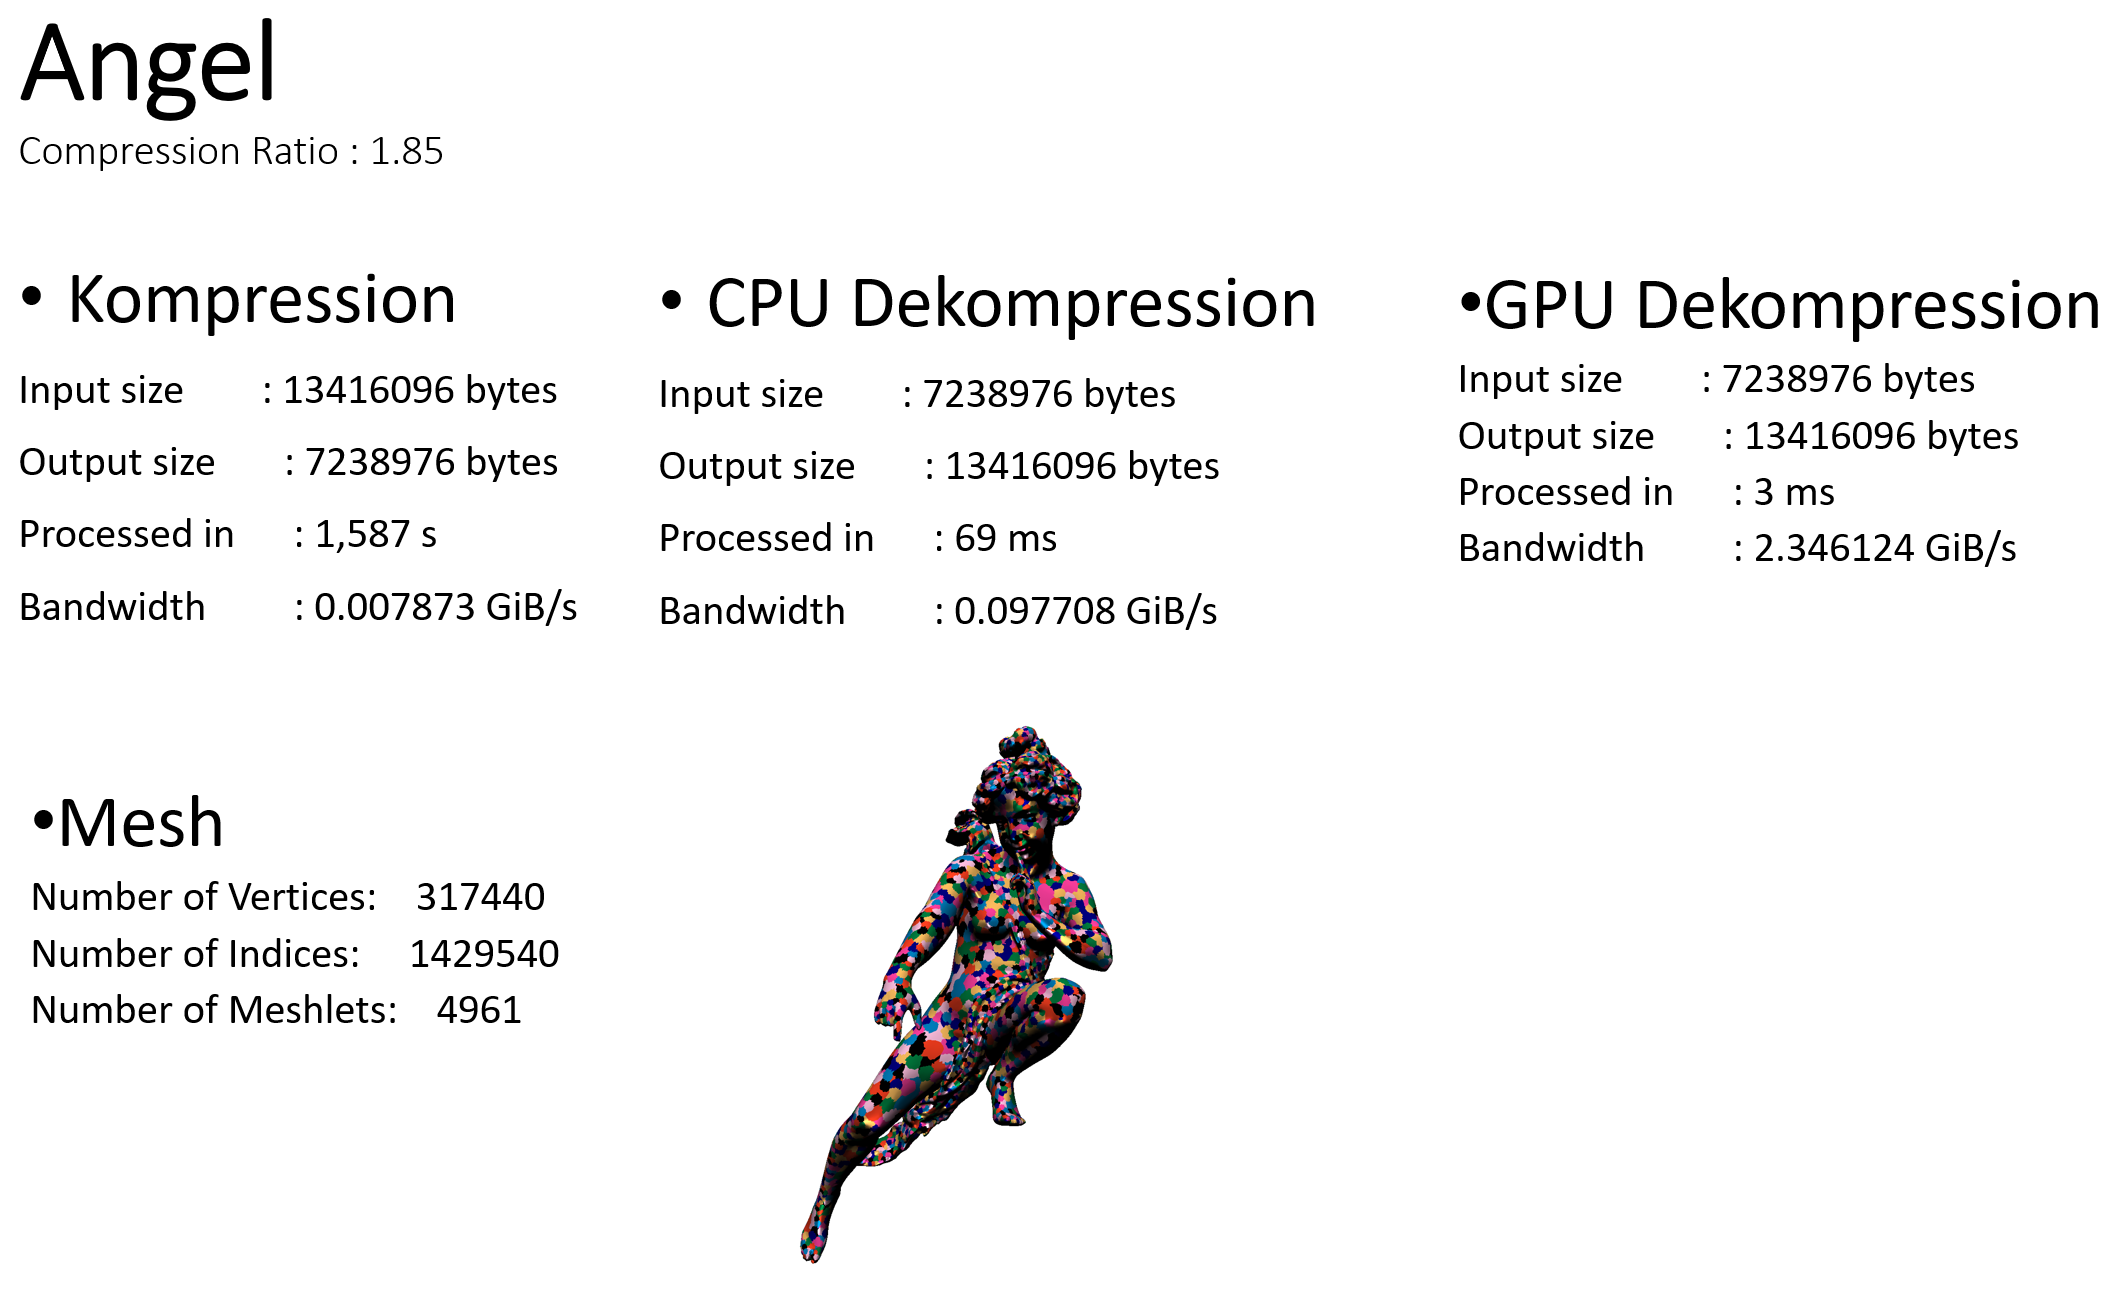
\includegraphics[scale=0.28]{Bilder/ergebnisse_full/angel.png}
\end{figure}
\begin{figure}[h]
  \centering  
  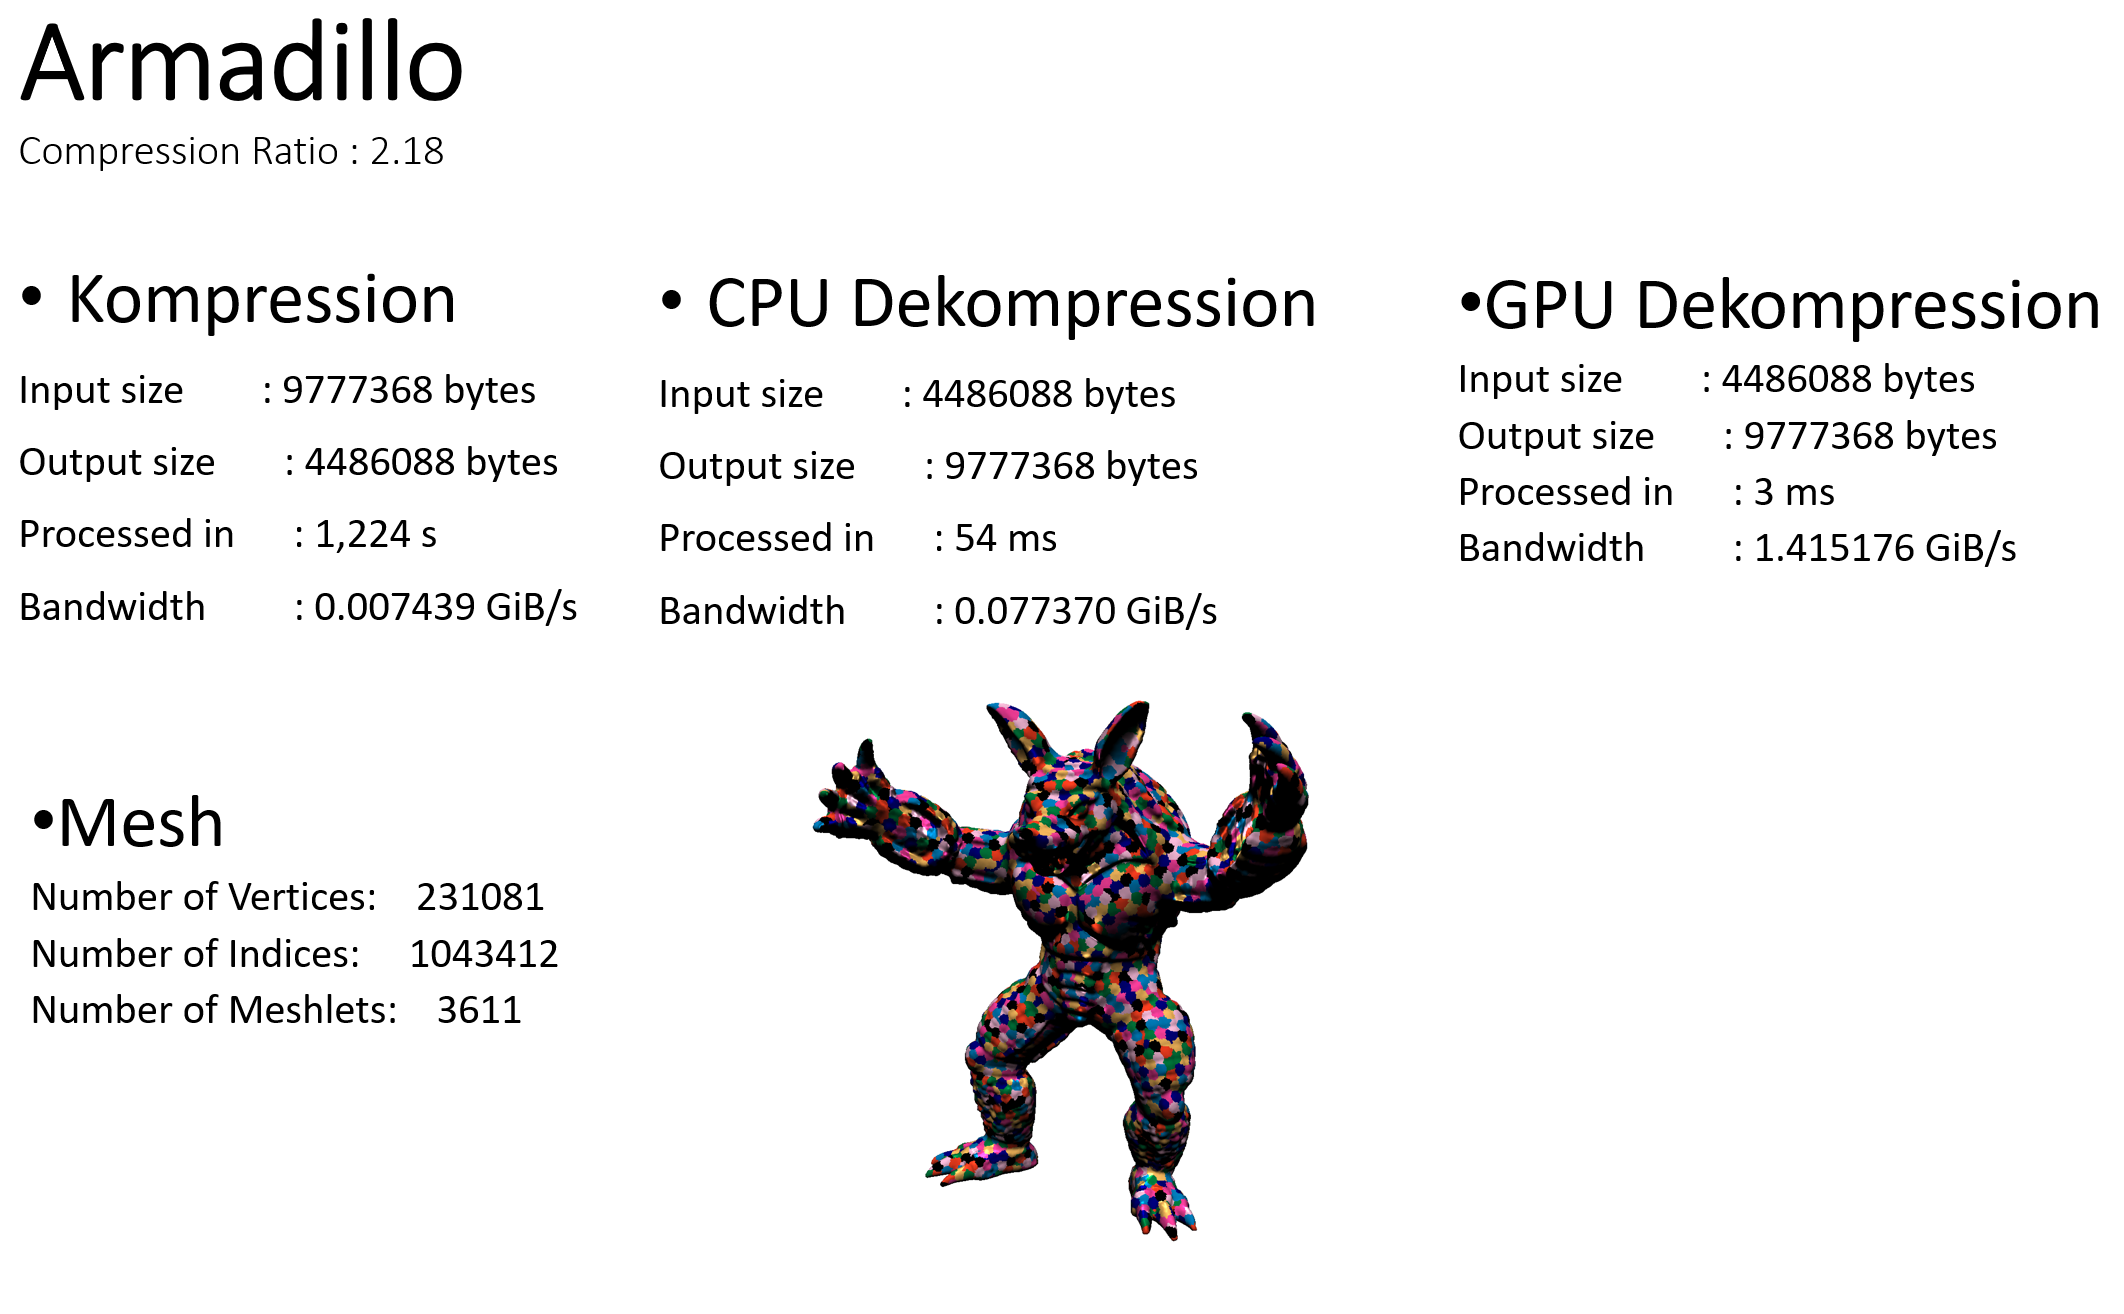
\includegraphics[scale=0.28]{Bilder/ergebnisse_full/armadillo.png}
\end{figure}
\begin{figure}[h]
  \centering  
  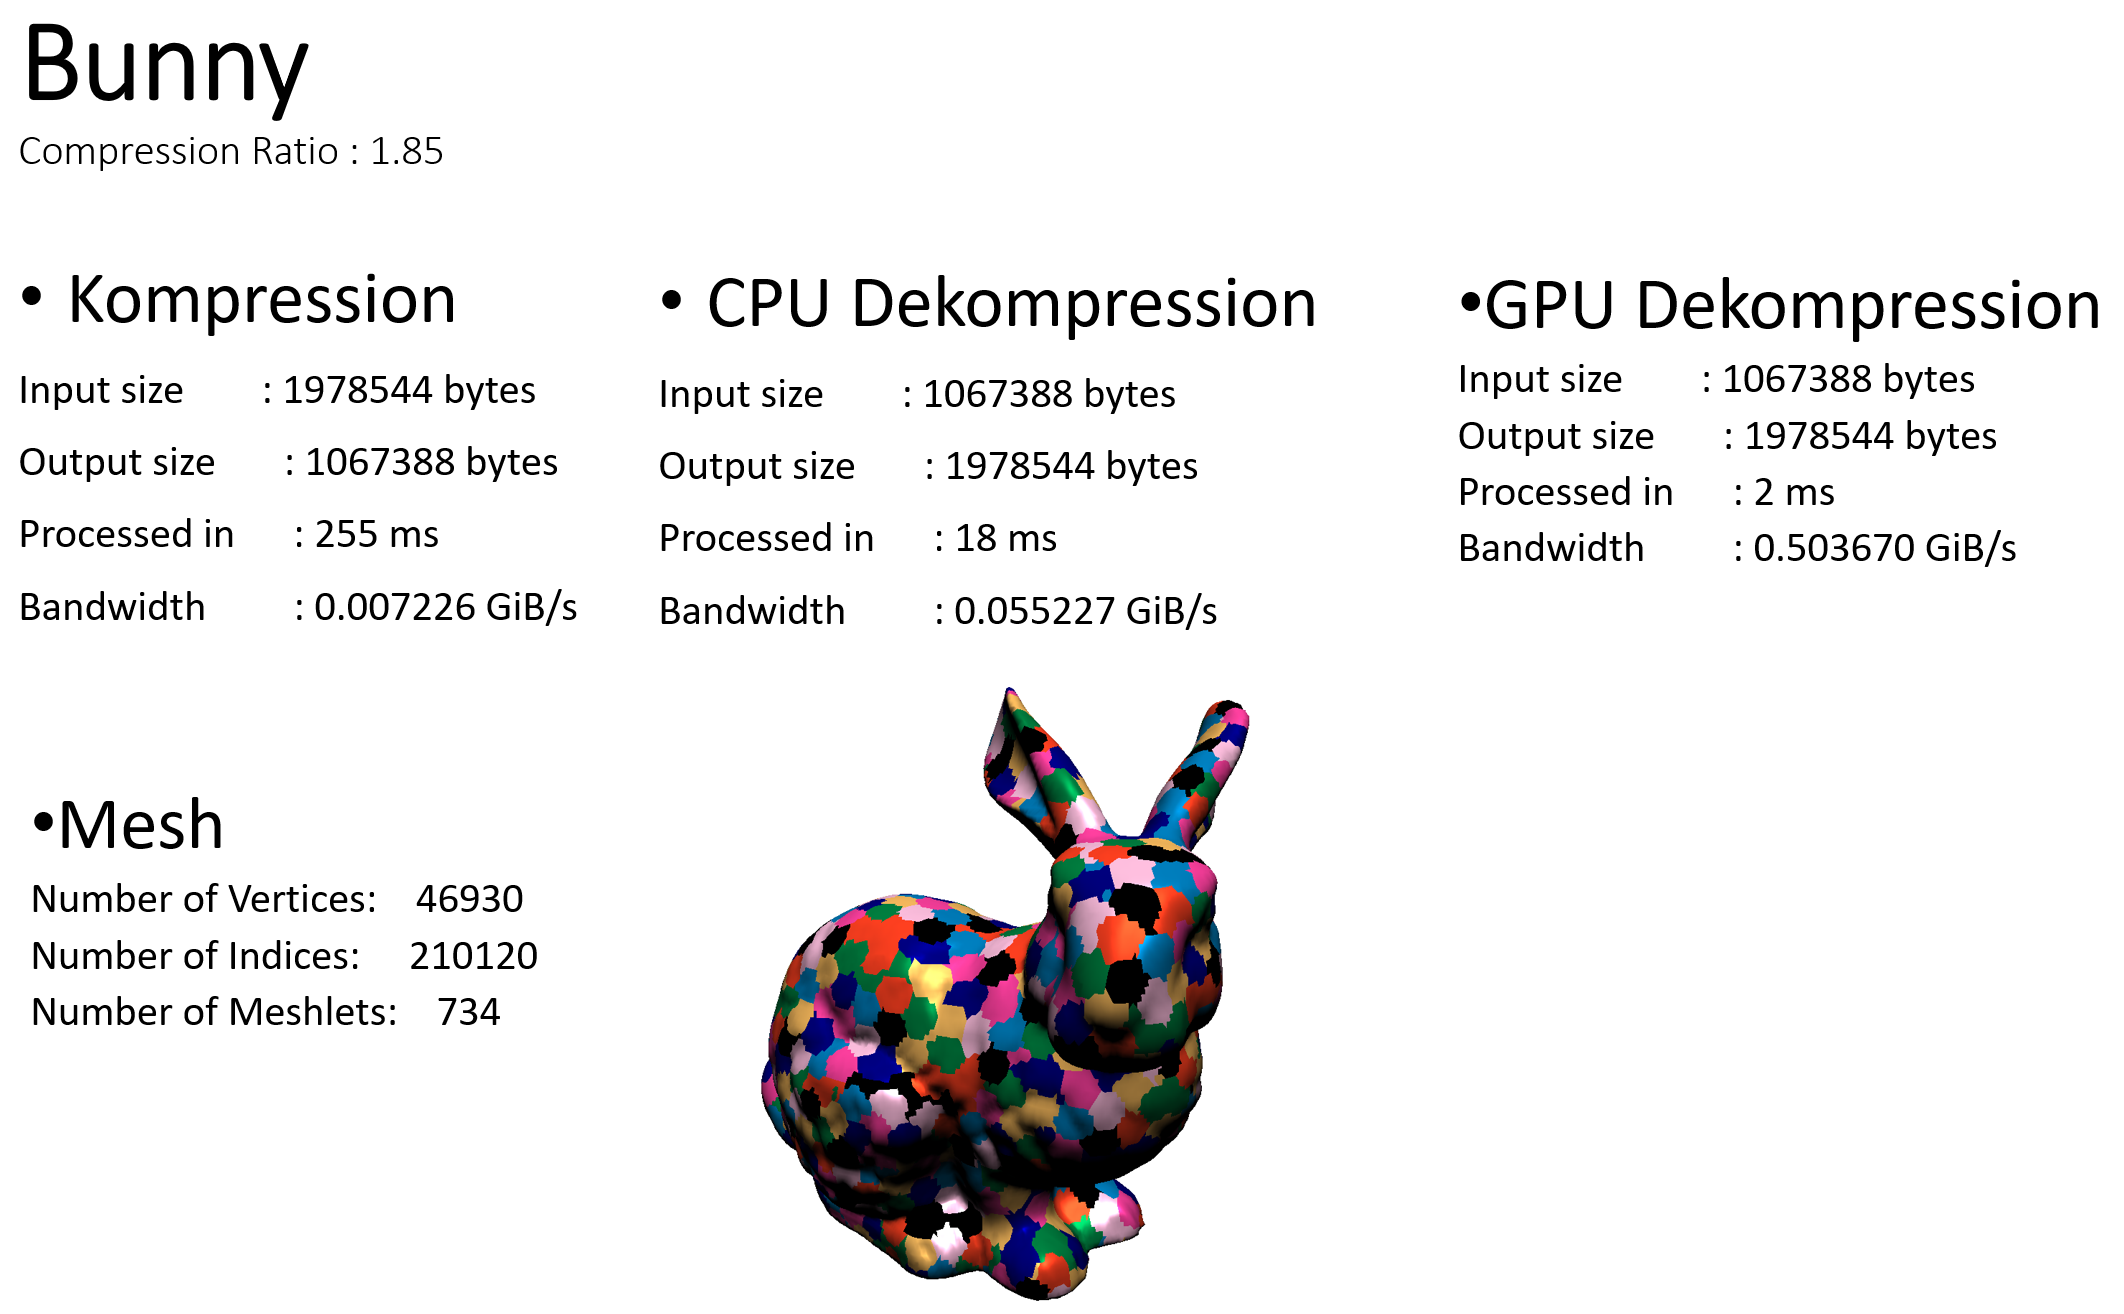
\includegraphics[scale=0.28]{Bilder/ergebnisse_full/bunny.png}
\end{figure}
\begin{figure}[h]
  \centering  
  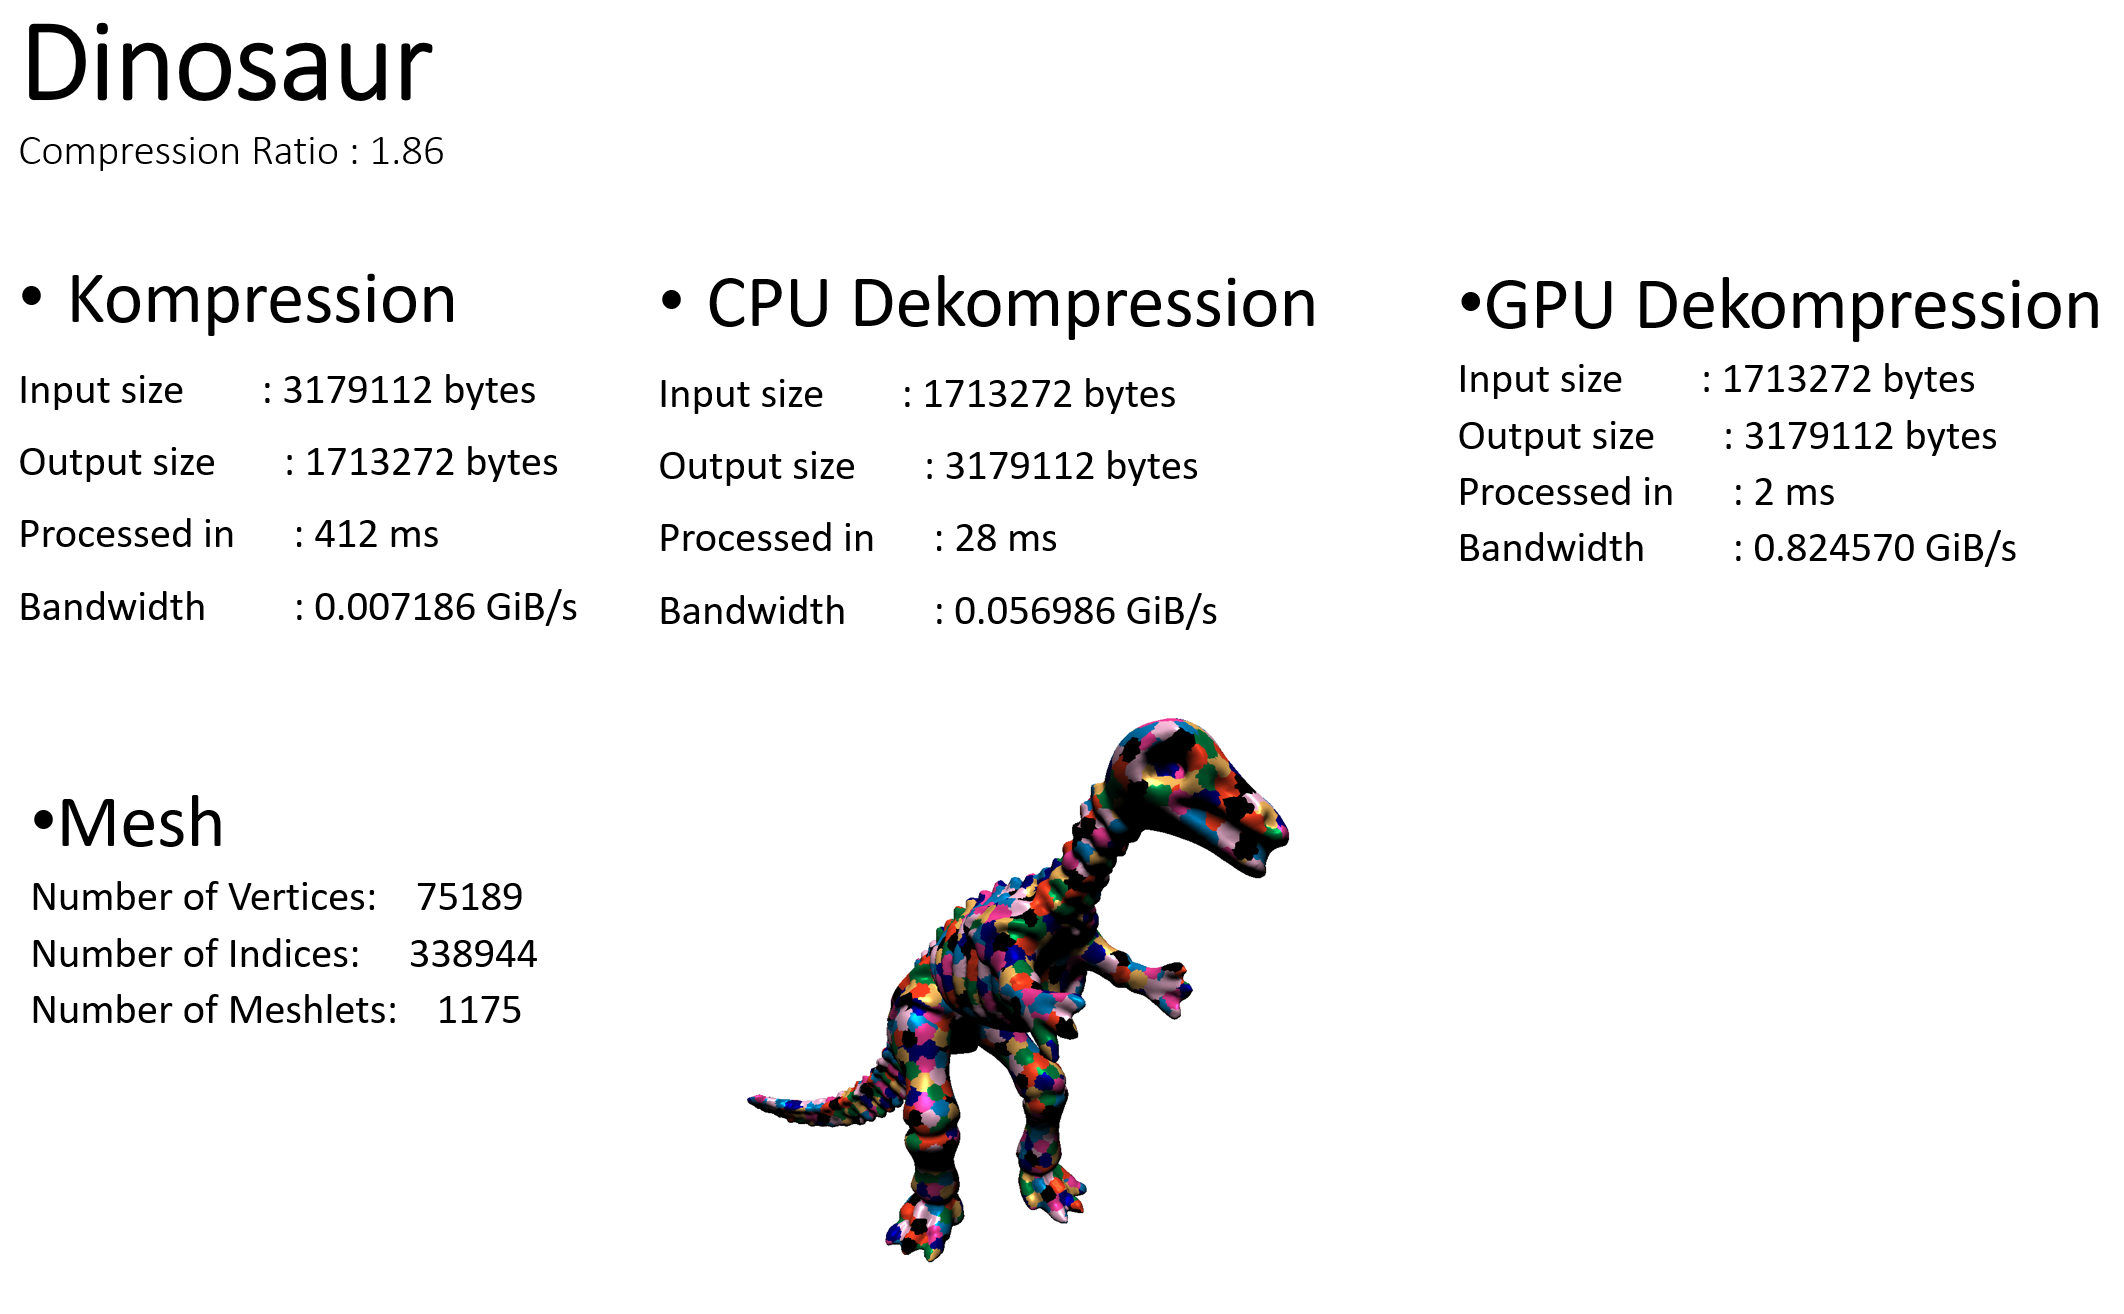
\includegraphics[scale=0.28]{Bilder/ergebnisse_full/dinosaur.png}
\end{figure}
\begin{figure}[h]
  \centering  
  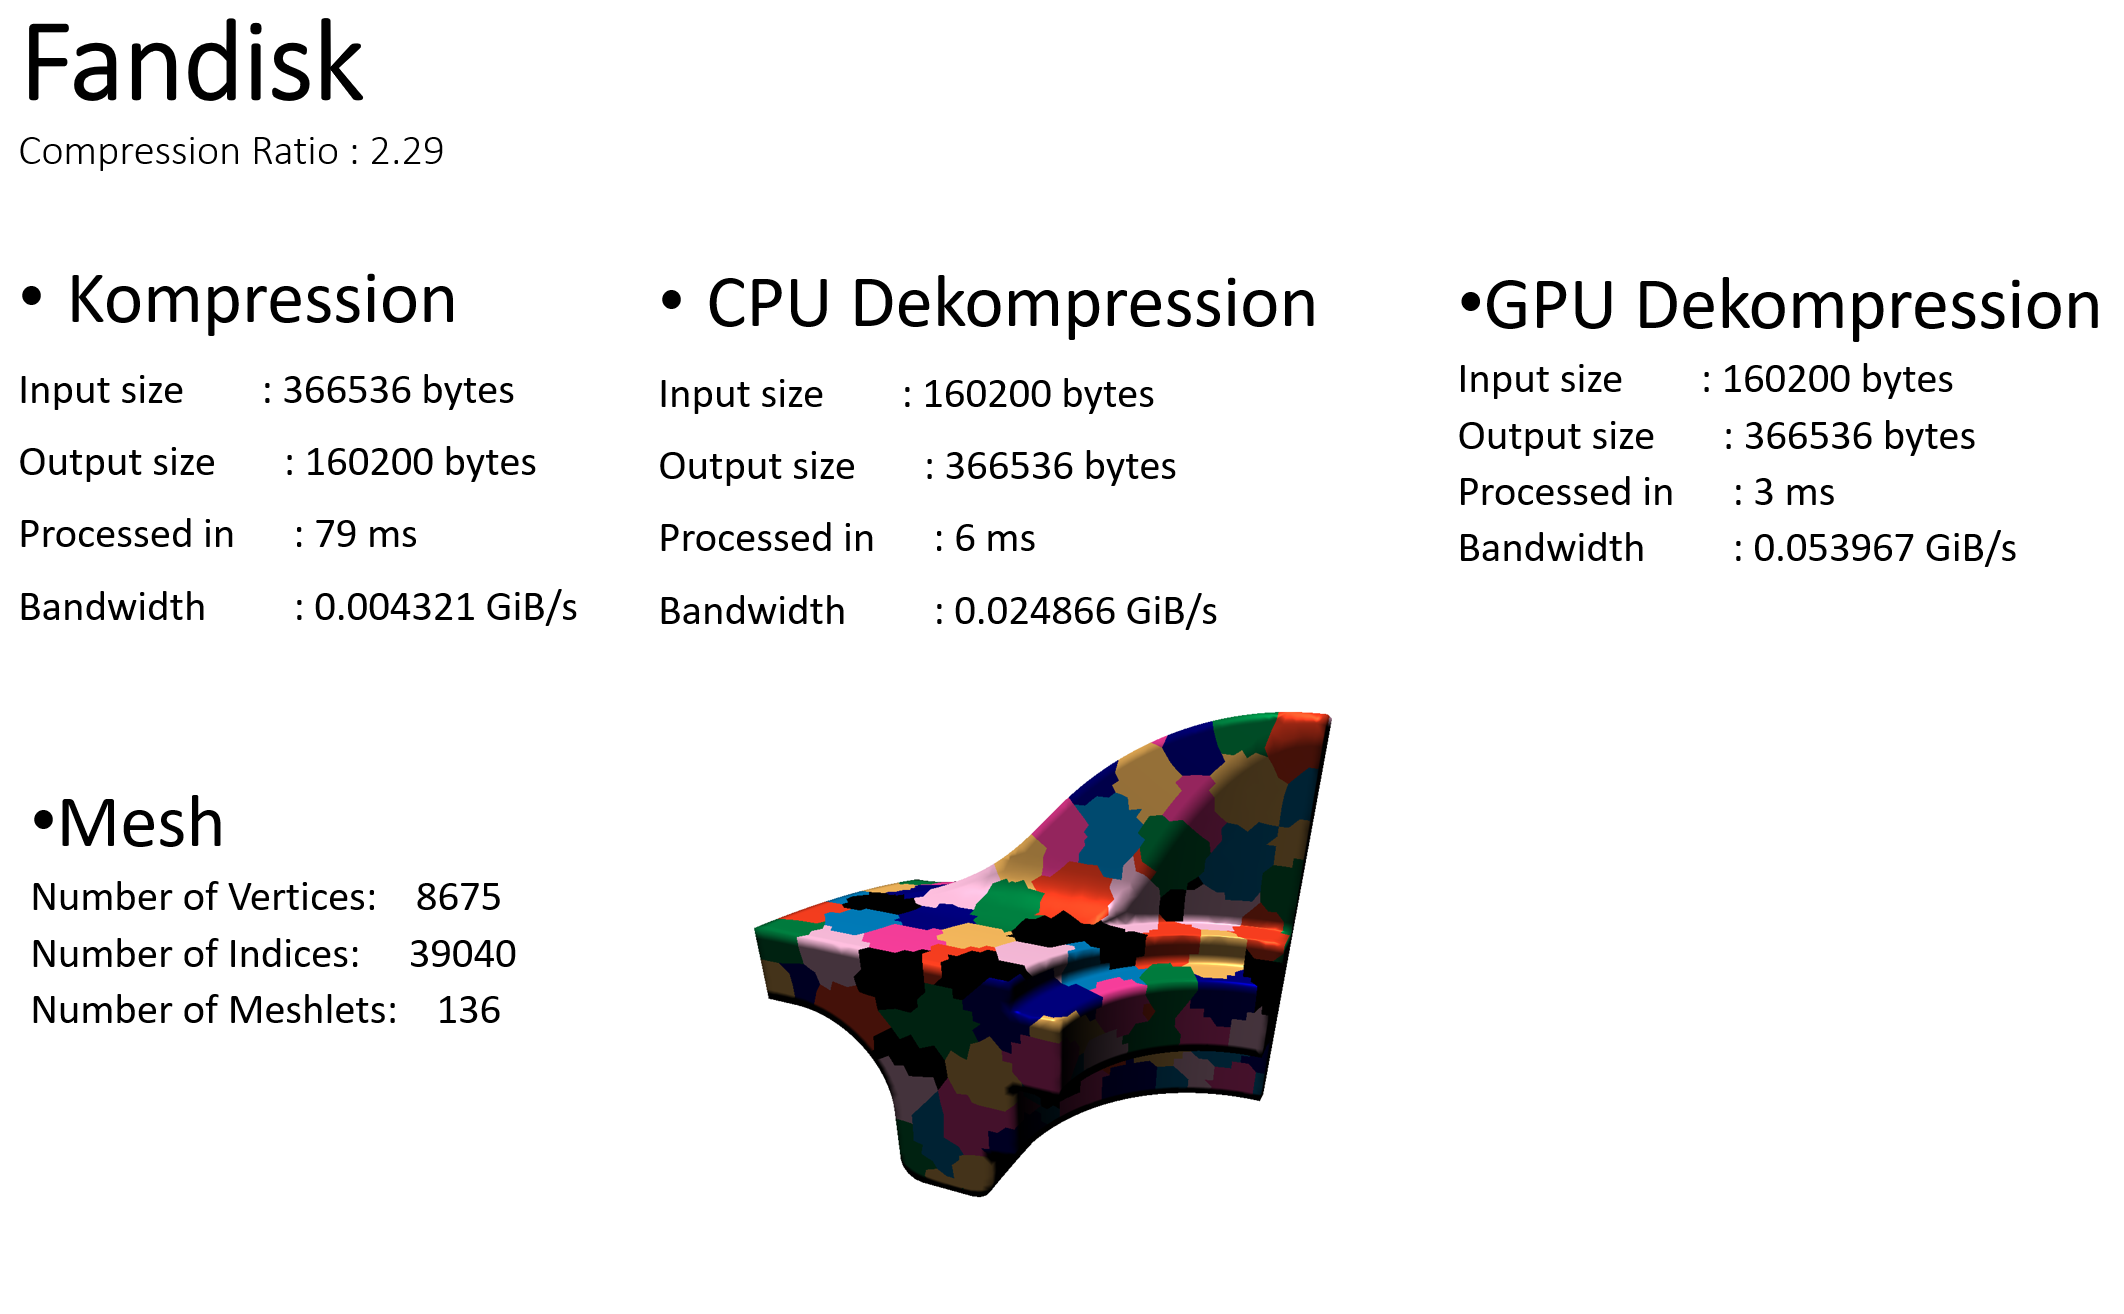
\includegraphics[scale=0.28]{Bilder/ergebnisse_full/fandisk.png}
\end{figure}
\begin{figure}[h]
  \centering  
  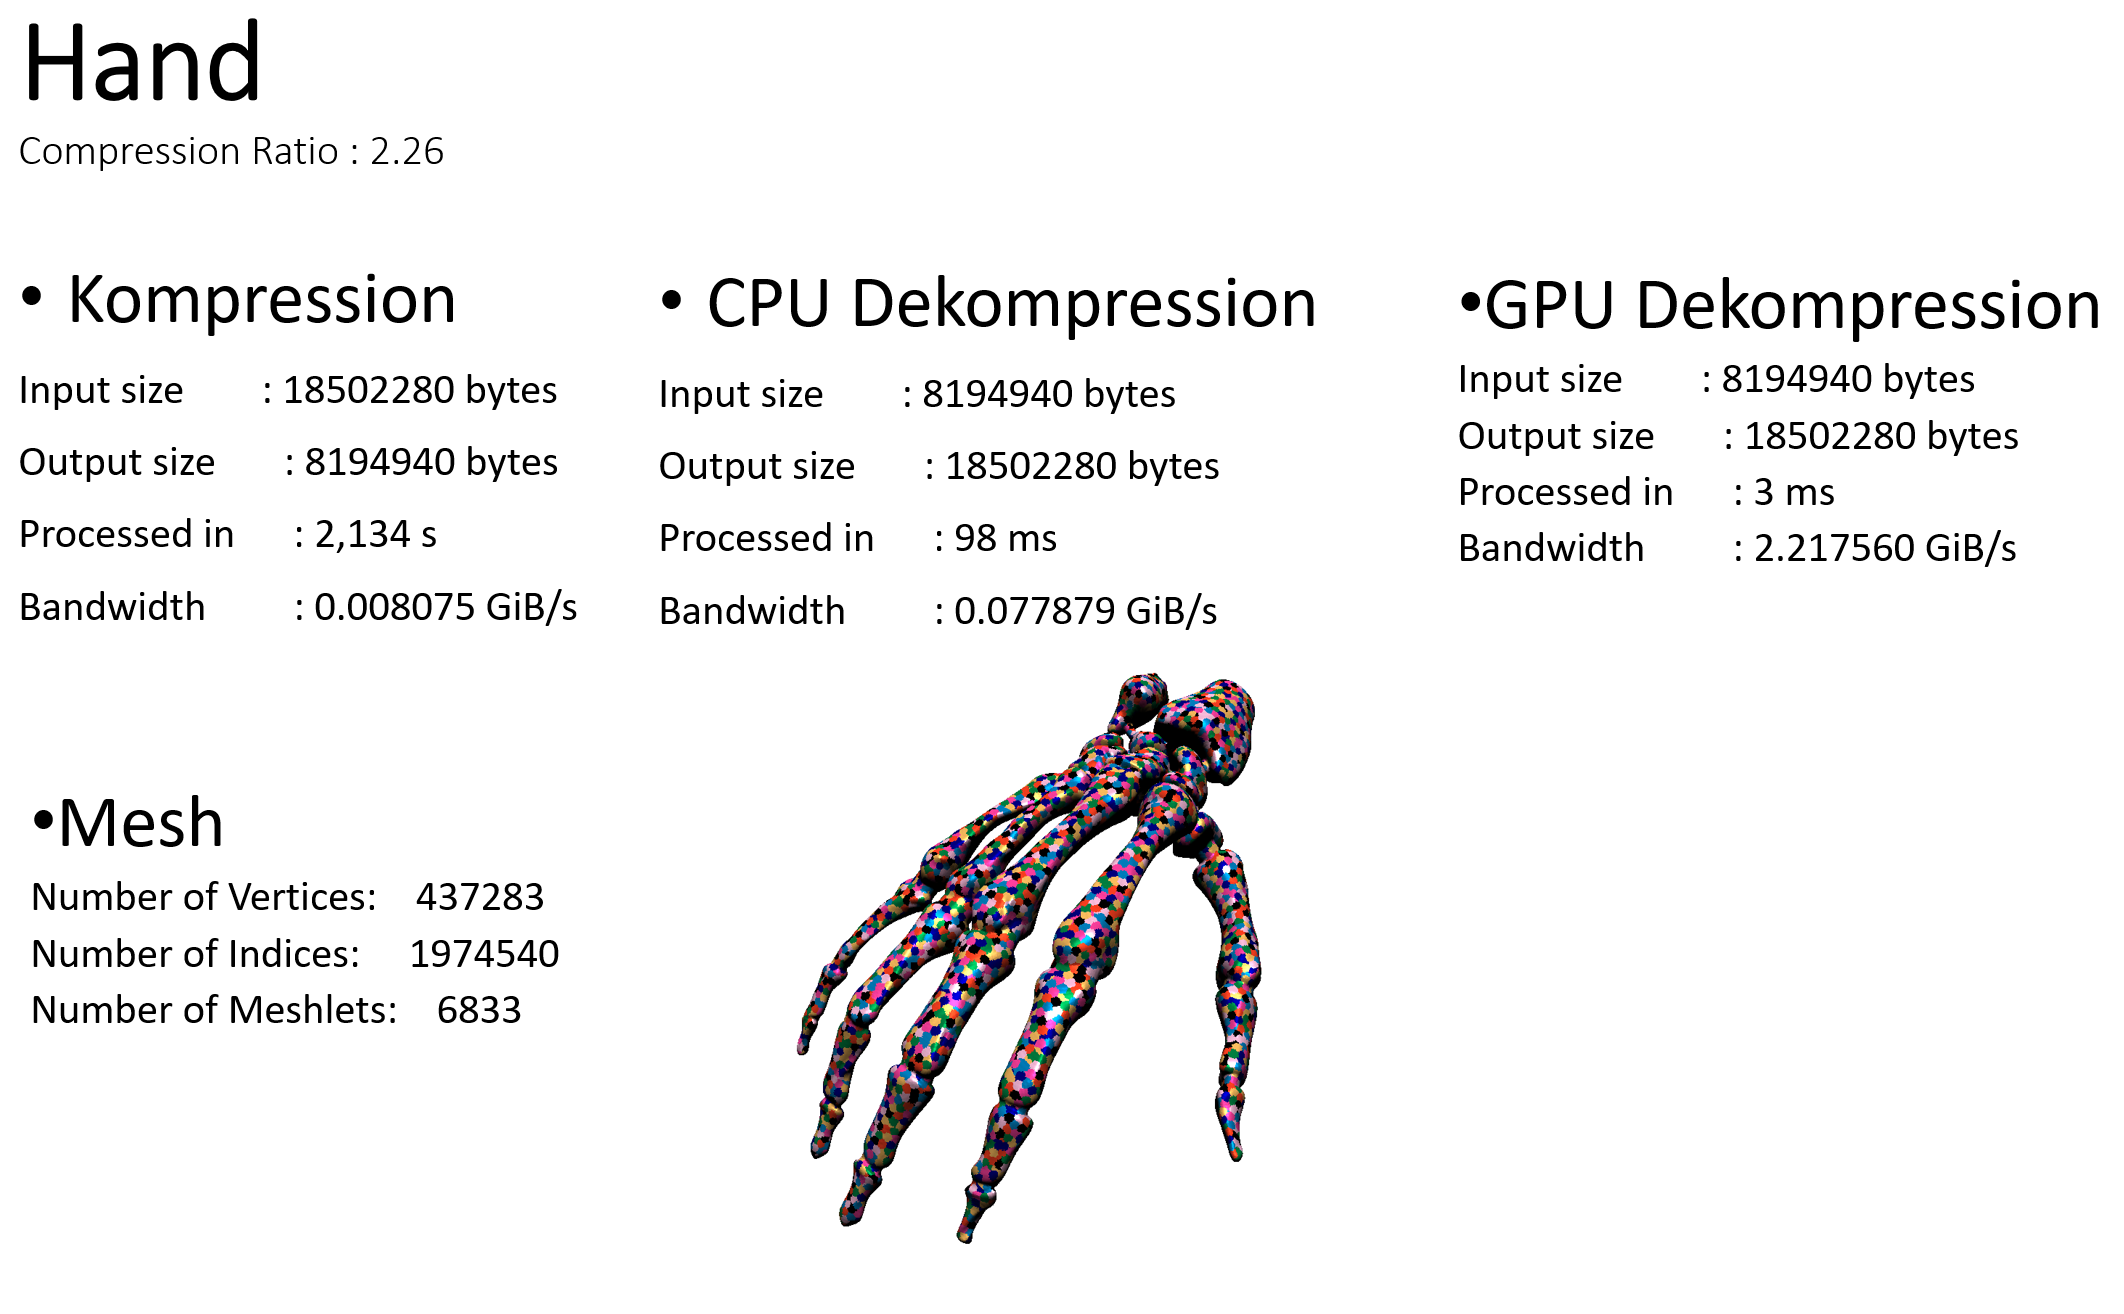
\includegraphics[scale=0.28]{Bilder/ergebnisse_full/hand.png}
\end{figure}
\begin{figure}[h]
  \centering  
  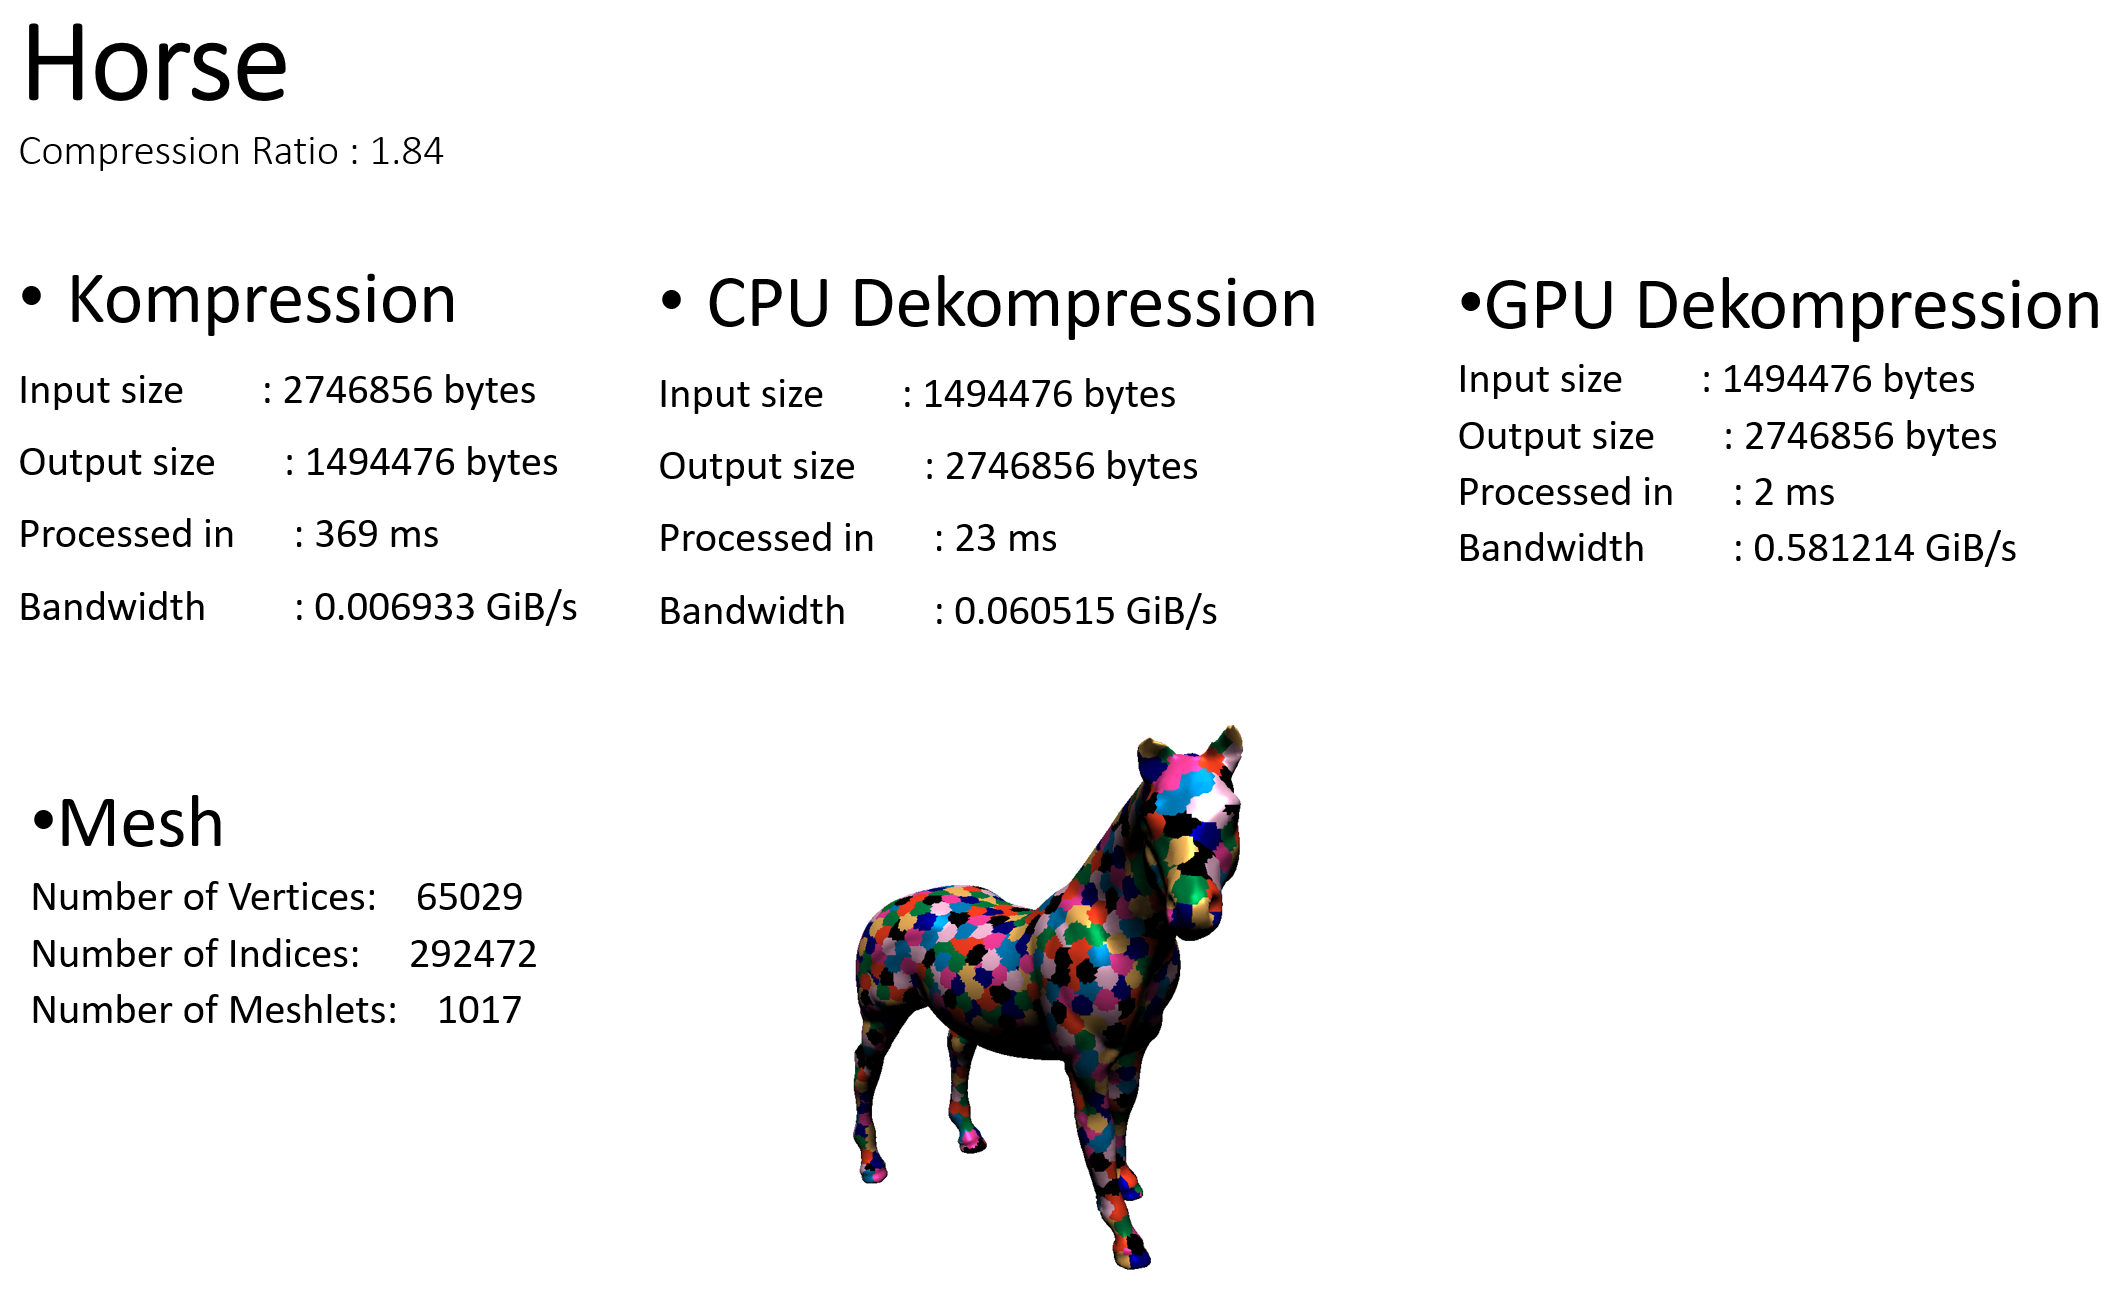
\includegraphics[scale=0.28]{Bilder/ergebnisse_full/horse.png}
\end{figure}
\begin{figure}[h]
  \centering  
  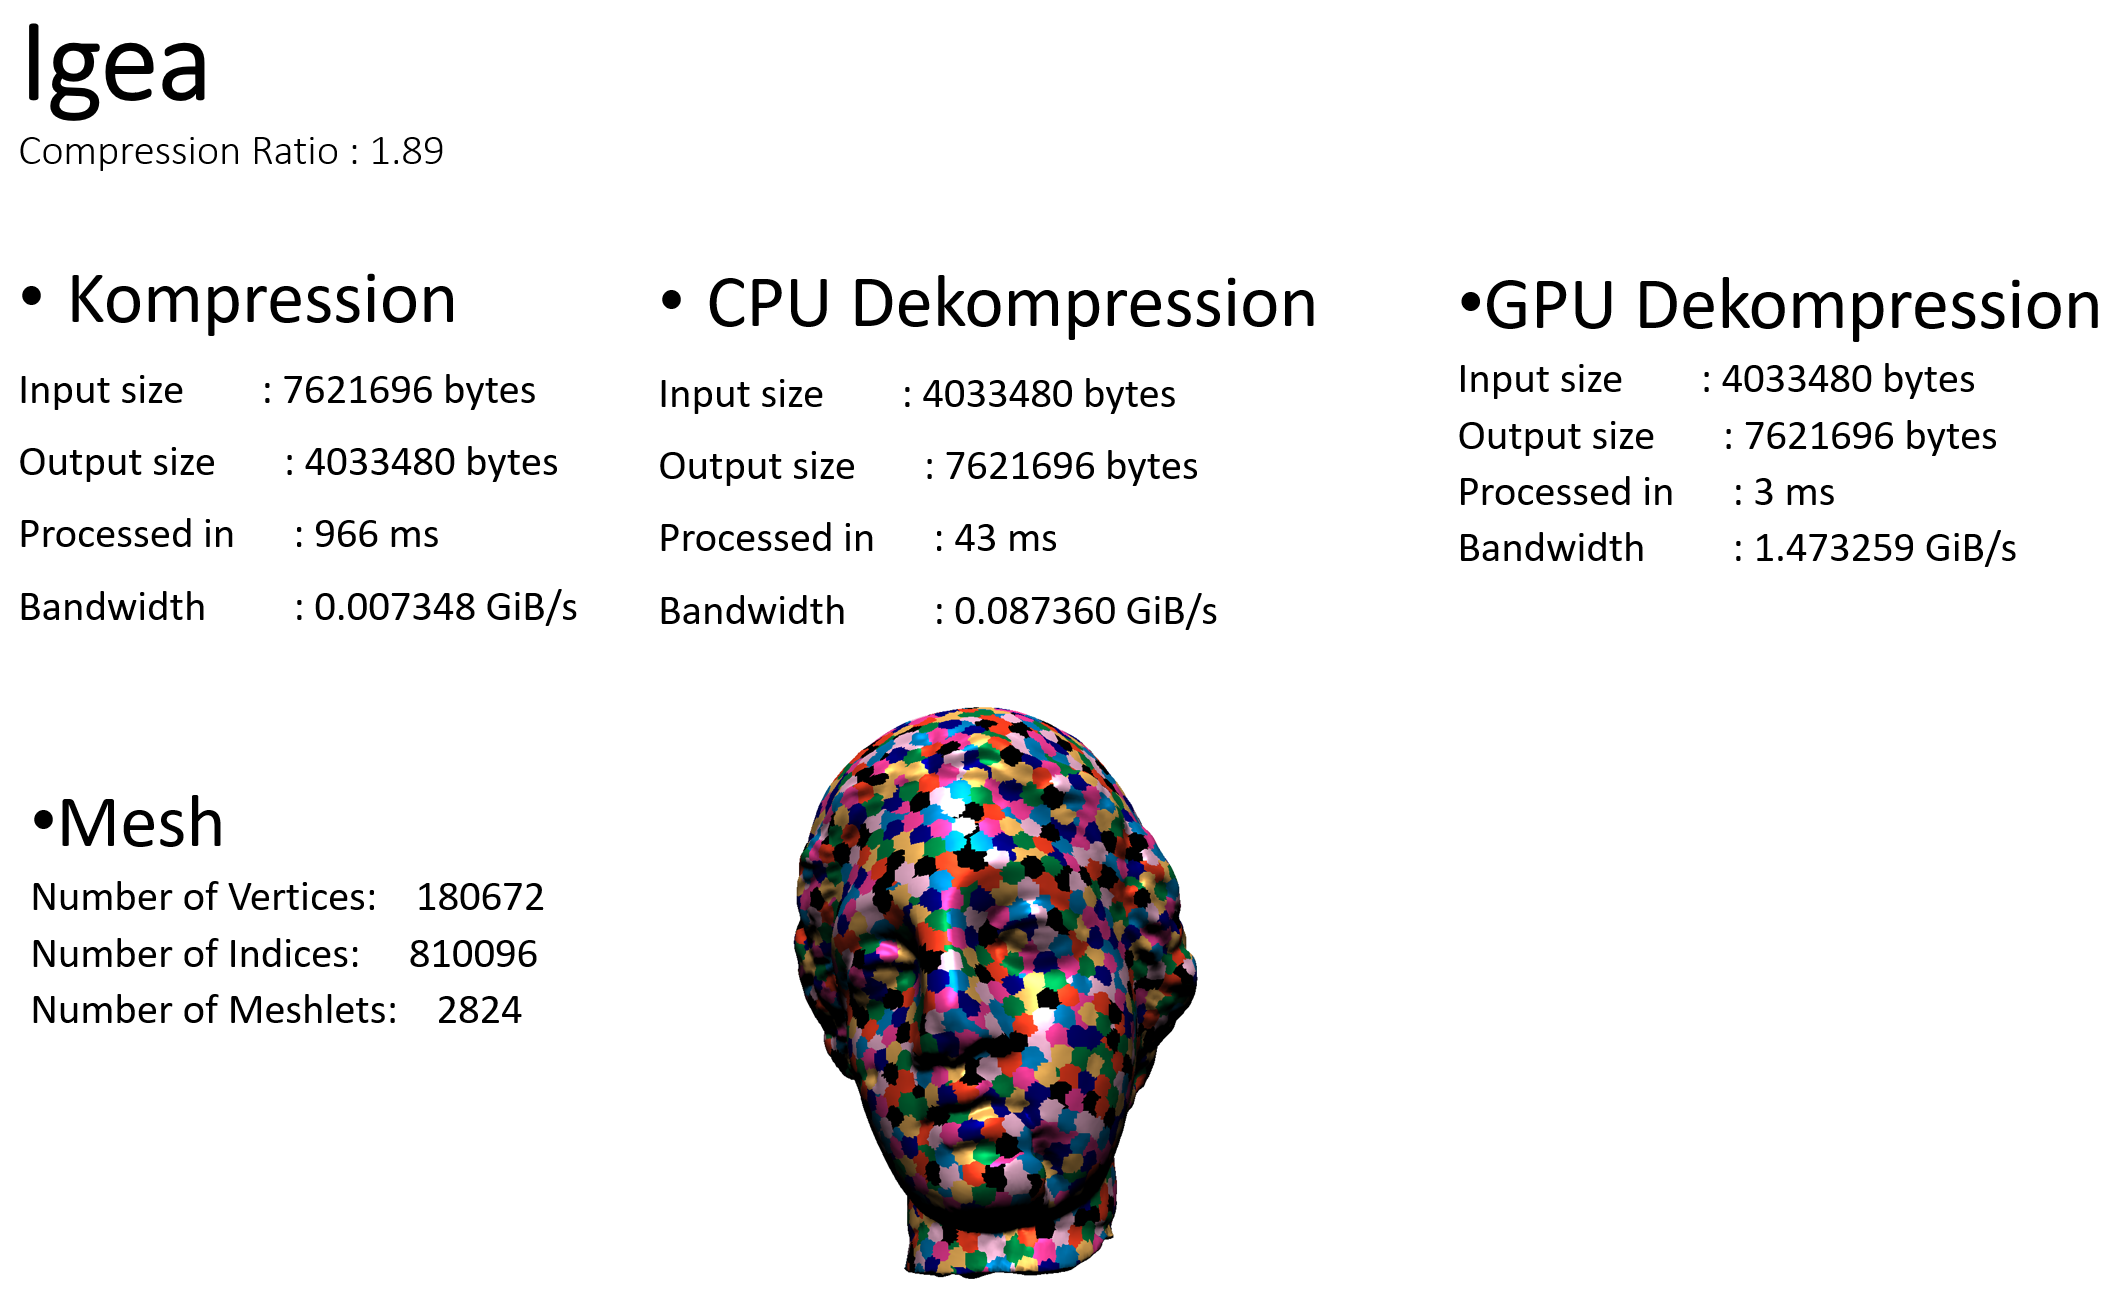
\includegraphics[scale=0.28]{Bilder/ergebnisse_full/igea.png}
\end{figure}
\begin{figure}[h]
  \centering  
  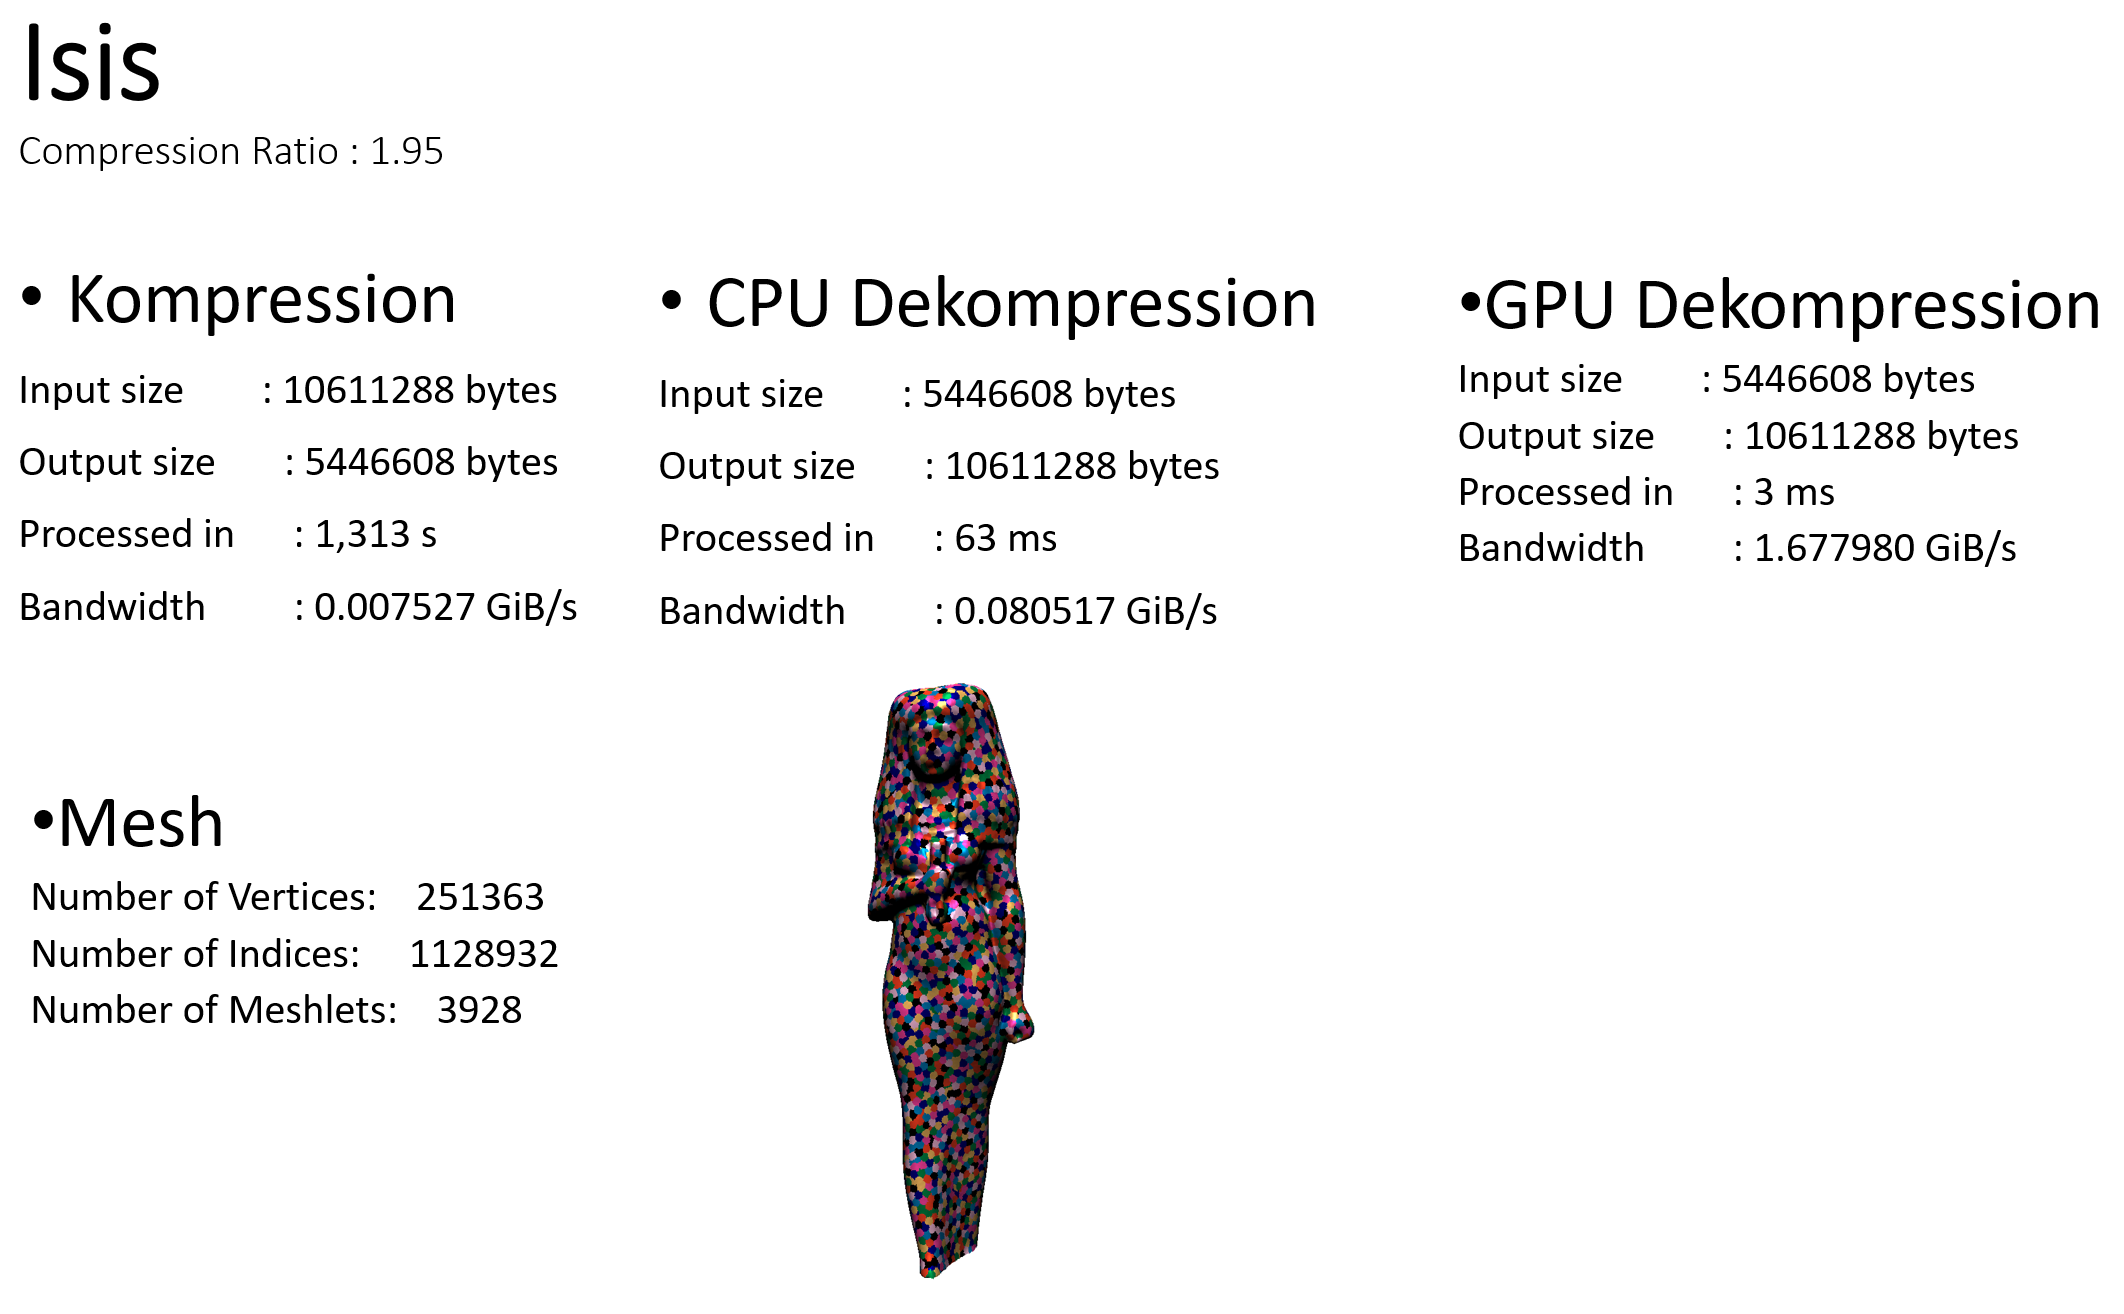
\includegraphics[scale=0.28]{Bilder/ergebnisse_full/isis.png}
\end{figure}
\begin{figure}[h]
  \centering  
  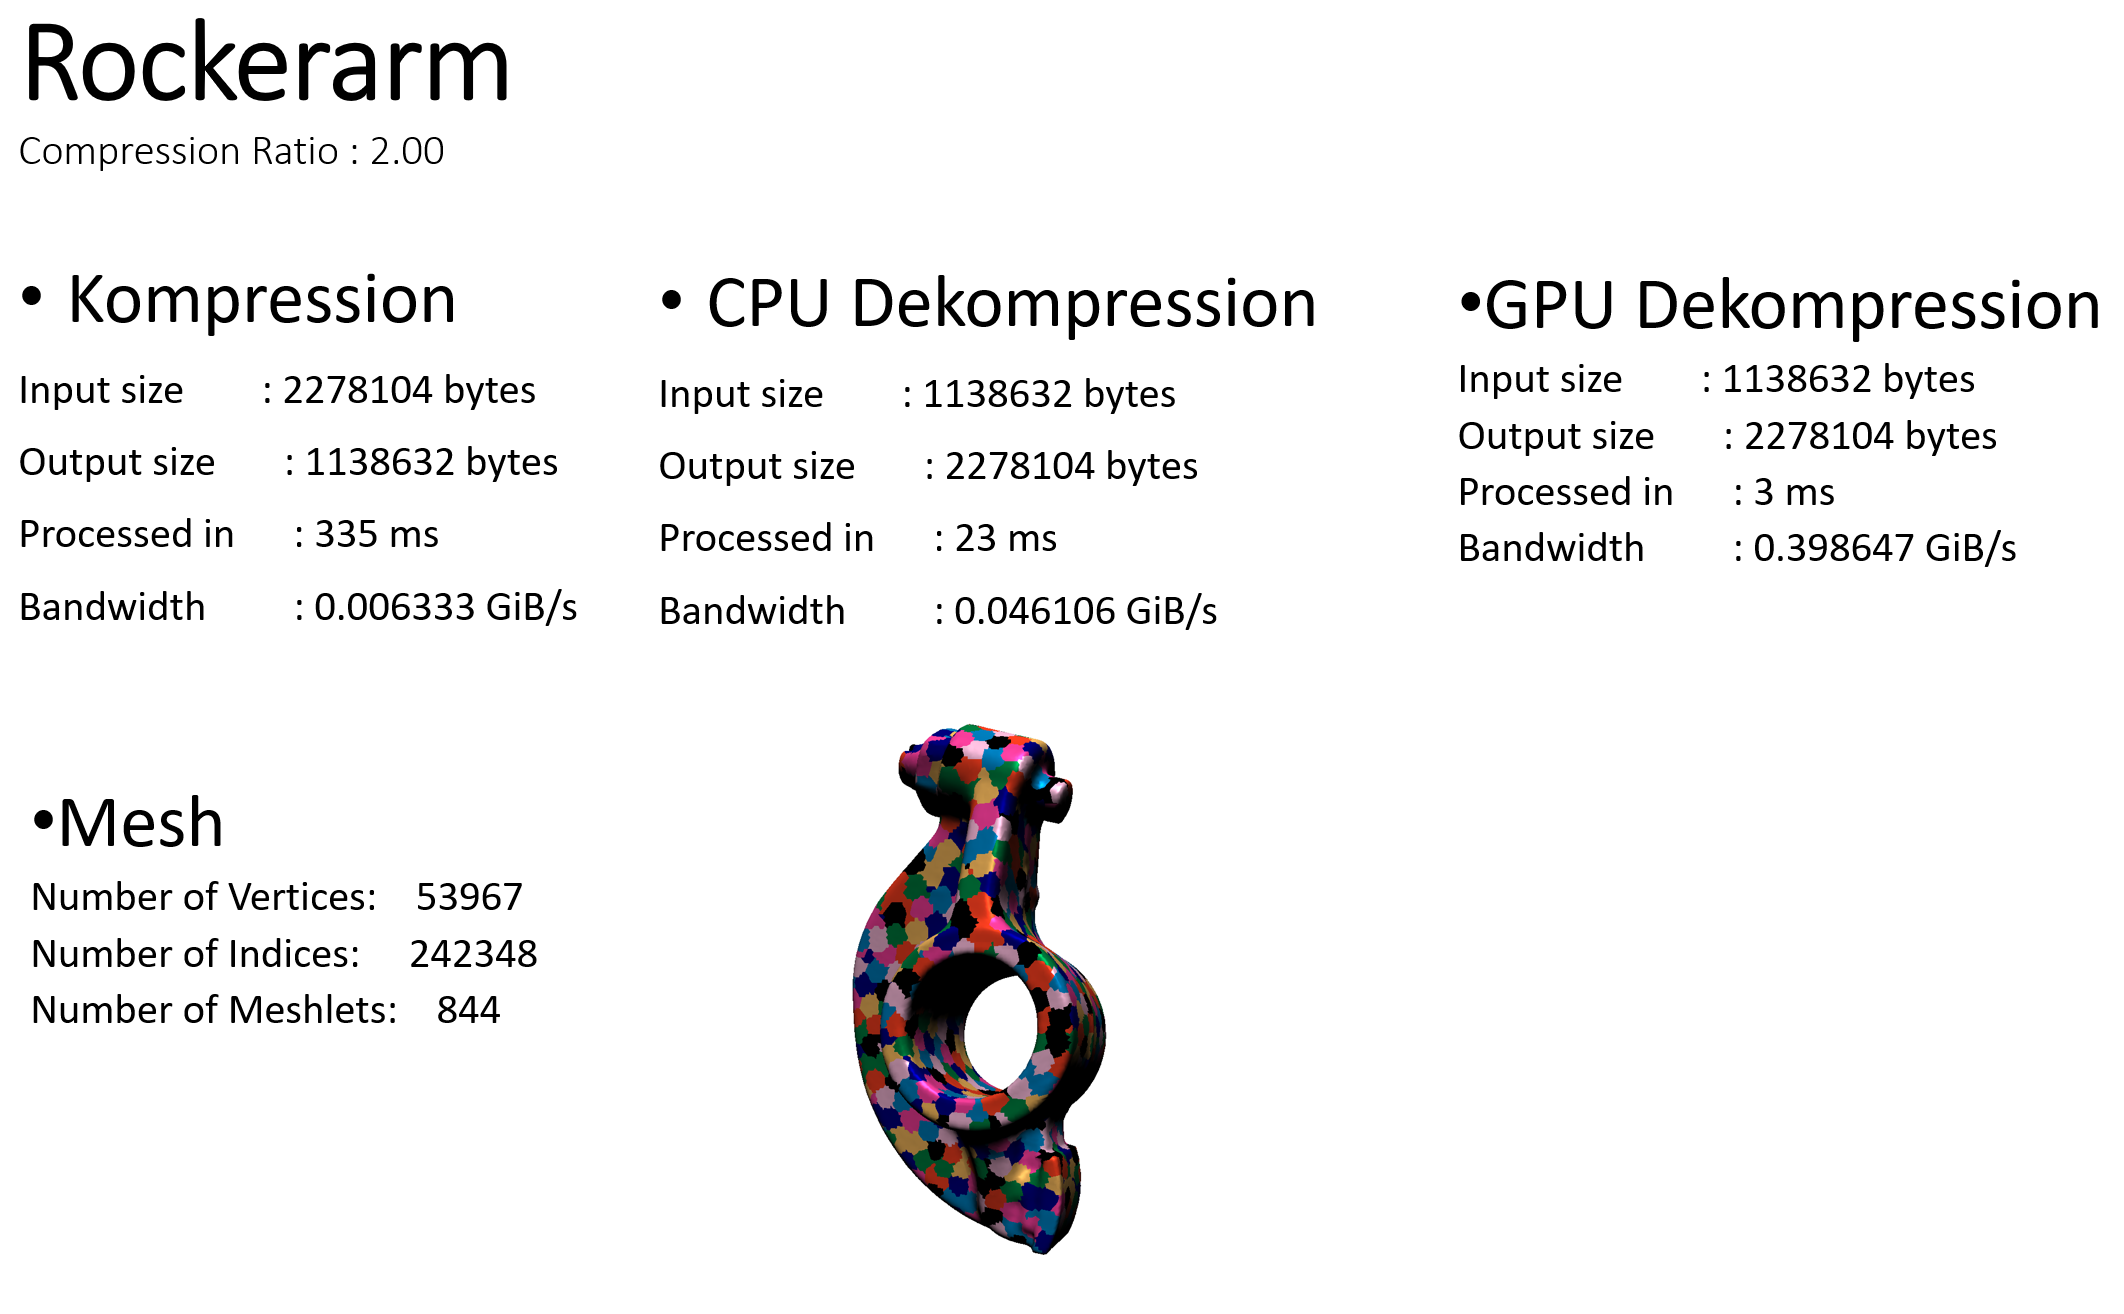
\includegraphics[scale=0.28]{Bilder/ergebnisse_full/rockerarm.png}
\end{figure}
\begin{figure}[h]
  \centering  
  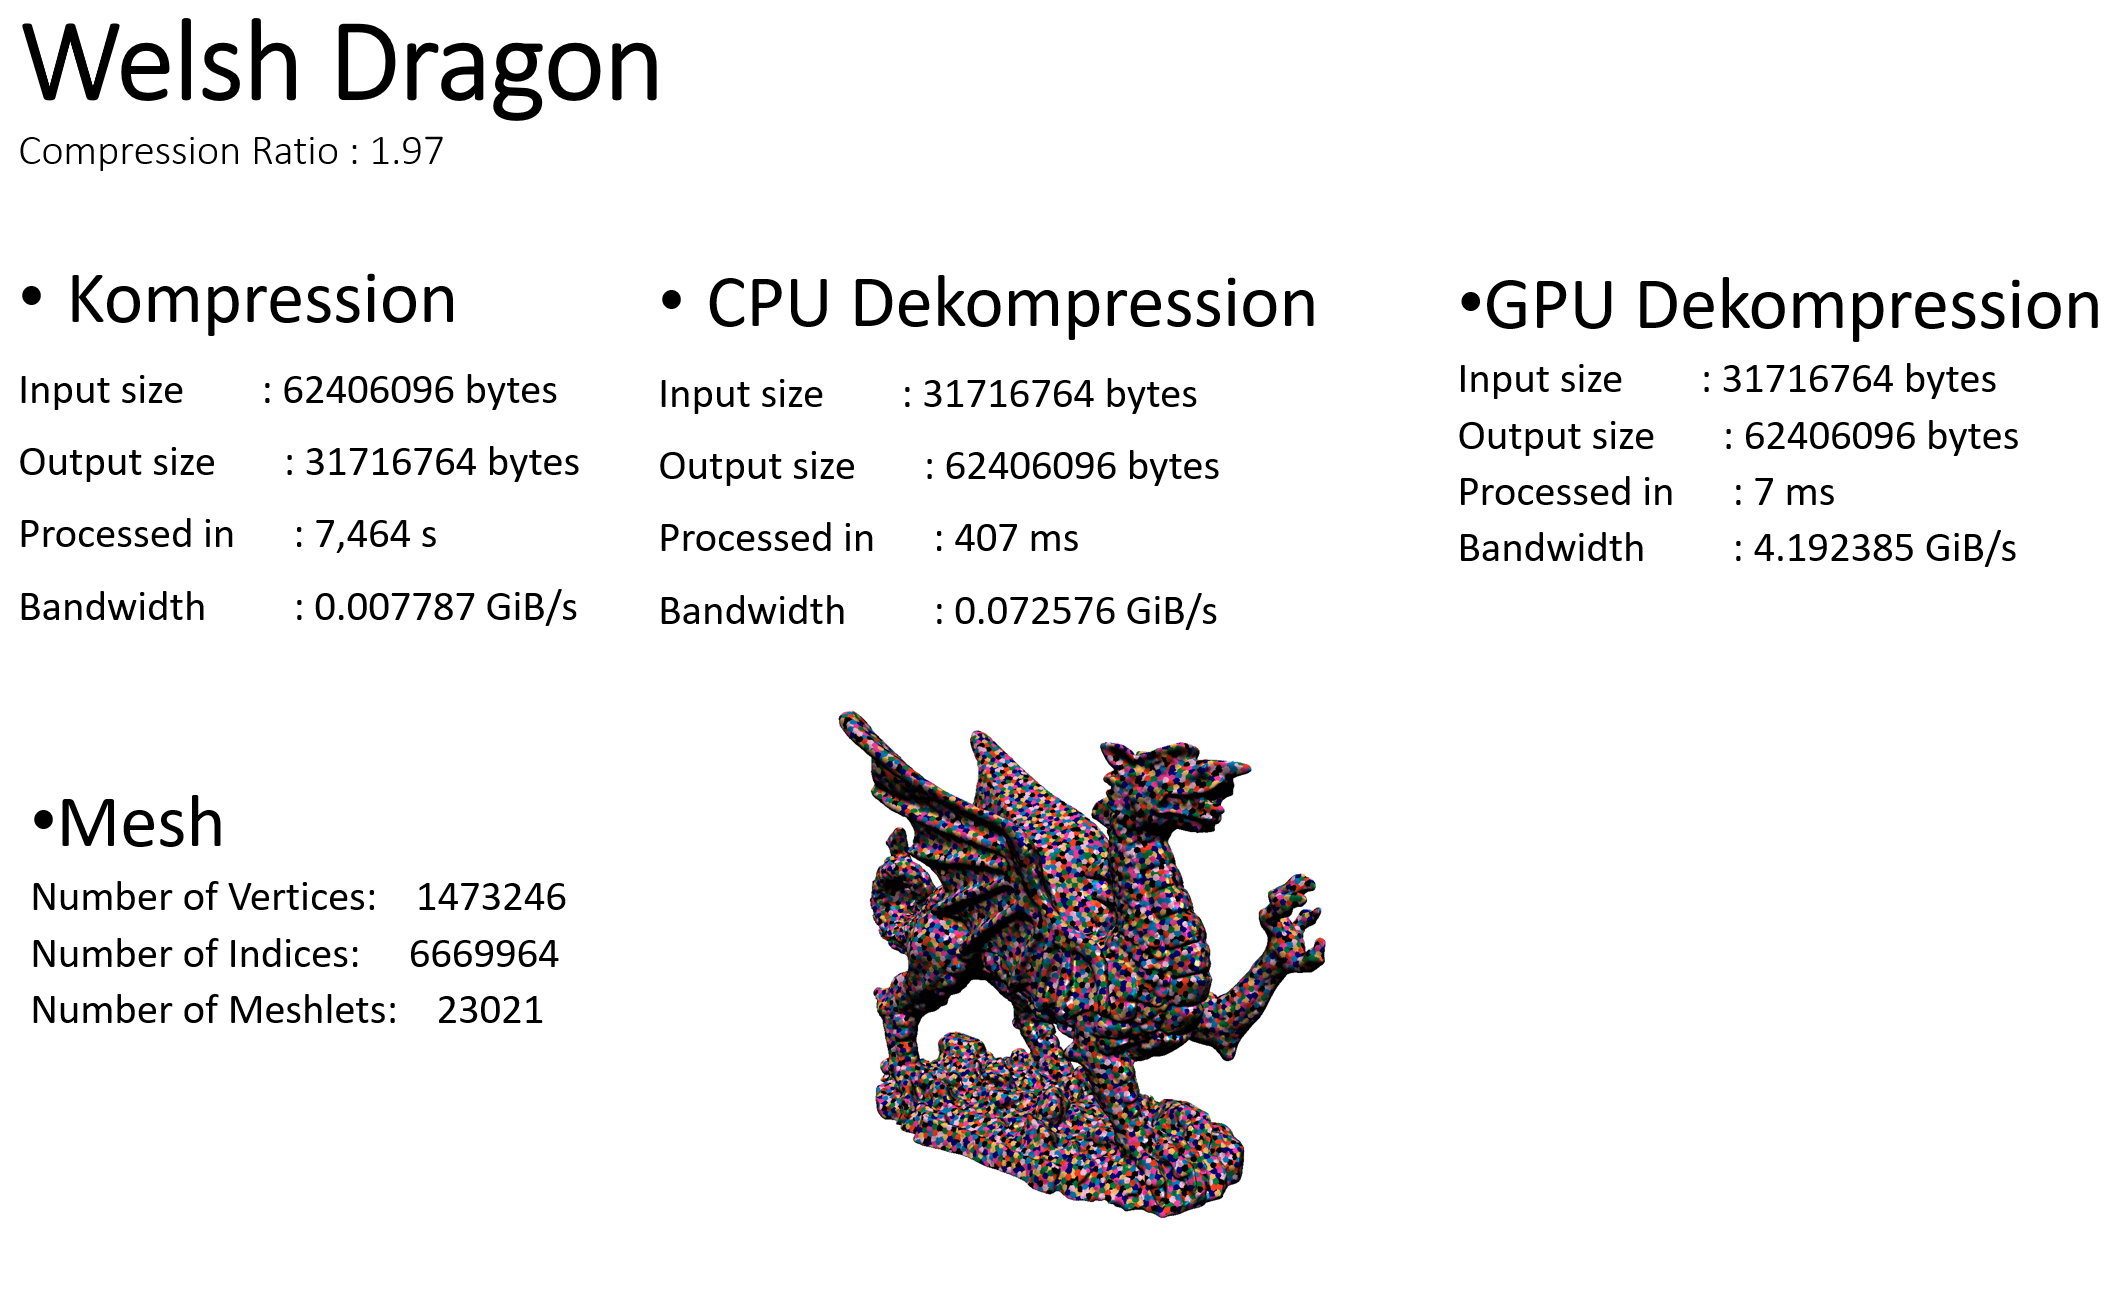
\includegraphics[scale=0.28]{Bilder/ergebnisse_full/welshdragon.png}
\end{figure}
\begin{figure}[h]
  \centering  
  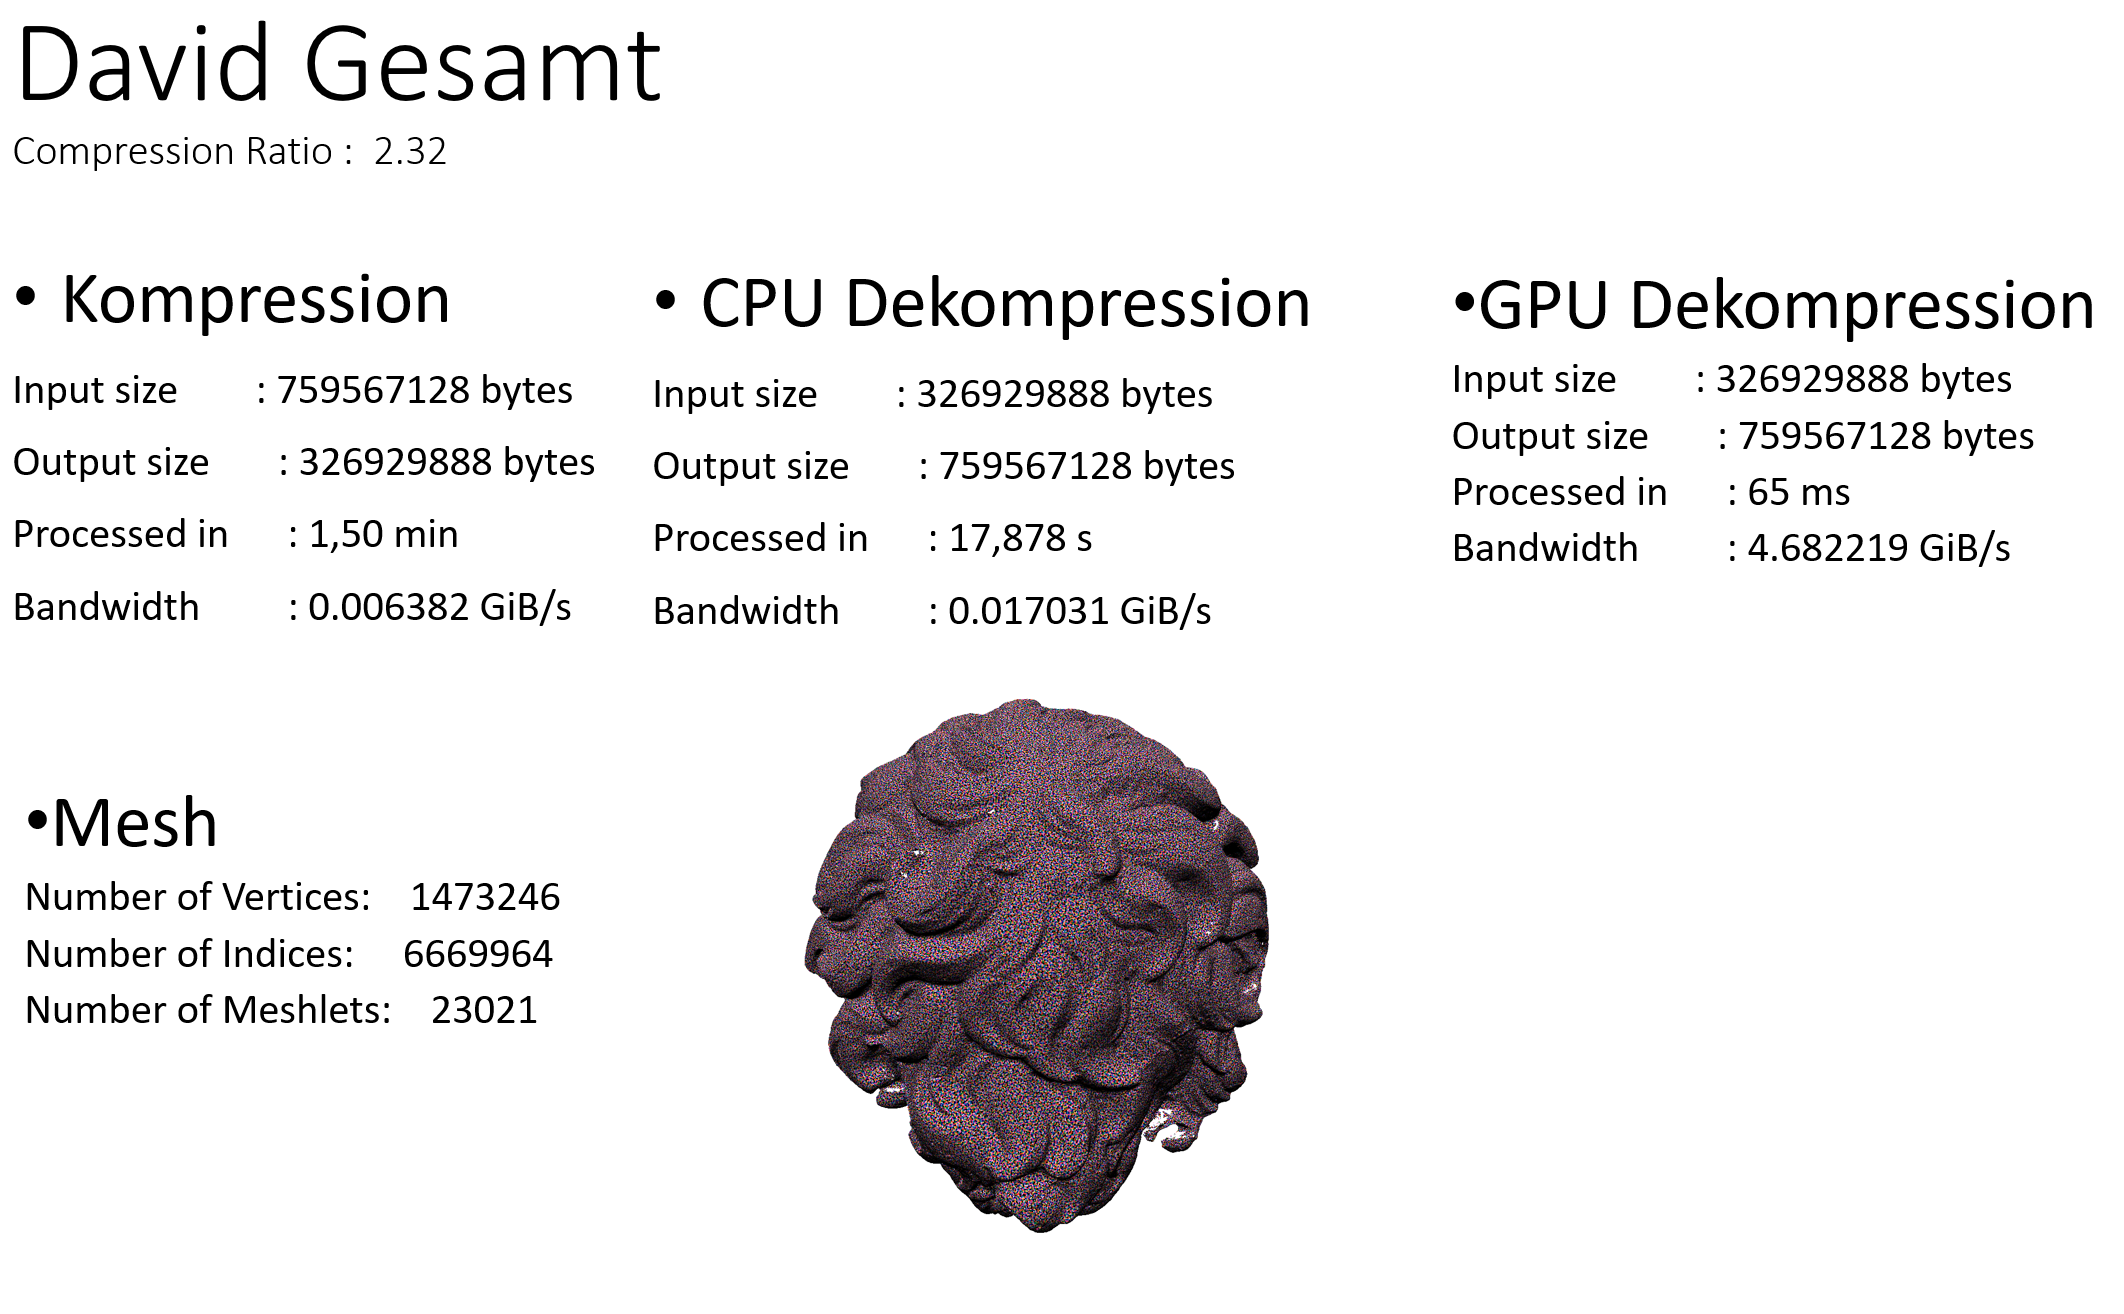
\includegraphics[scale=0.28]{Bilder/ergebnisse_full/david.png}
\end{figure}
\clearpage
\subsection{Ergebnisse mit Quantisierung}
\begin{figure}[h]
  \centering  
  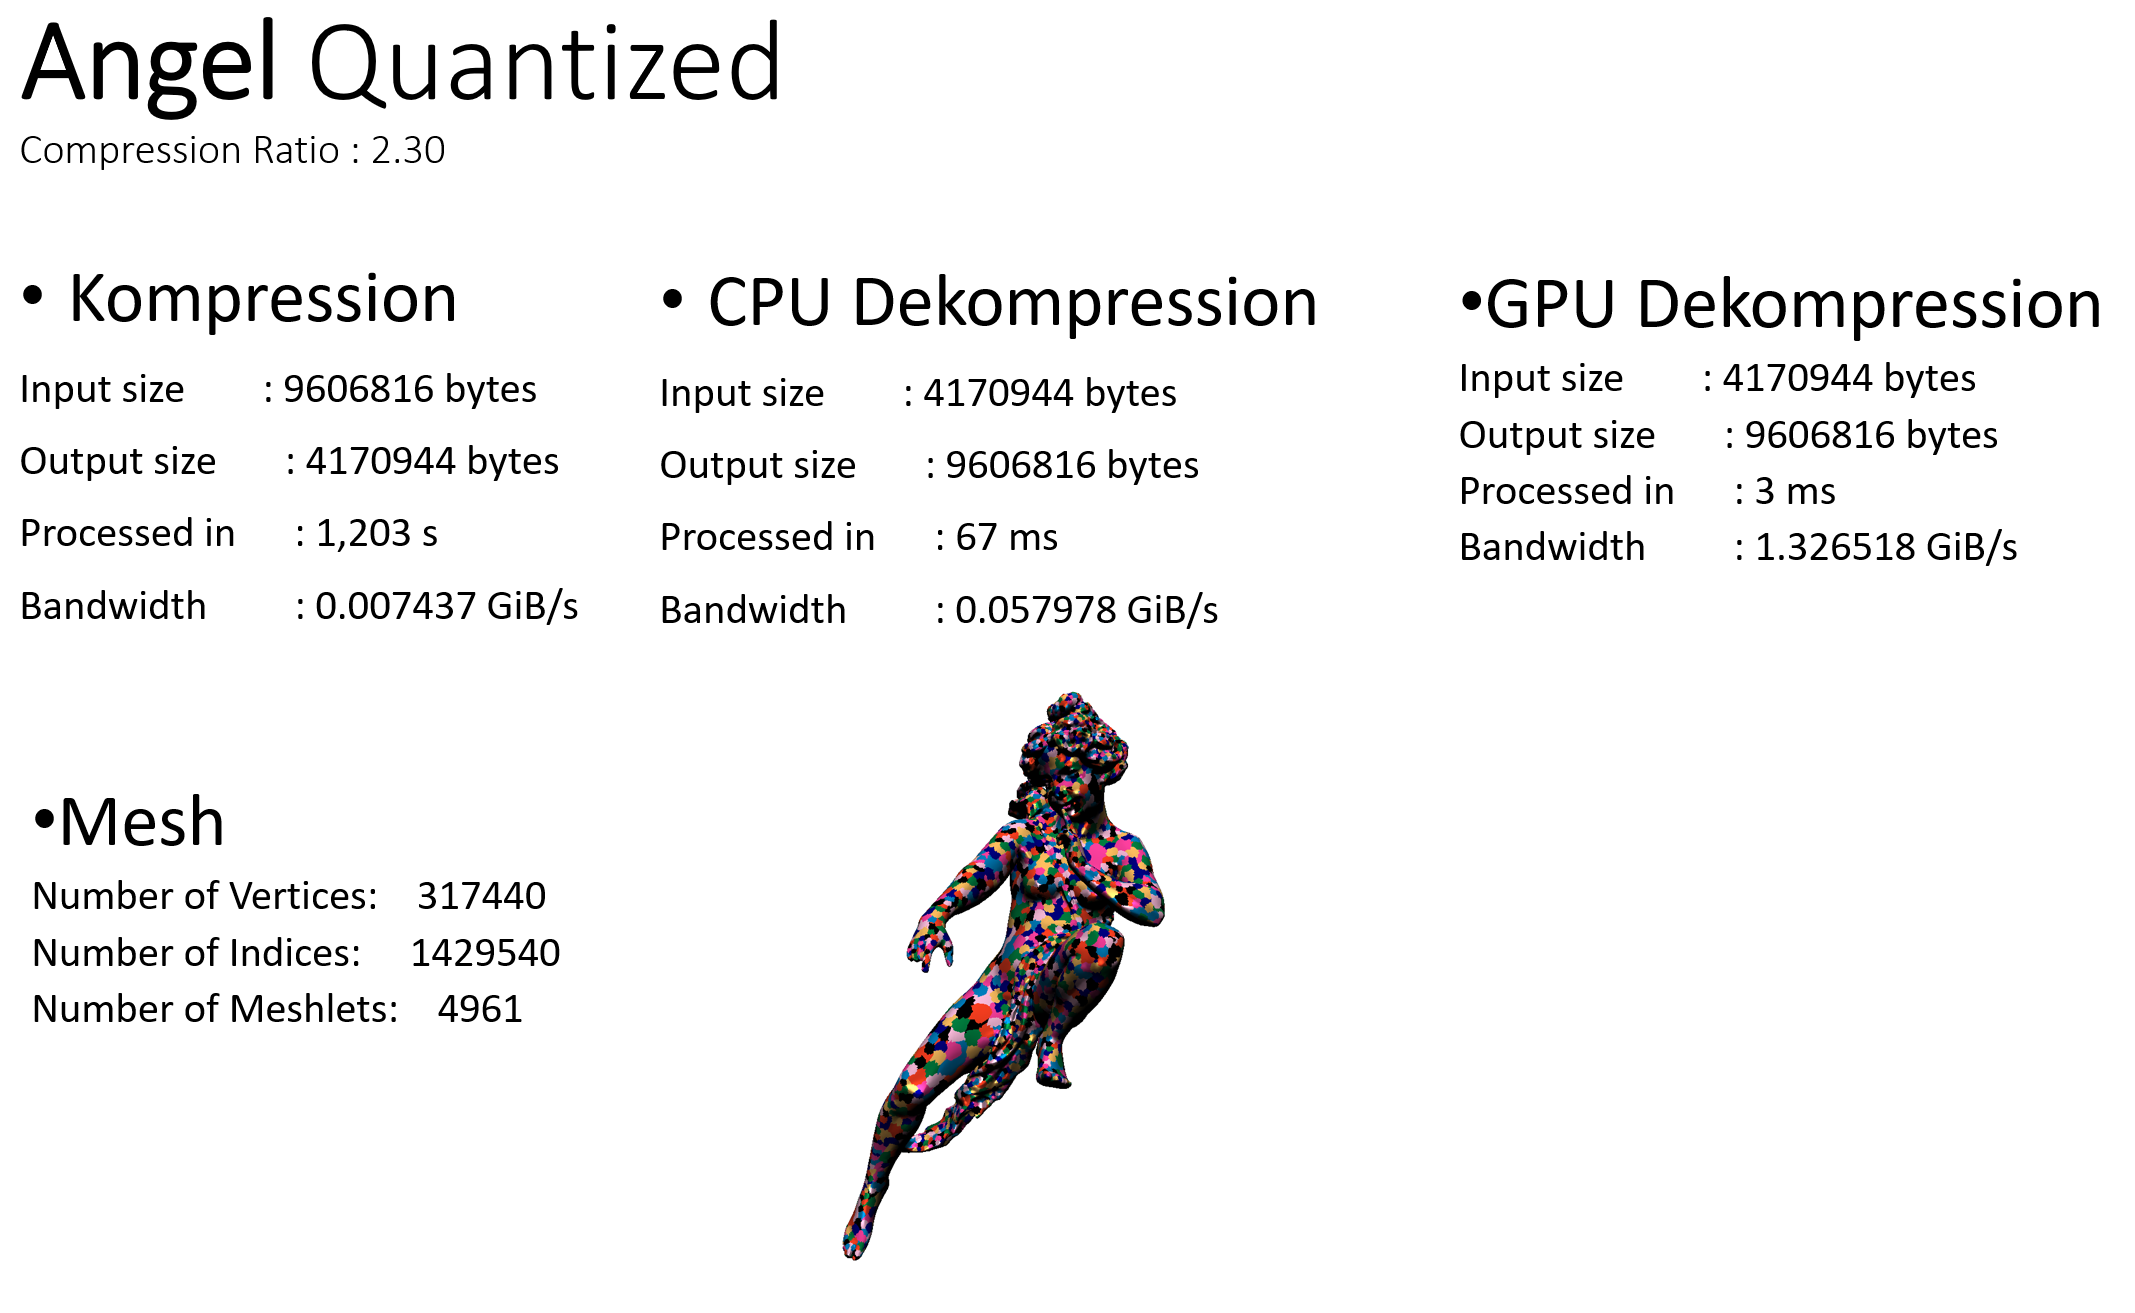
\includegraphics[scale=0.28]{Bilder/ergebnisse_full/angel_quantized.png}
\end{figure}
\begin{figure}[h]
  \centering  
  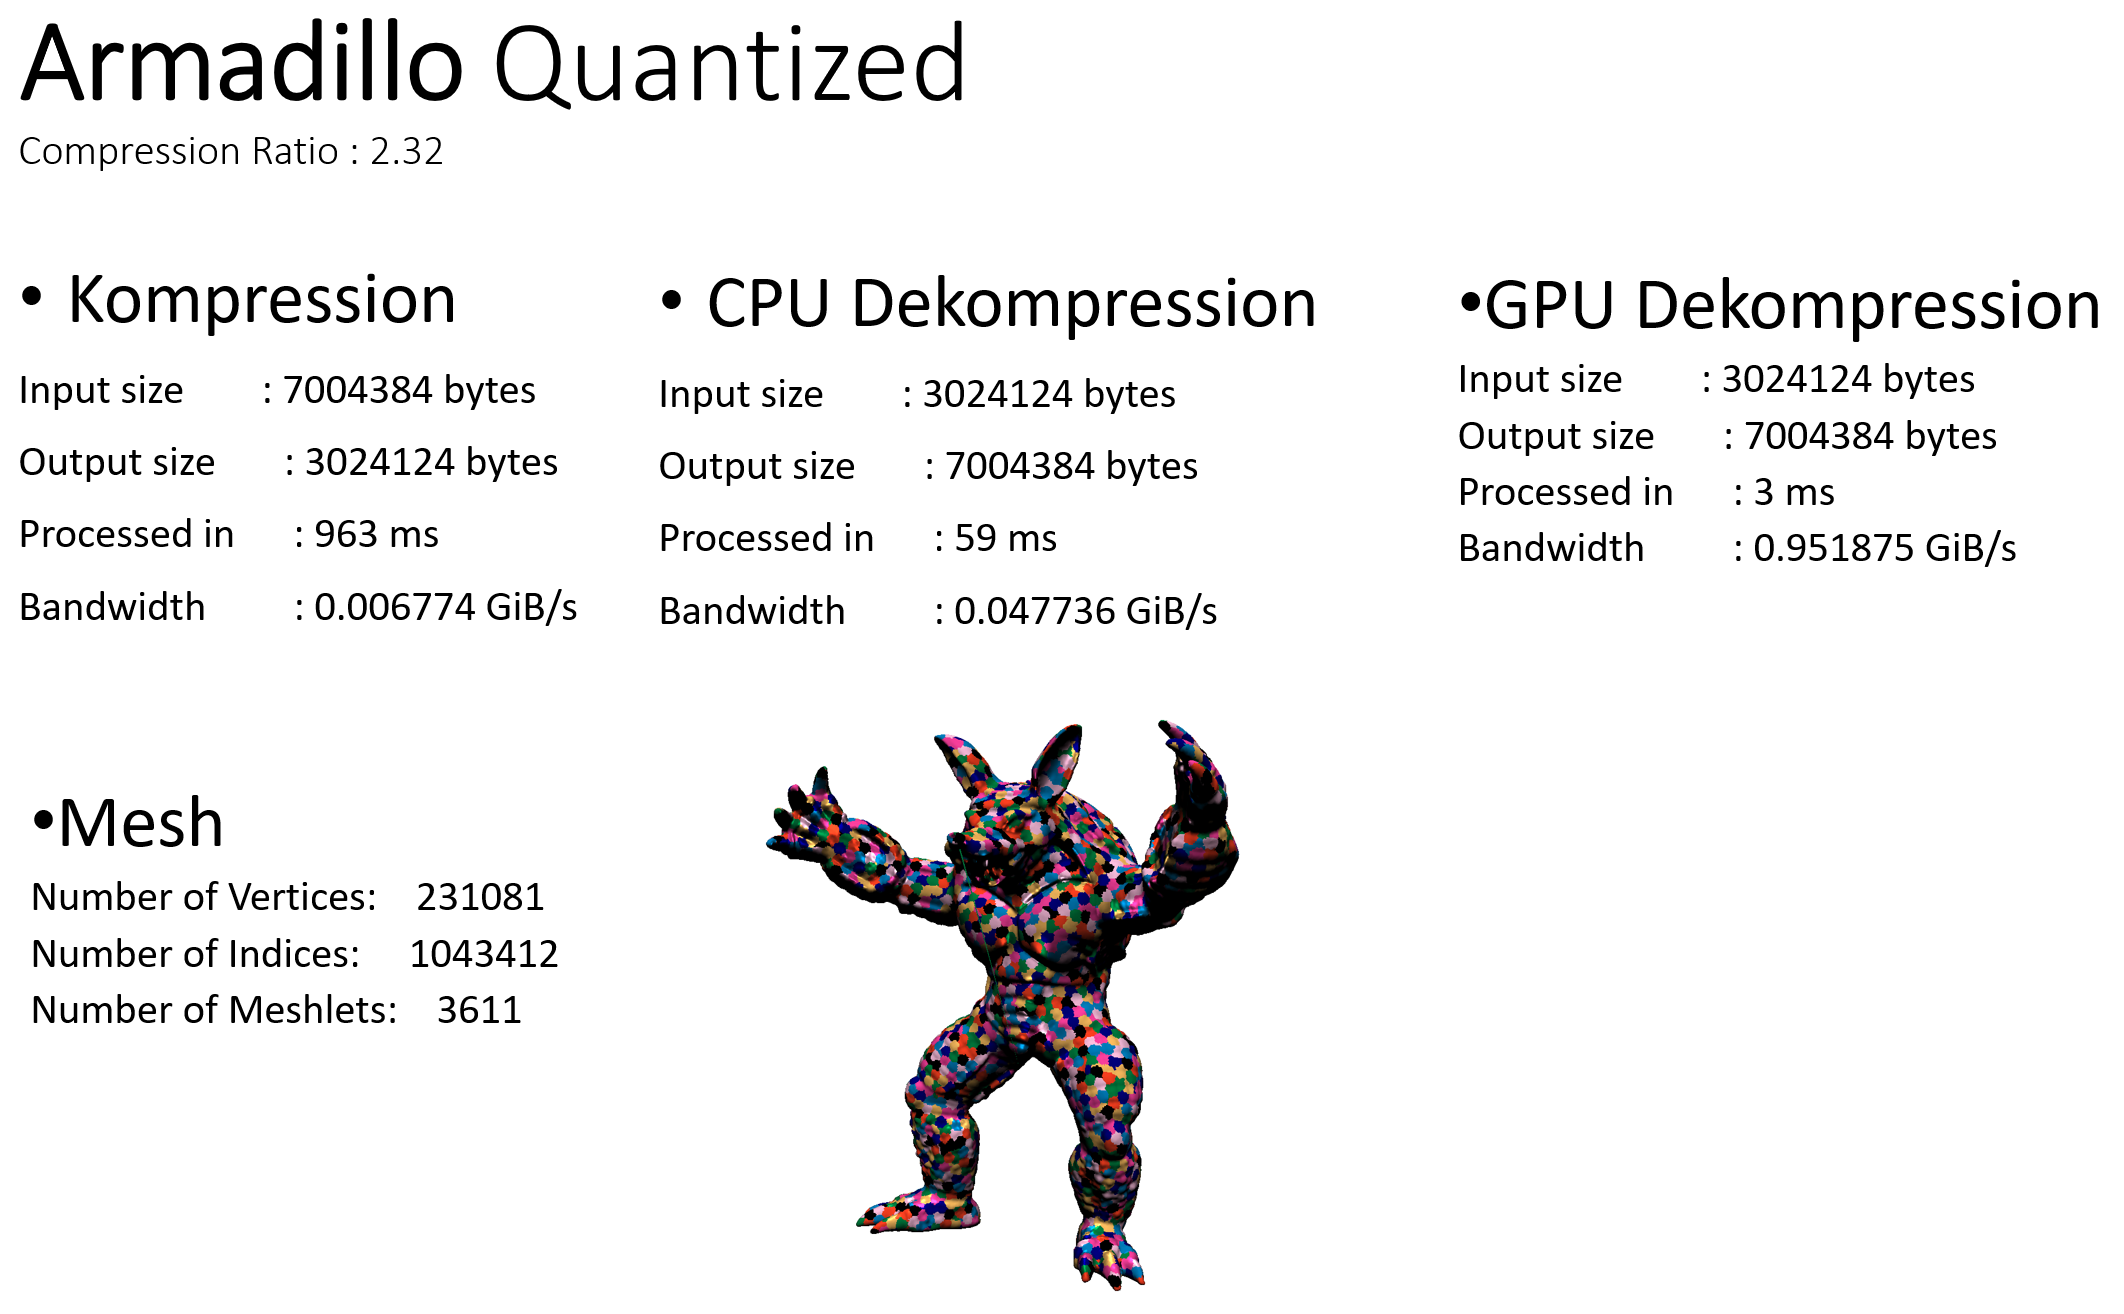
\includegraphics[scale=0.28]{Bilder/ergebnisse_full/armadillo_quantized.png}
\end{figure}
\begin{figure}[h]
  \centering  
  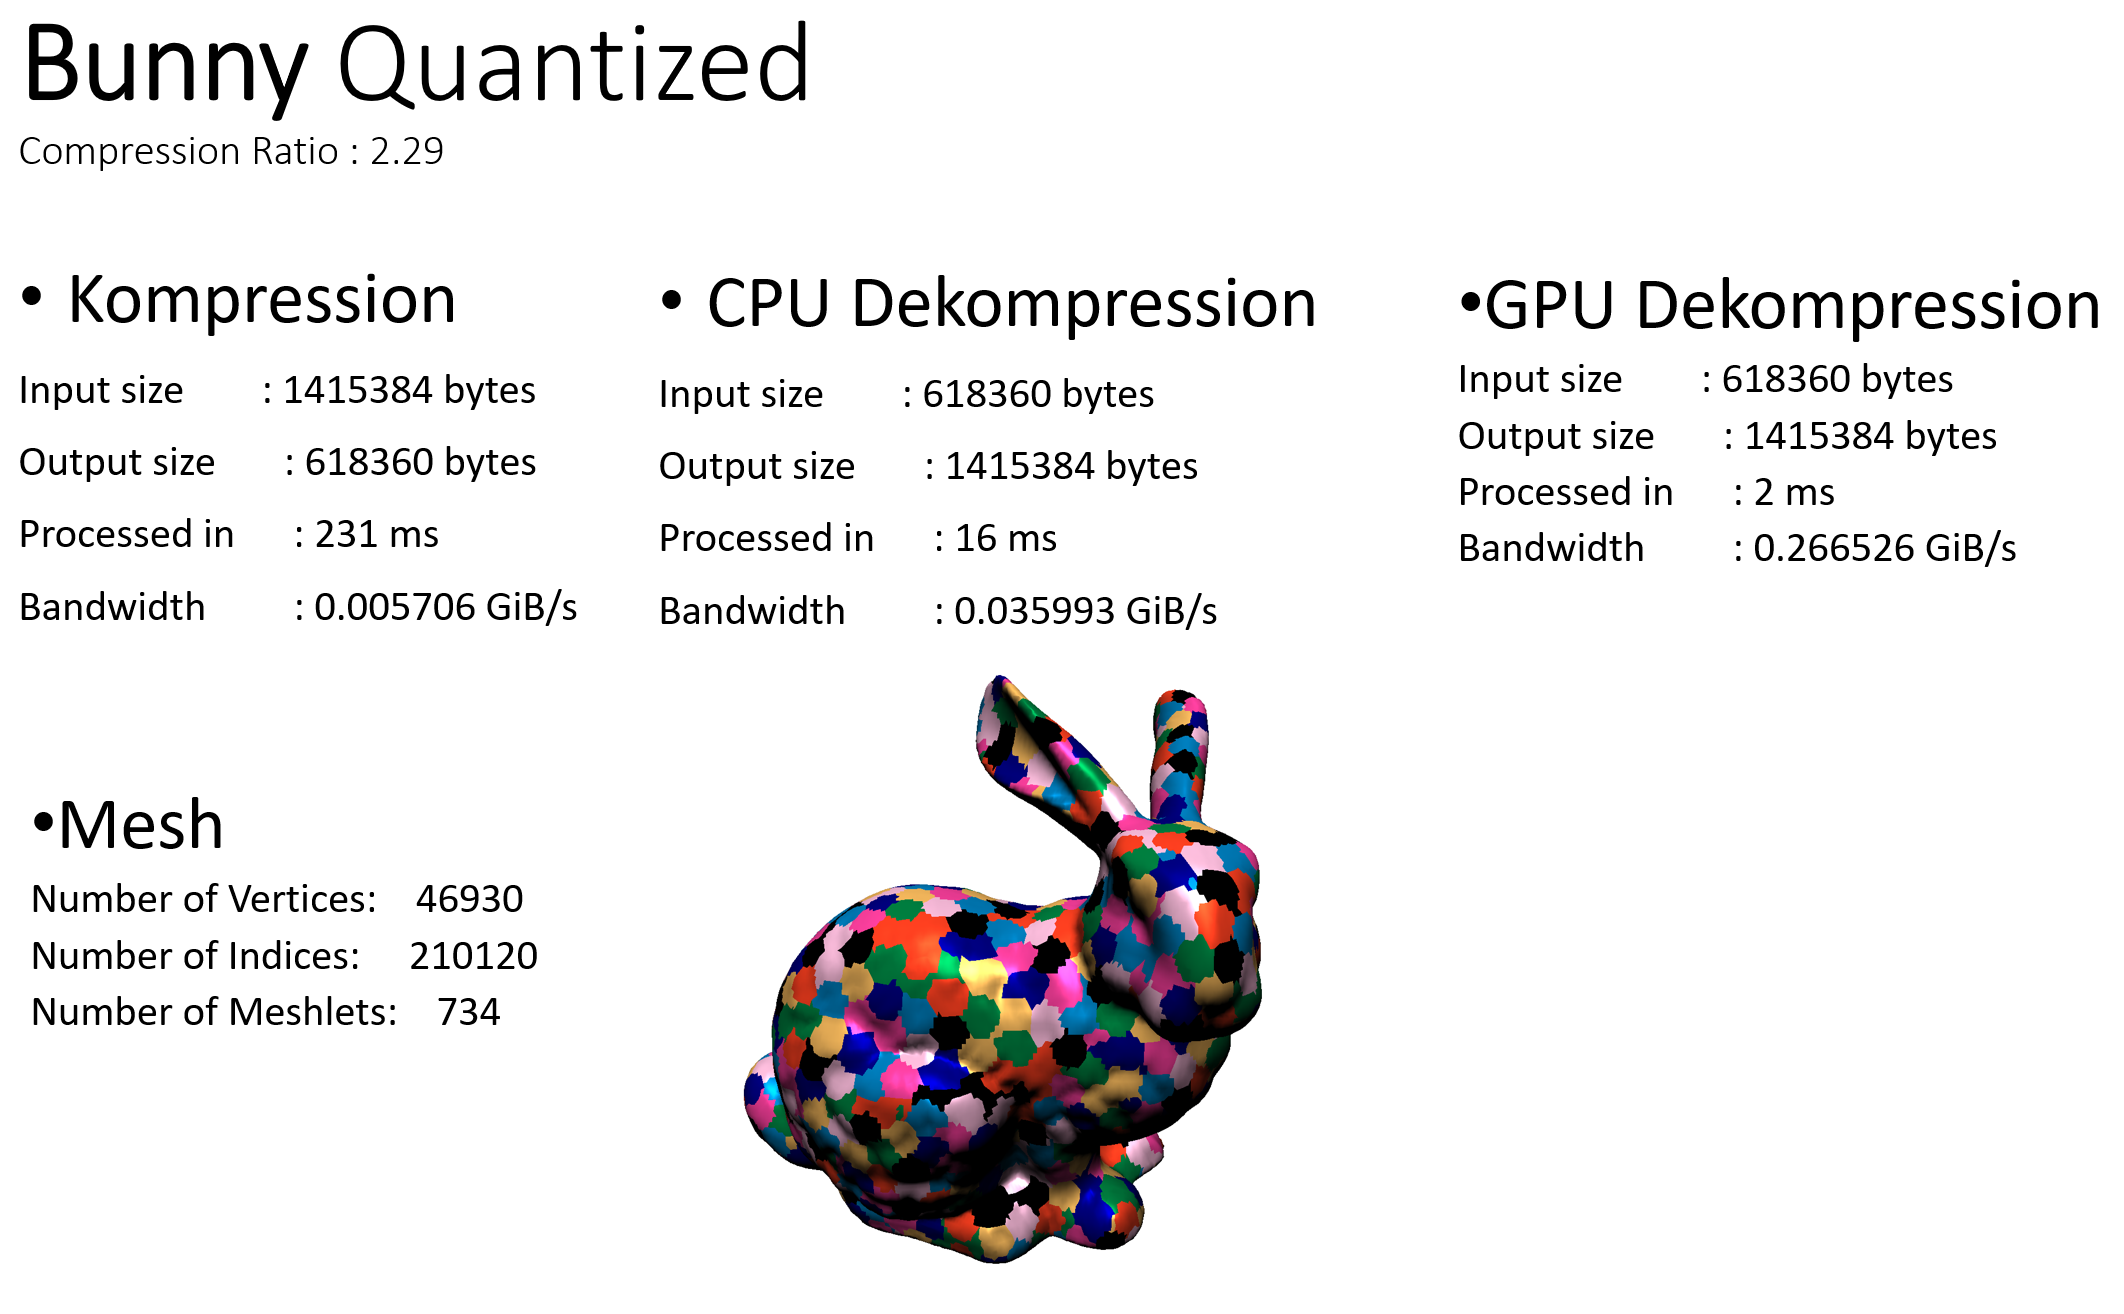
\includegraphics[scale=0.28]{Bilder/ergebnisse_full/bunny_quantized.png}
\end{figure}
\begin{figure}[h]
  \centering  
  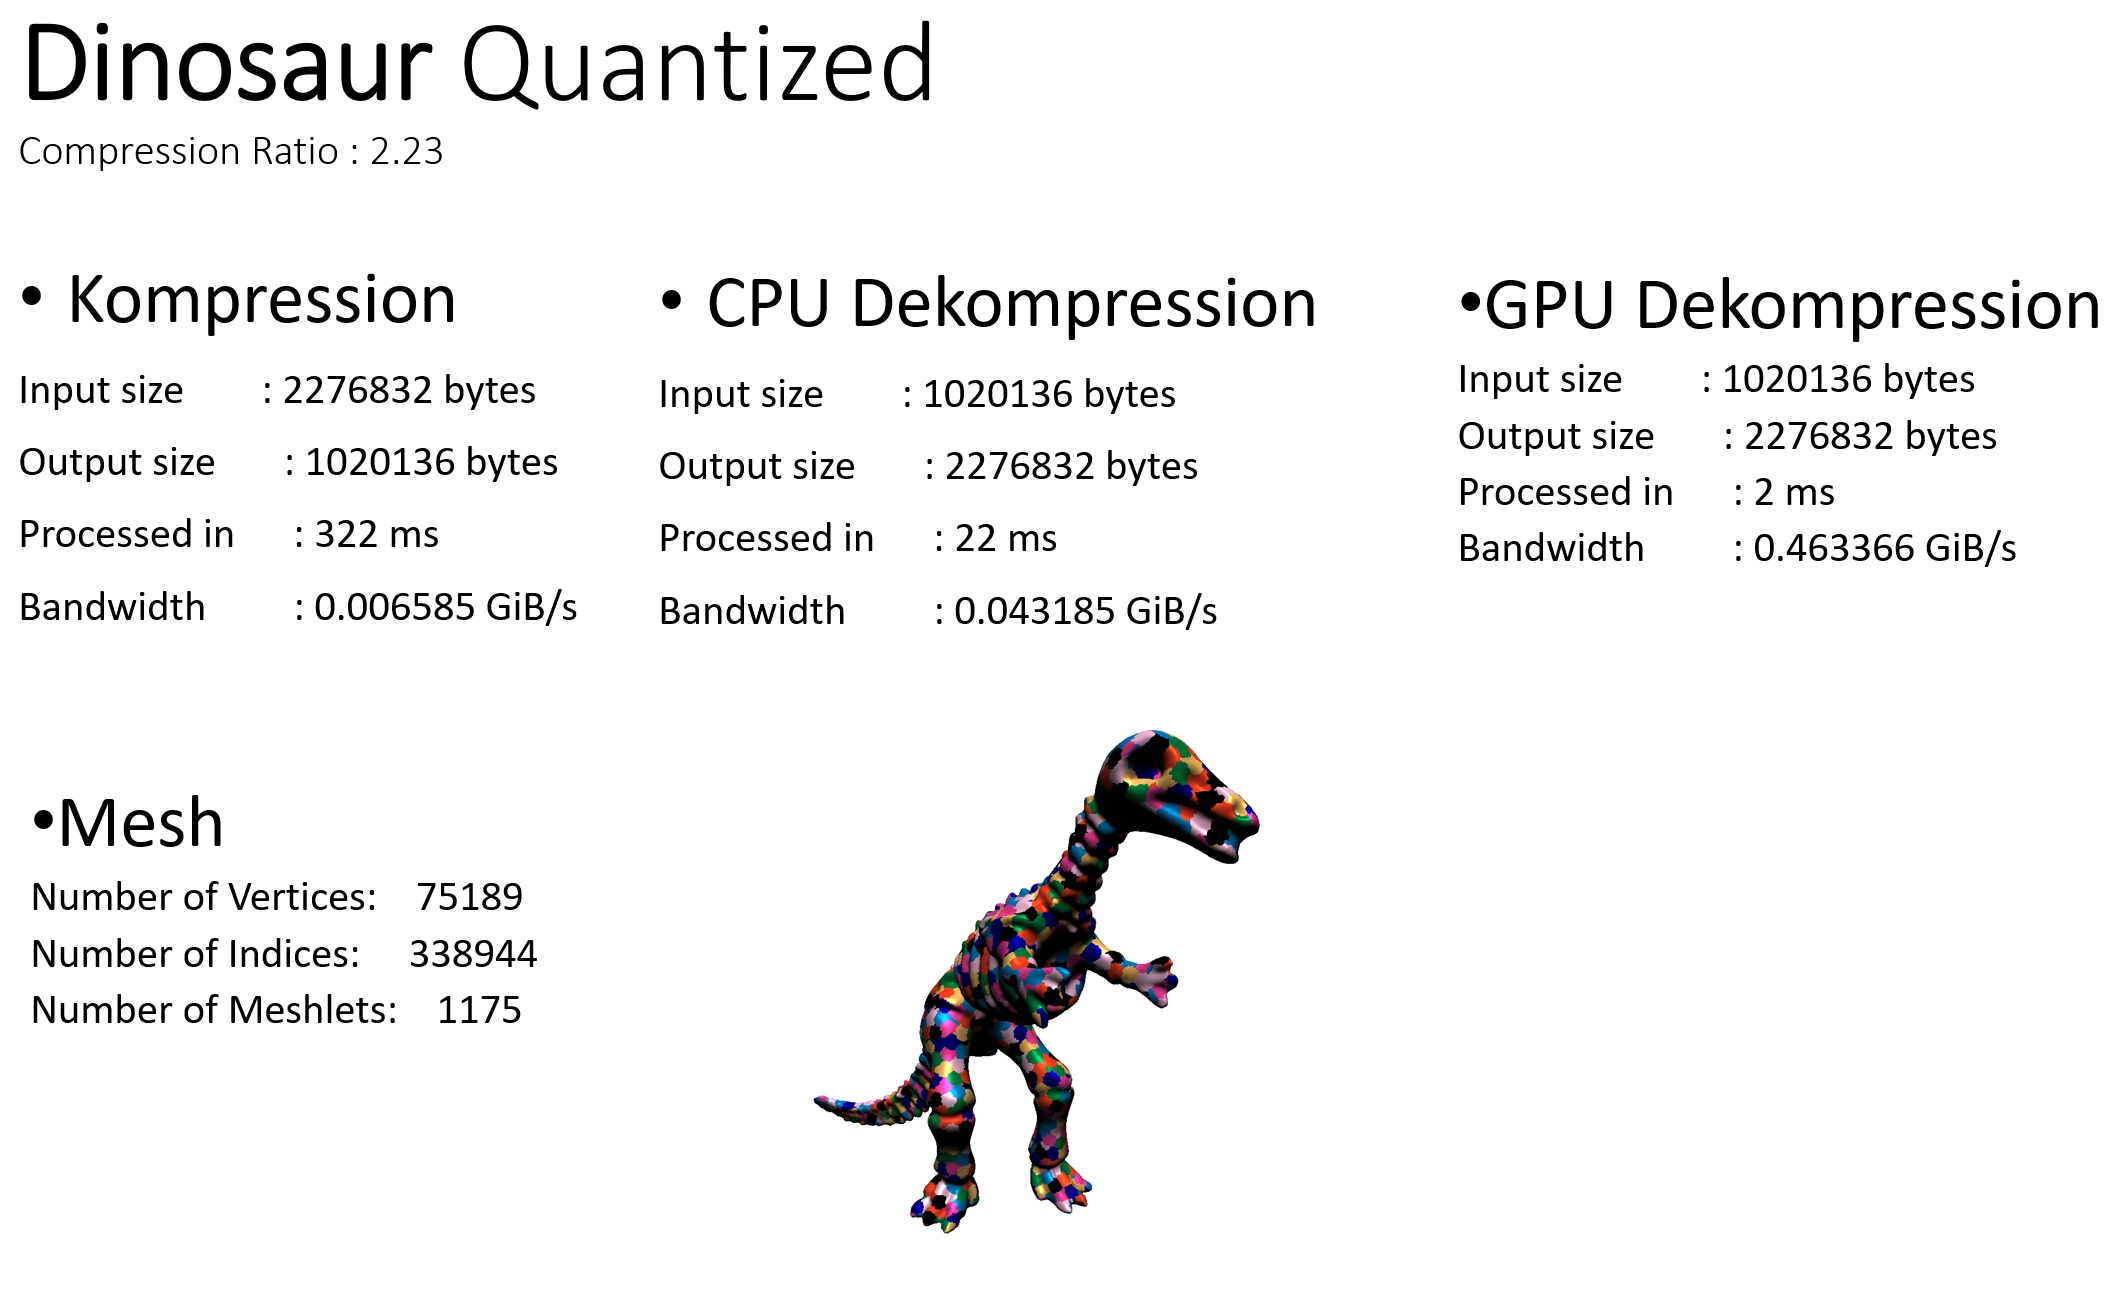
\includegraphics[scale=0.28]{Bilder/ergebnisse_full/dinosaur_quantized.png}
\end{figure}
\begin{figure}[h]
  \centering  
  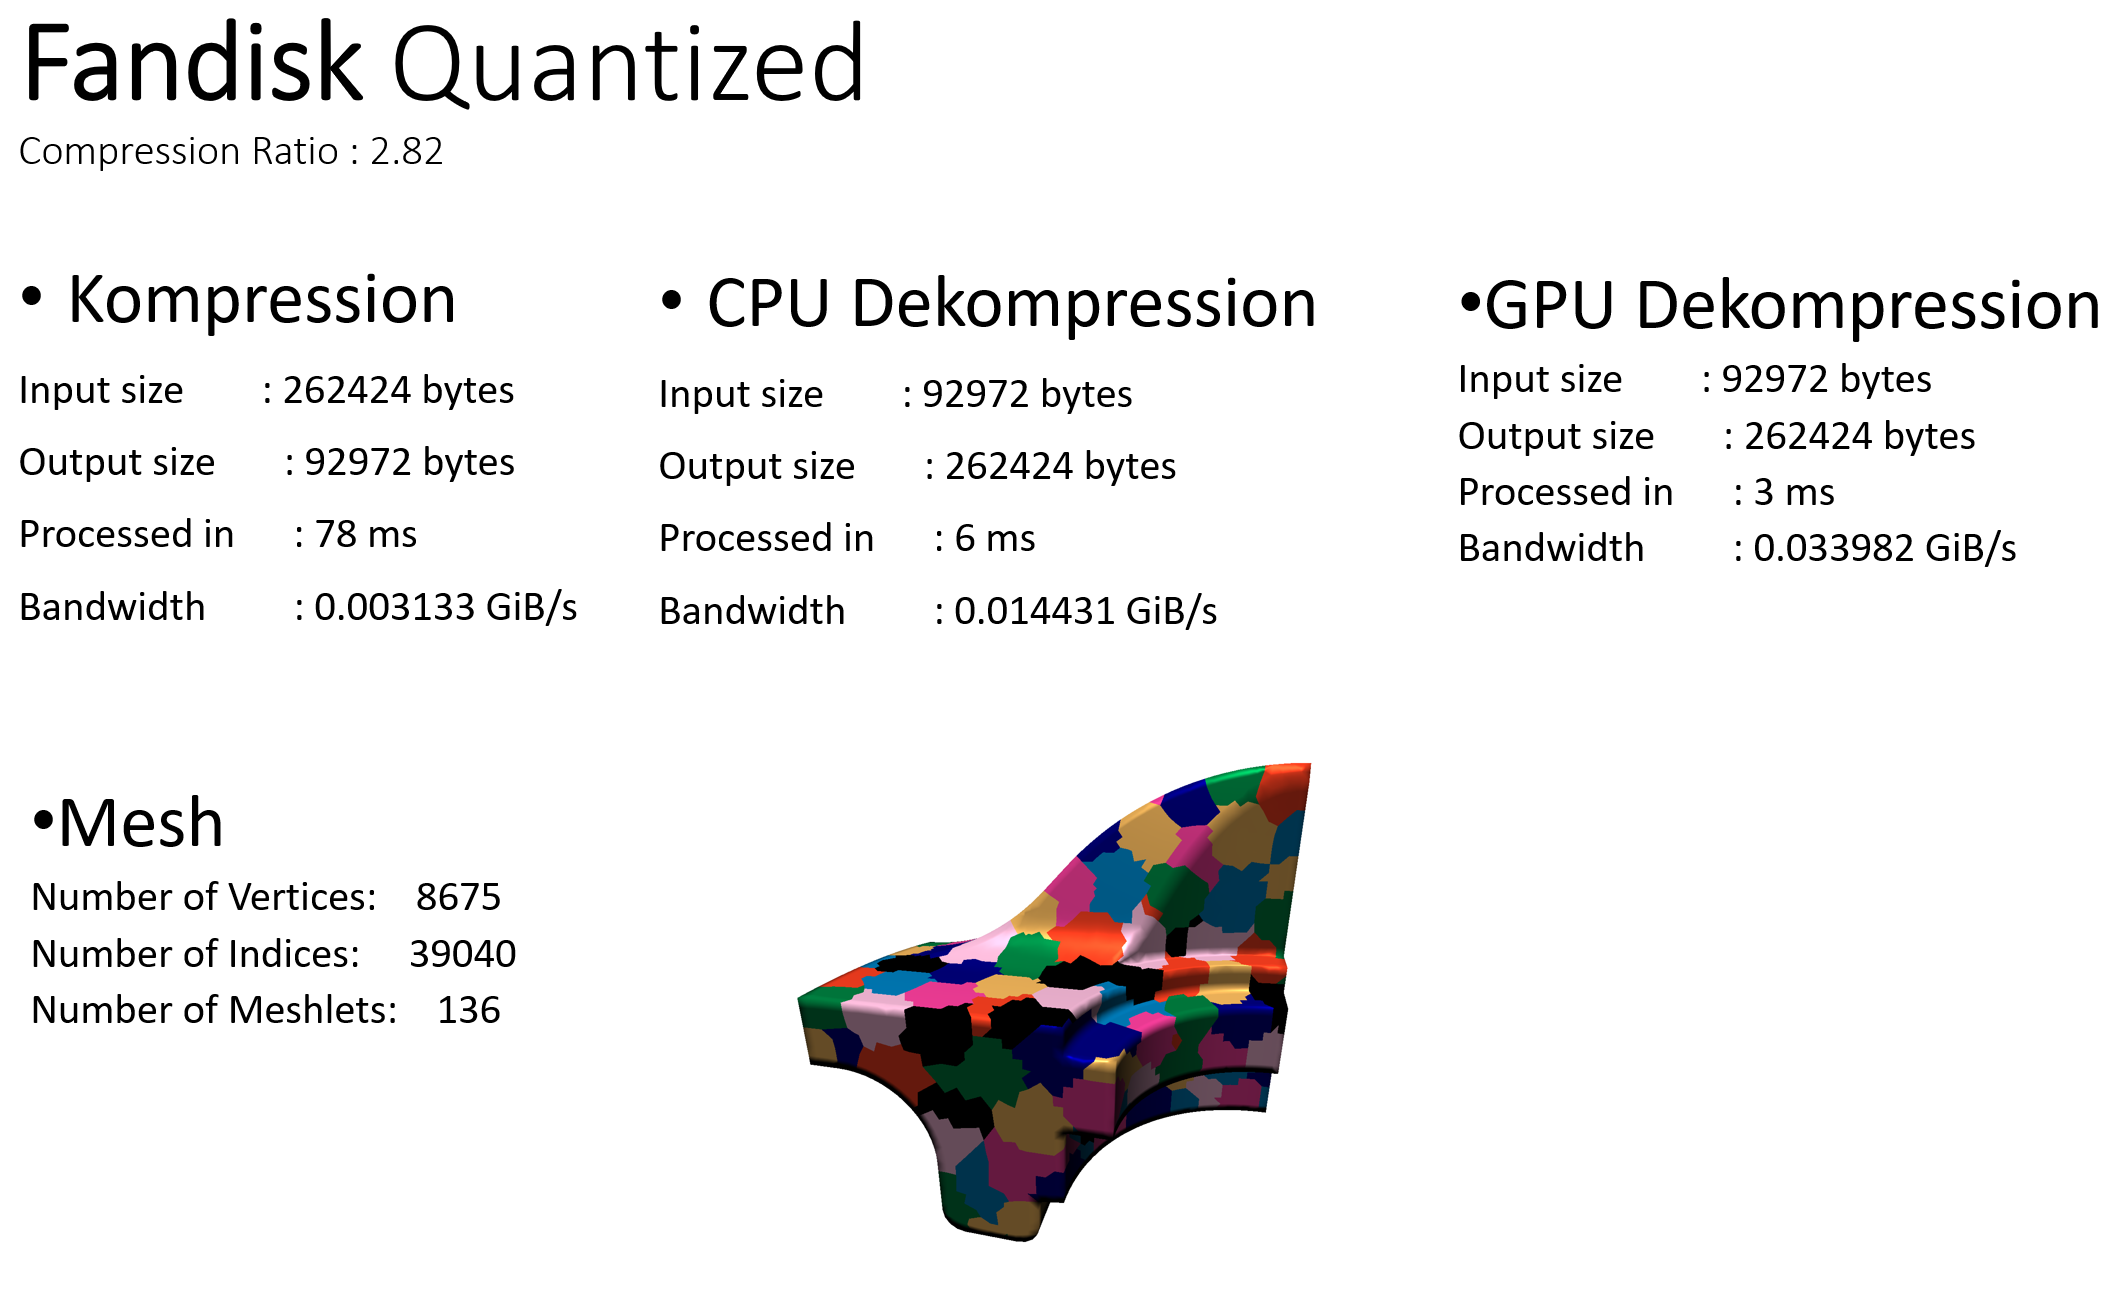
\includegraphics[scale=0.28]{Bilder/ergebnisse_full/fandisk_quantized.png}
\end{figure}
\begin{figure}[h]
  \centering  
  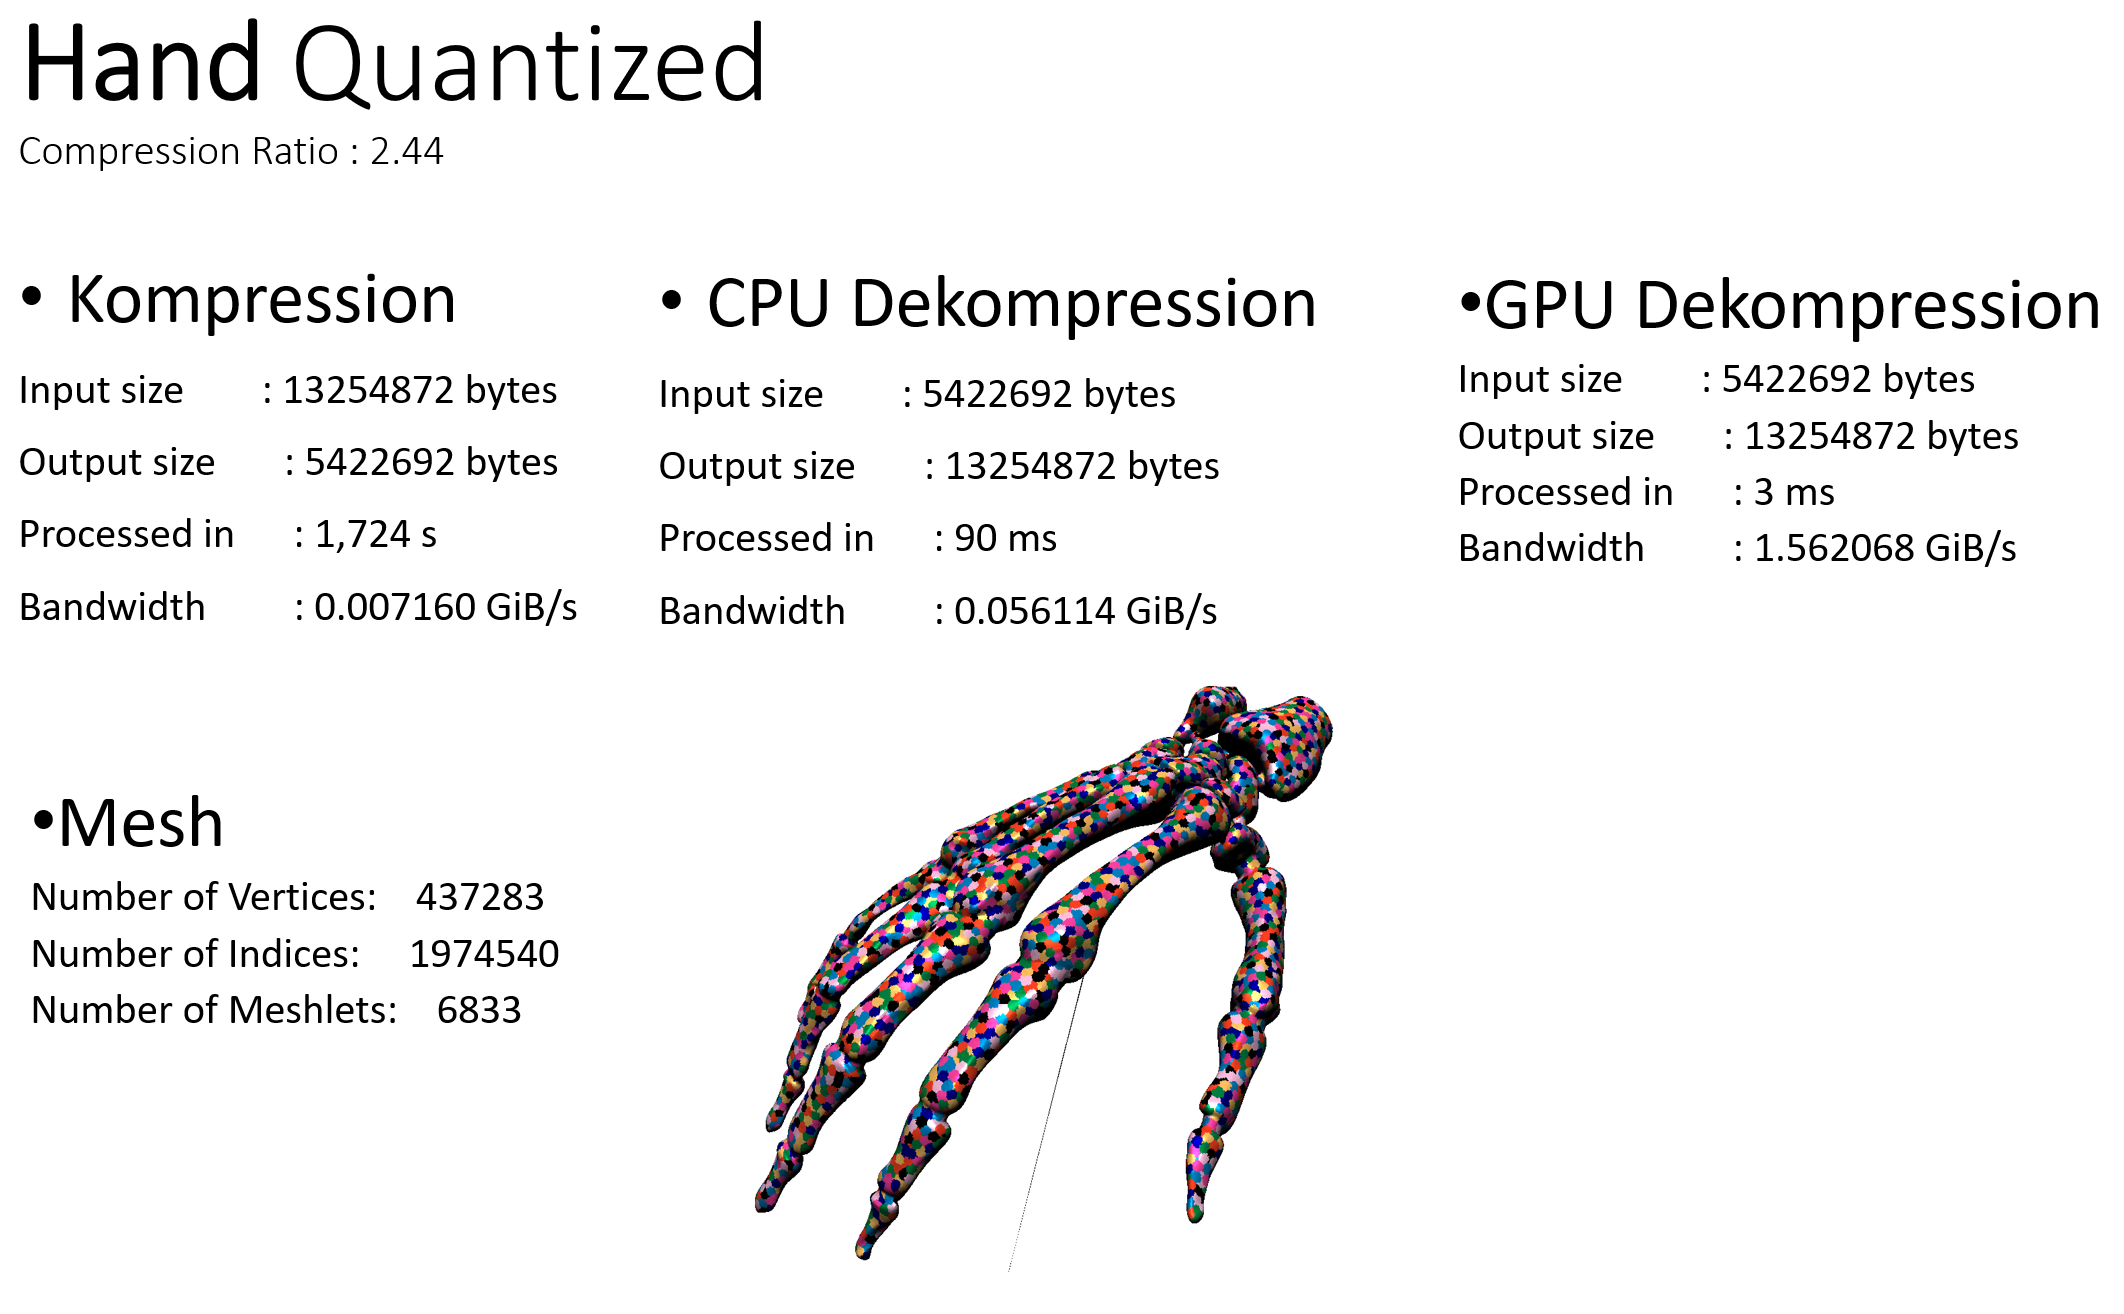
\includegraphics[scale=0.28]{Bilder/ergebnisse_full/hand_quantized.png}
\end{figure}
\begin{figure}[h]
  \centering  
  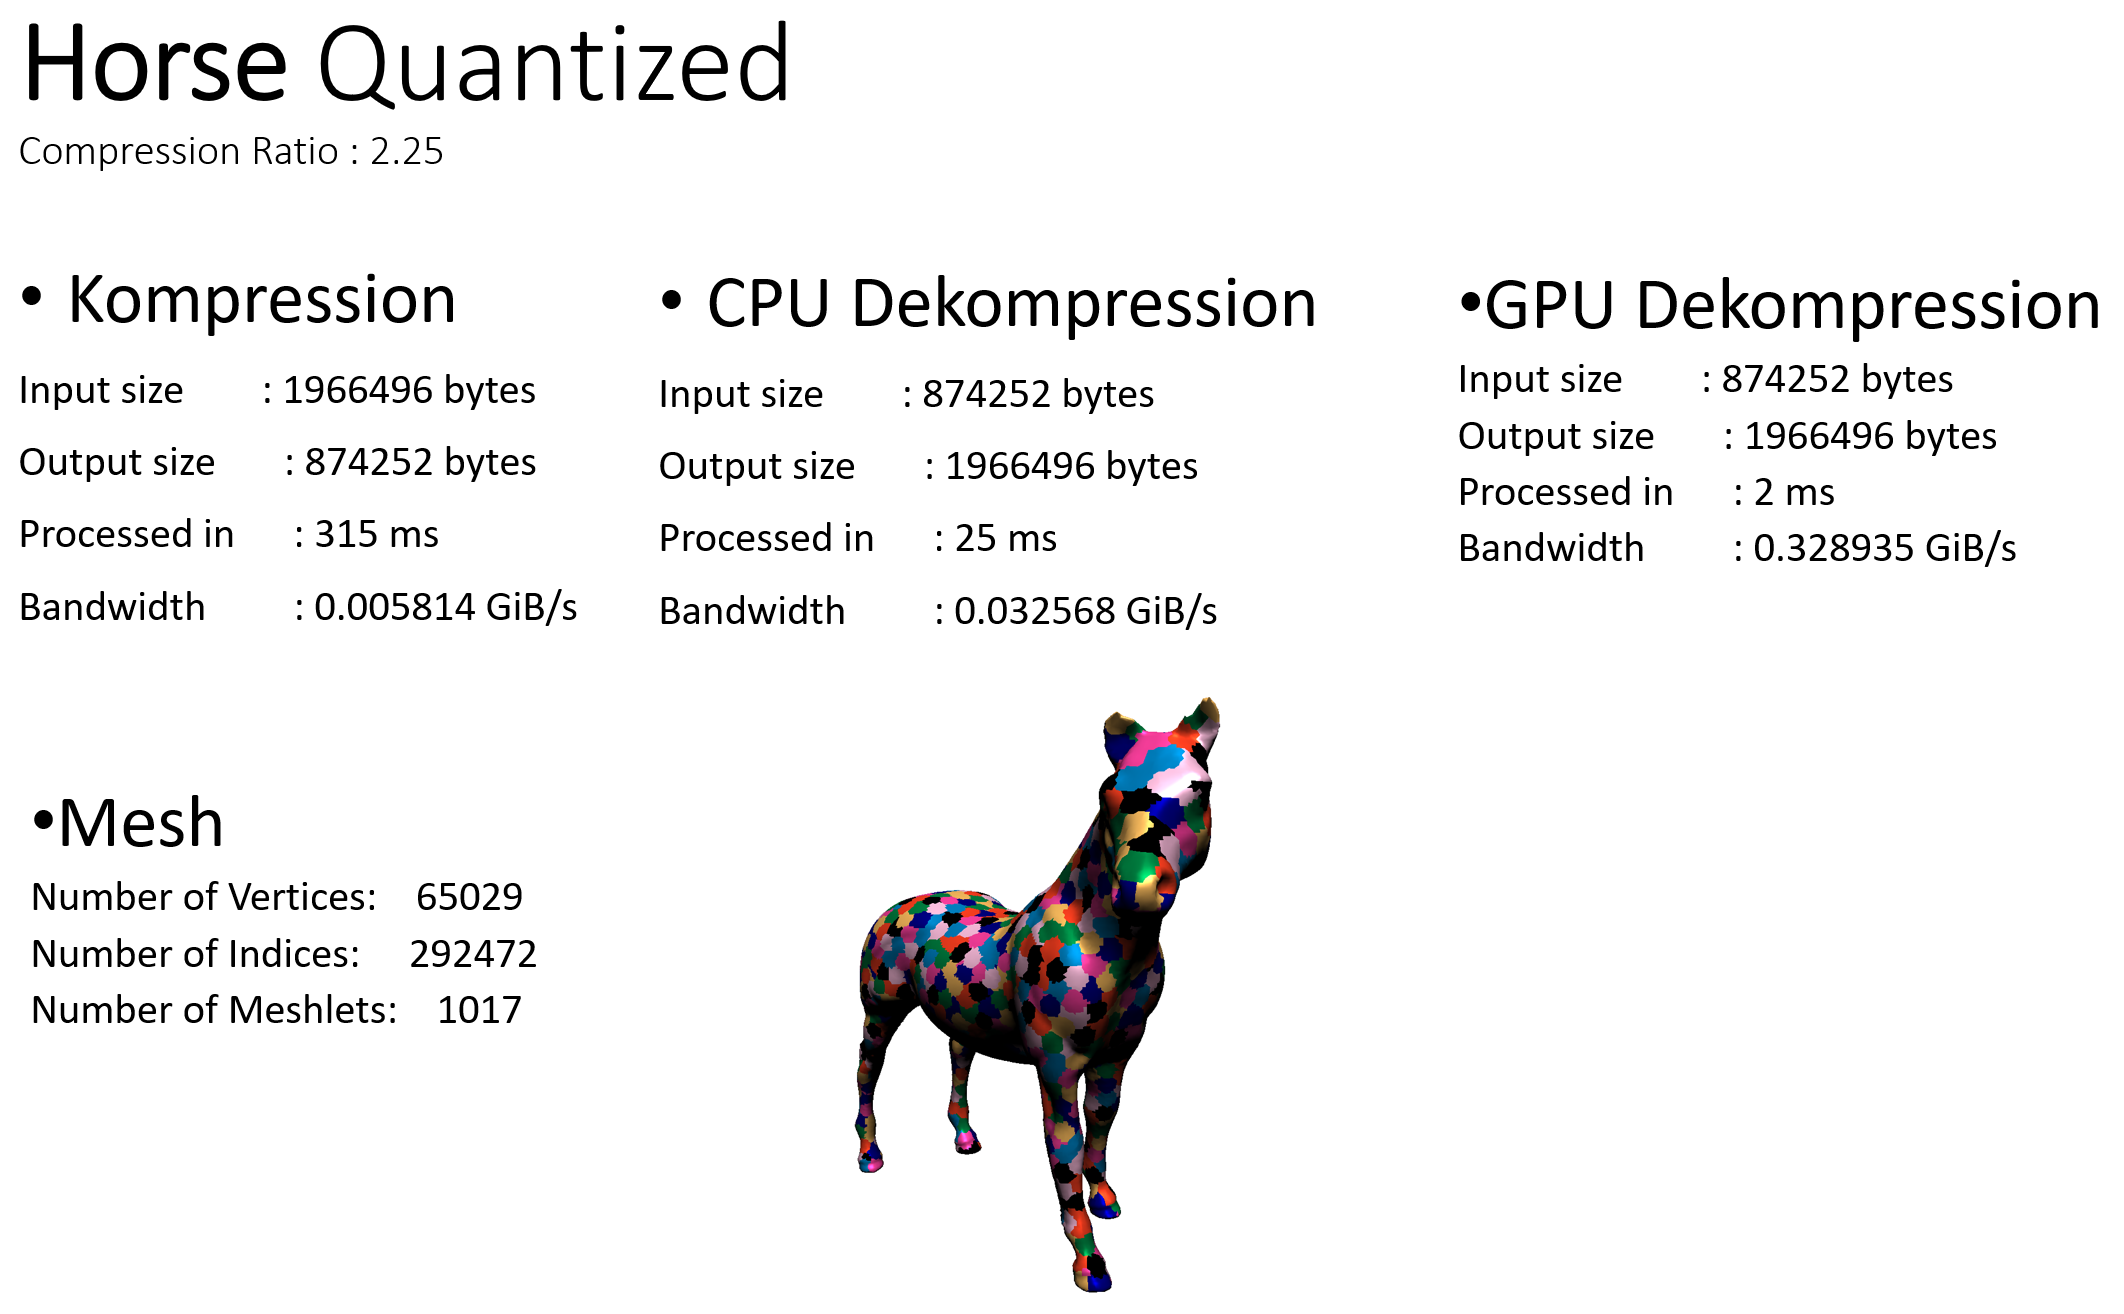
\includegraphics[scale=0.28]{Bilder/ergebnisse_full/horse_quantized.png}
\end{figure}
\begin{figure}[h]
  \centering  
  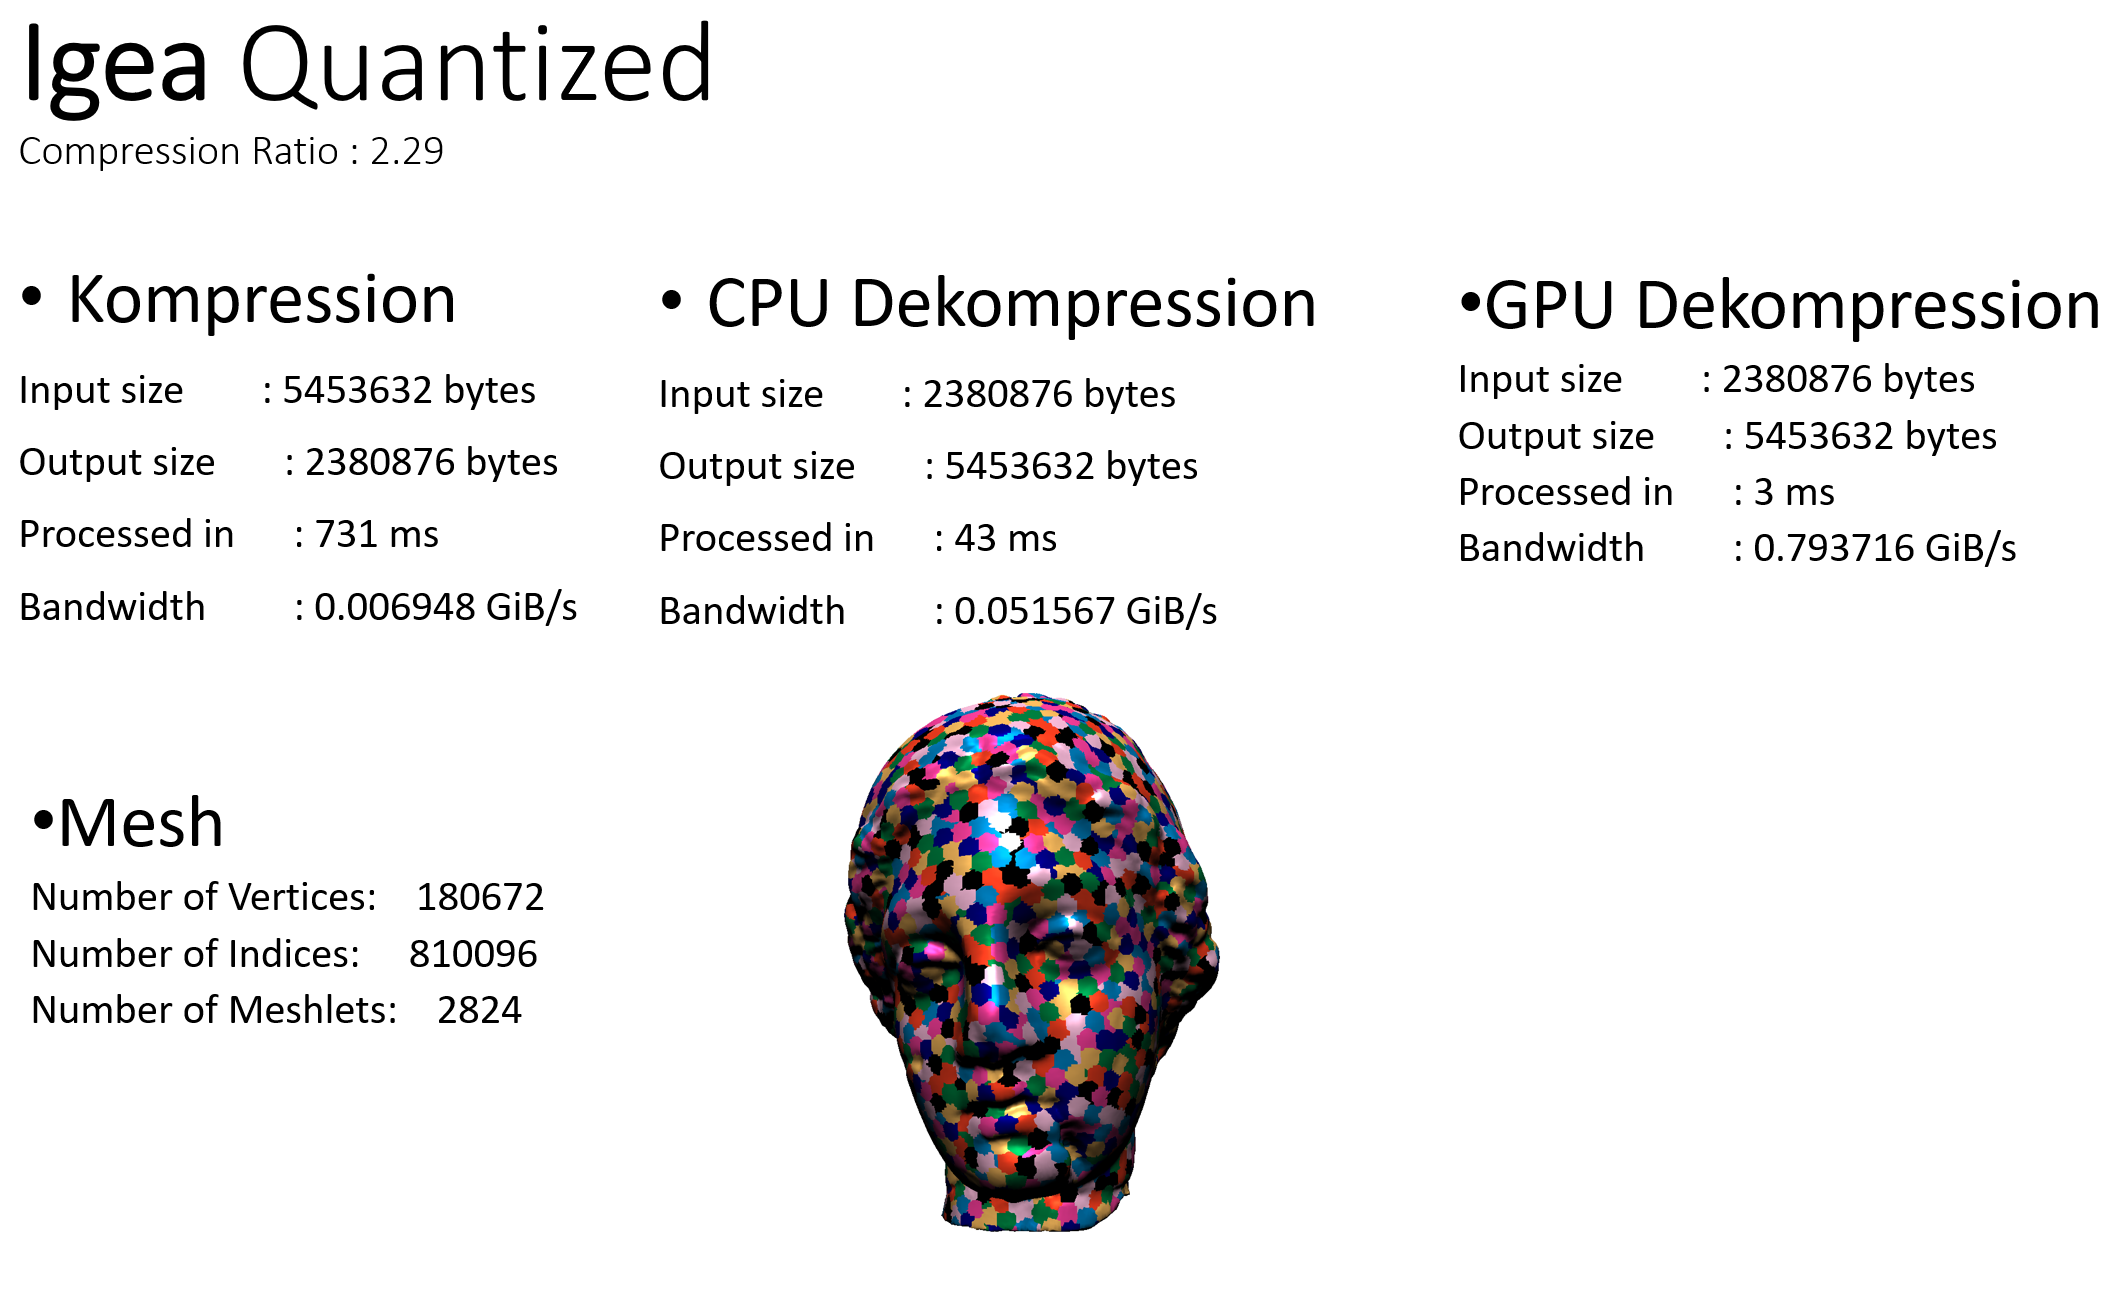
\includegraphics[scale=0.28]{Bilder/ergebnisse_full/igea_quantized.png}
\end{figure}
\begin{figure}[h]
  \centering  
  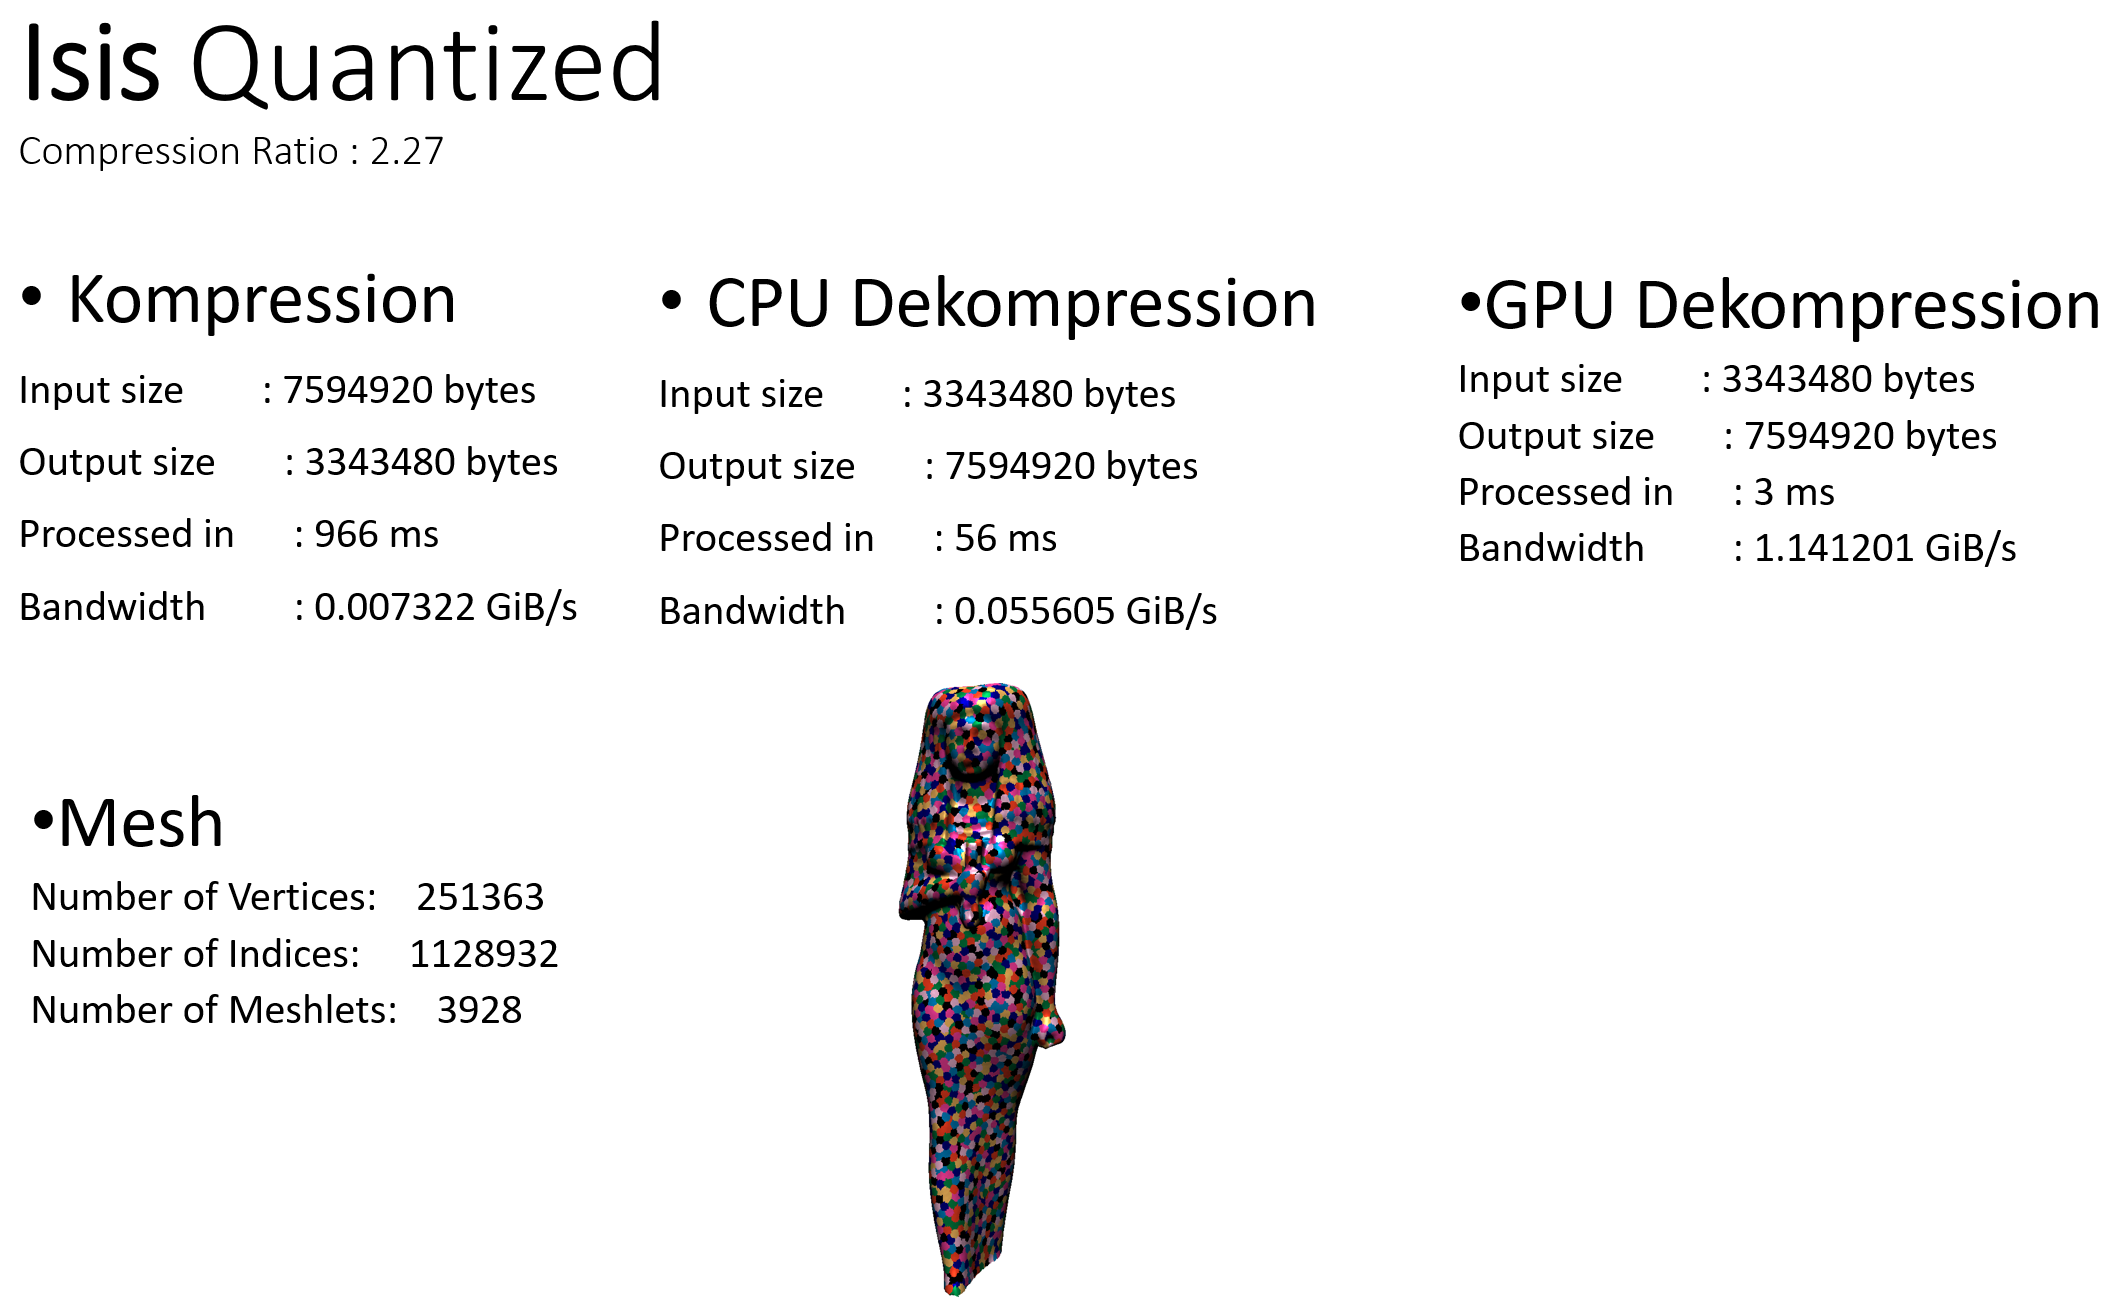
\includegraphics[scale=0.28]{Bilder/ergebnisse_full/isis_quantized.png}
\end{figure}
\begin{figure}[h]
  \centering  
  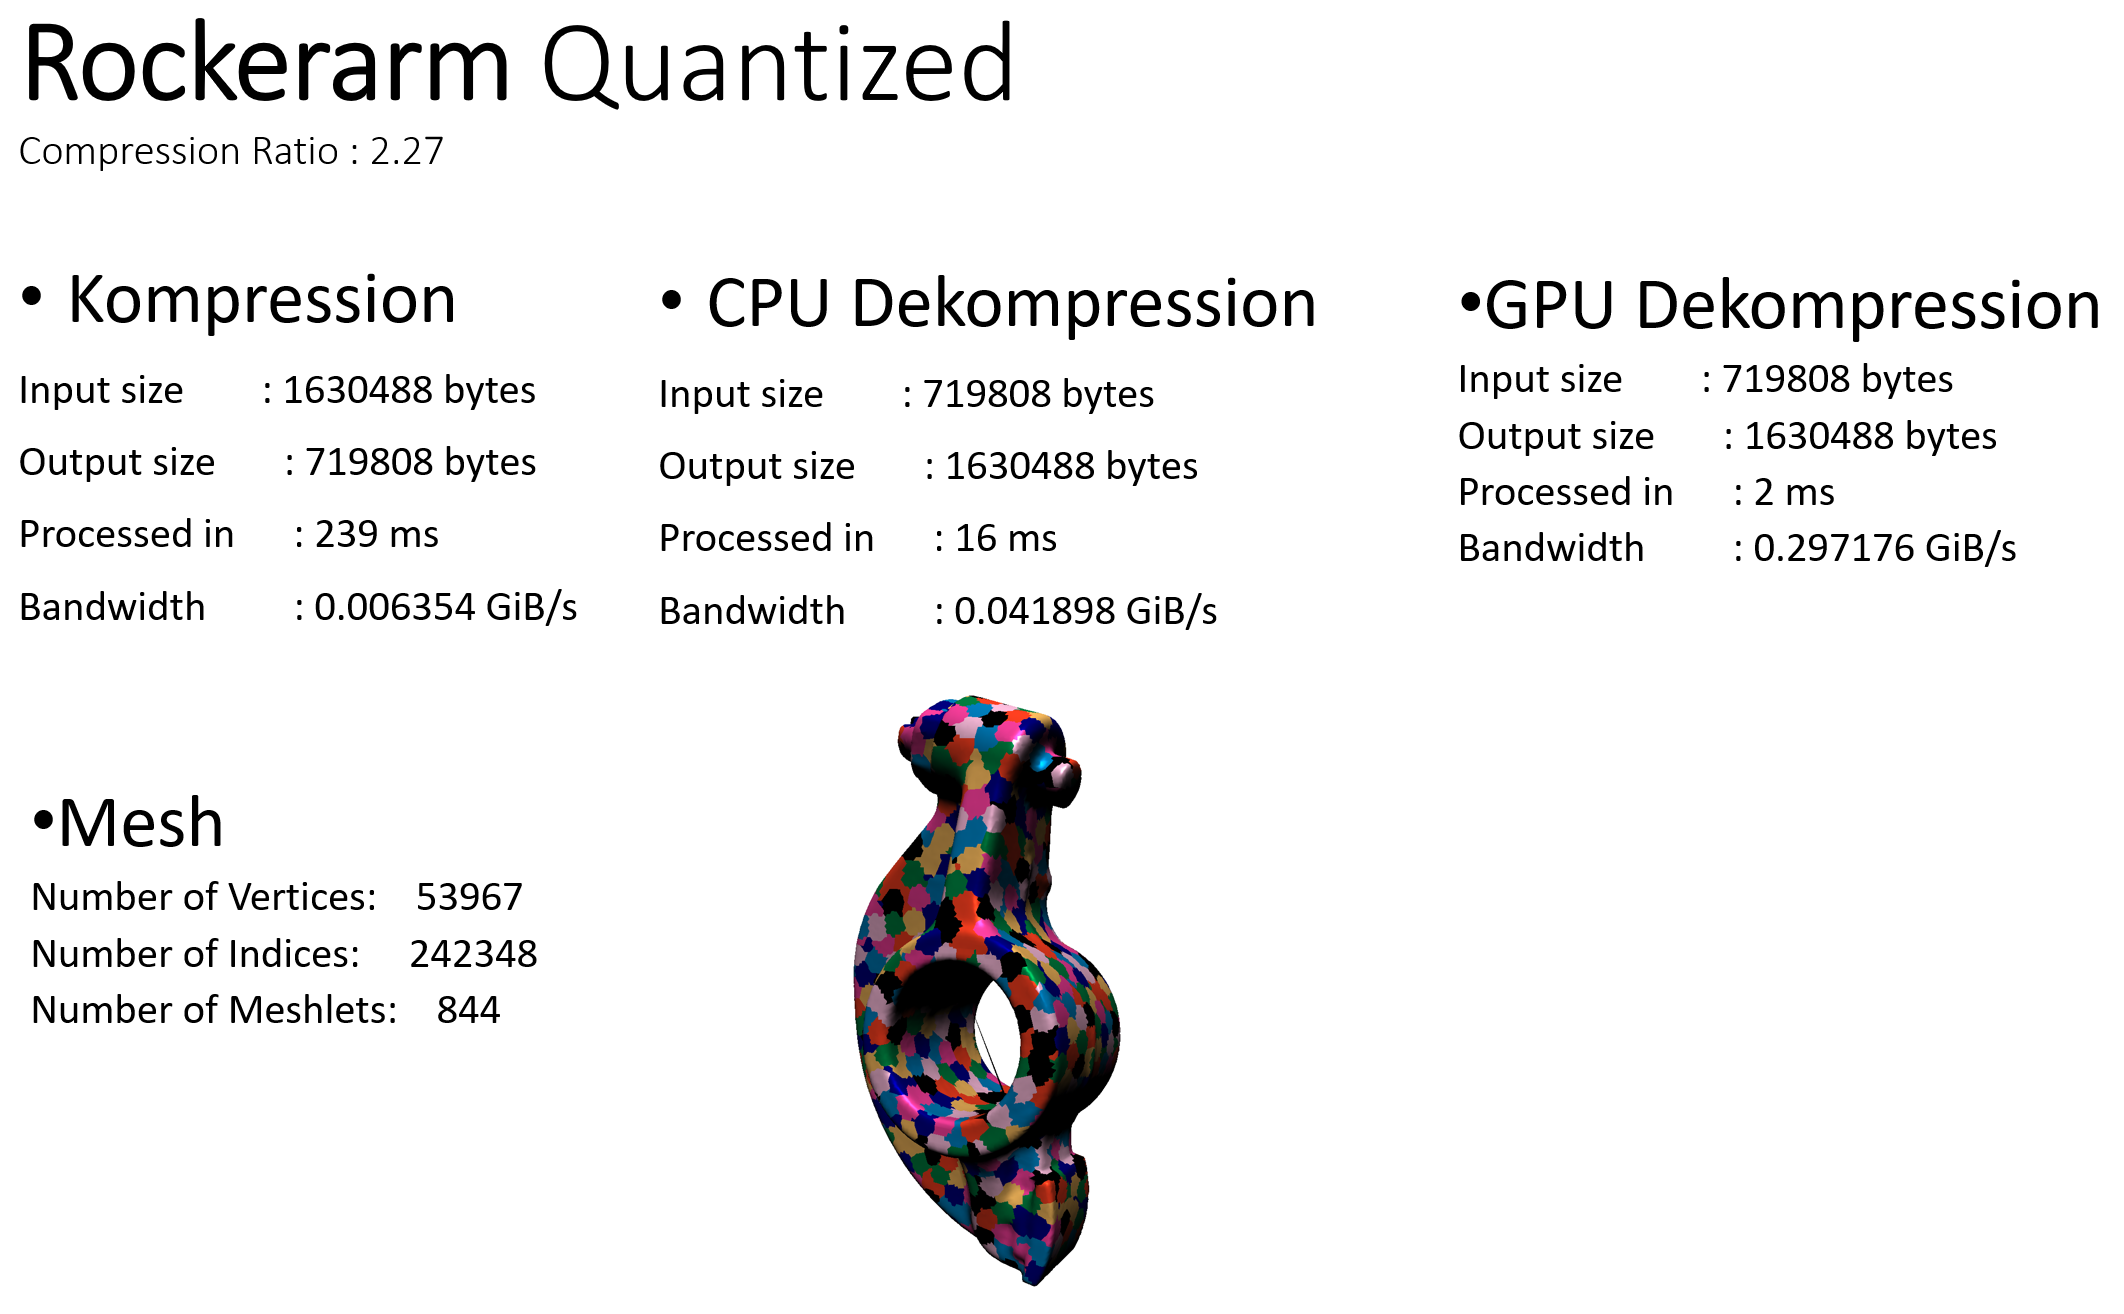
\includegraphics[scale=0.28]{Bilder/ergebnisse_full/rockerarm_quantized.png}
\end{figure}
\begin{figure}[h]
  \centering  
  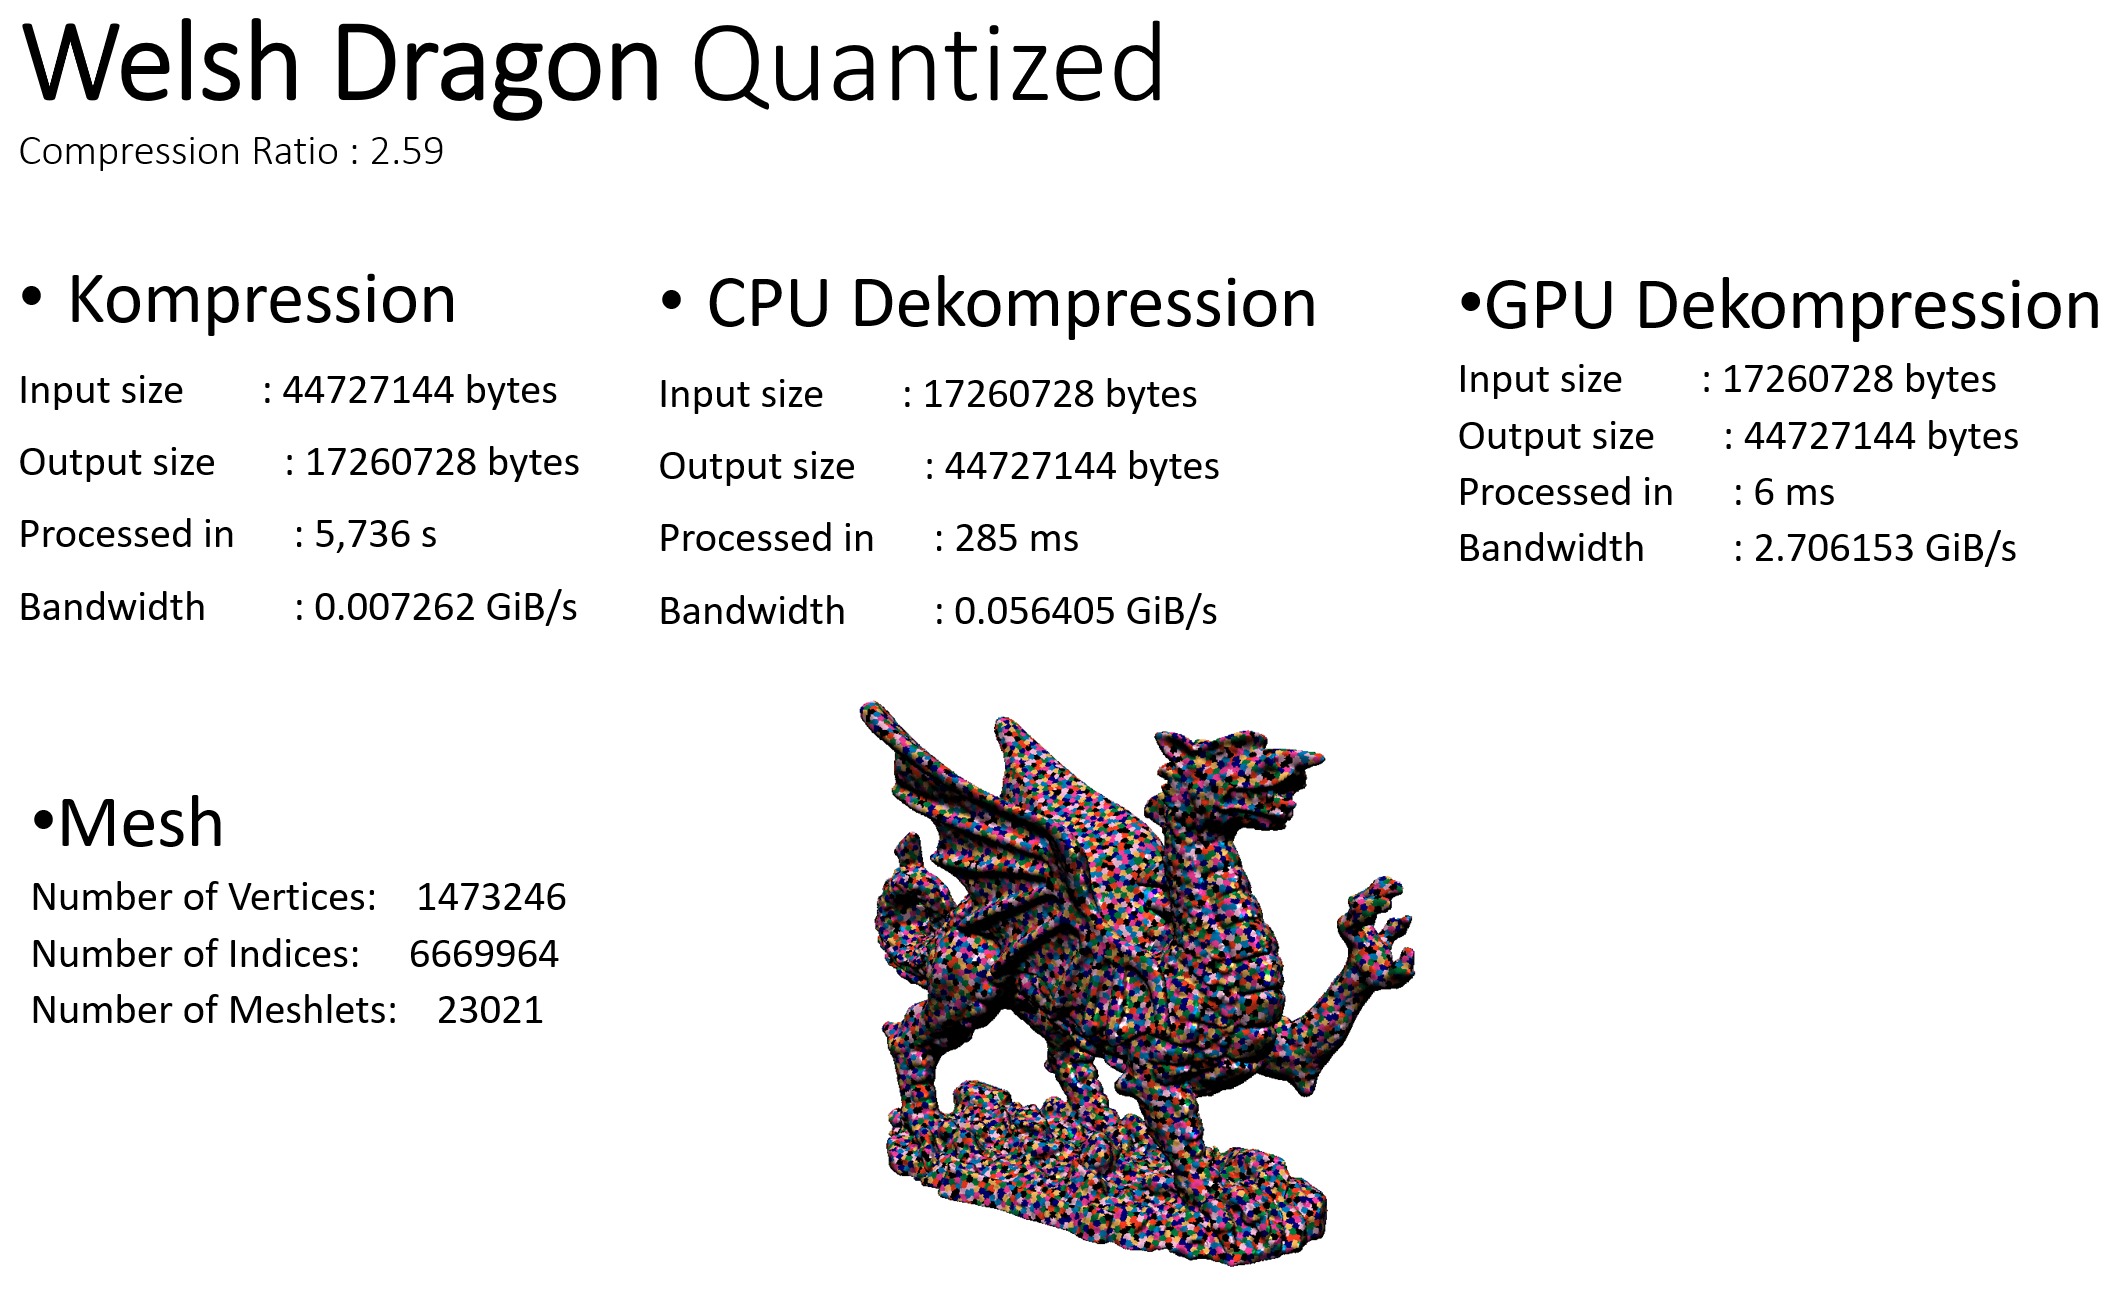
\includegraphics[scale=0.28]{Bilder/ergebnisse_full/welshdragon_quantized.png}
\end{figure}
\begin{figure}[h]
  \centering  
  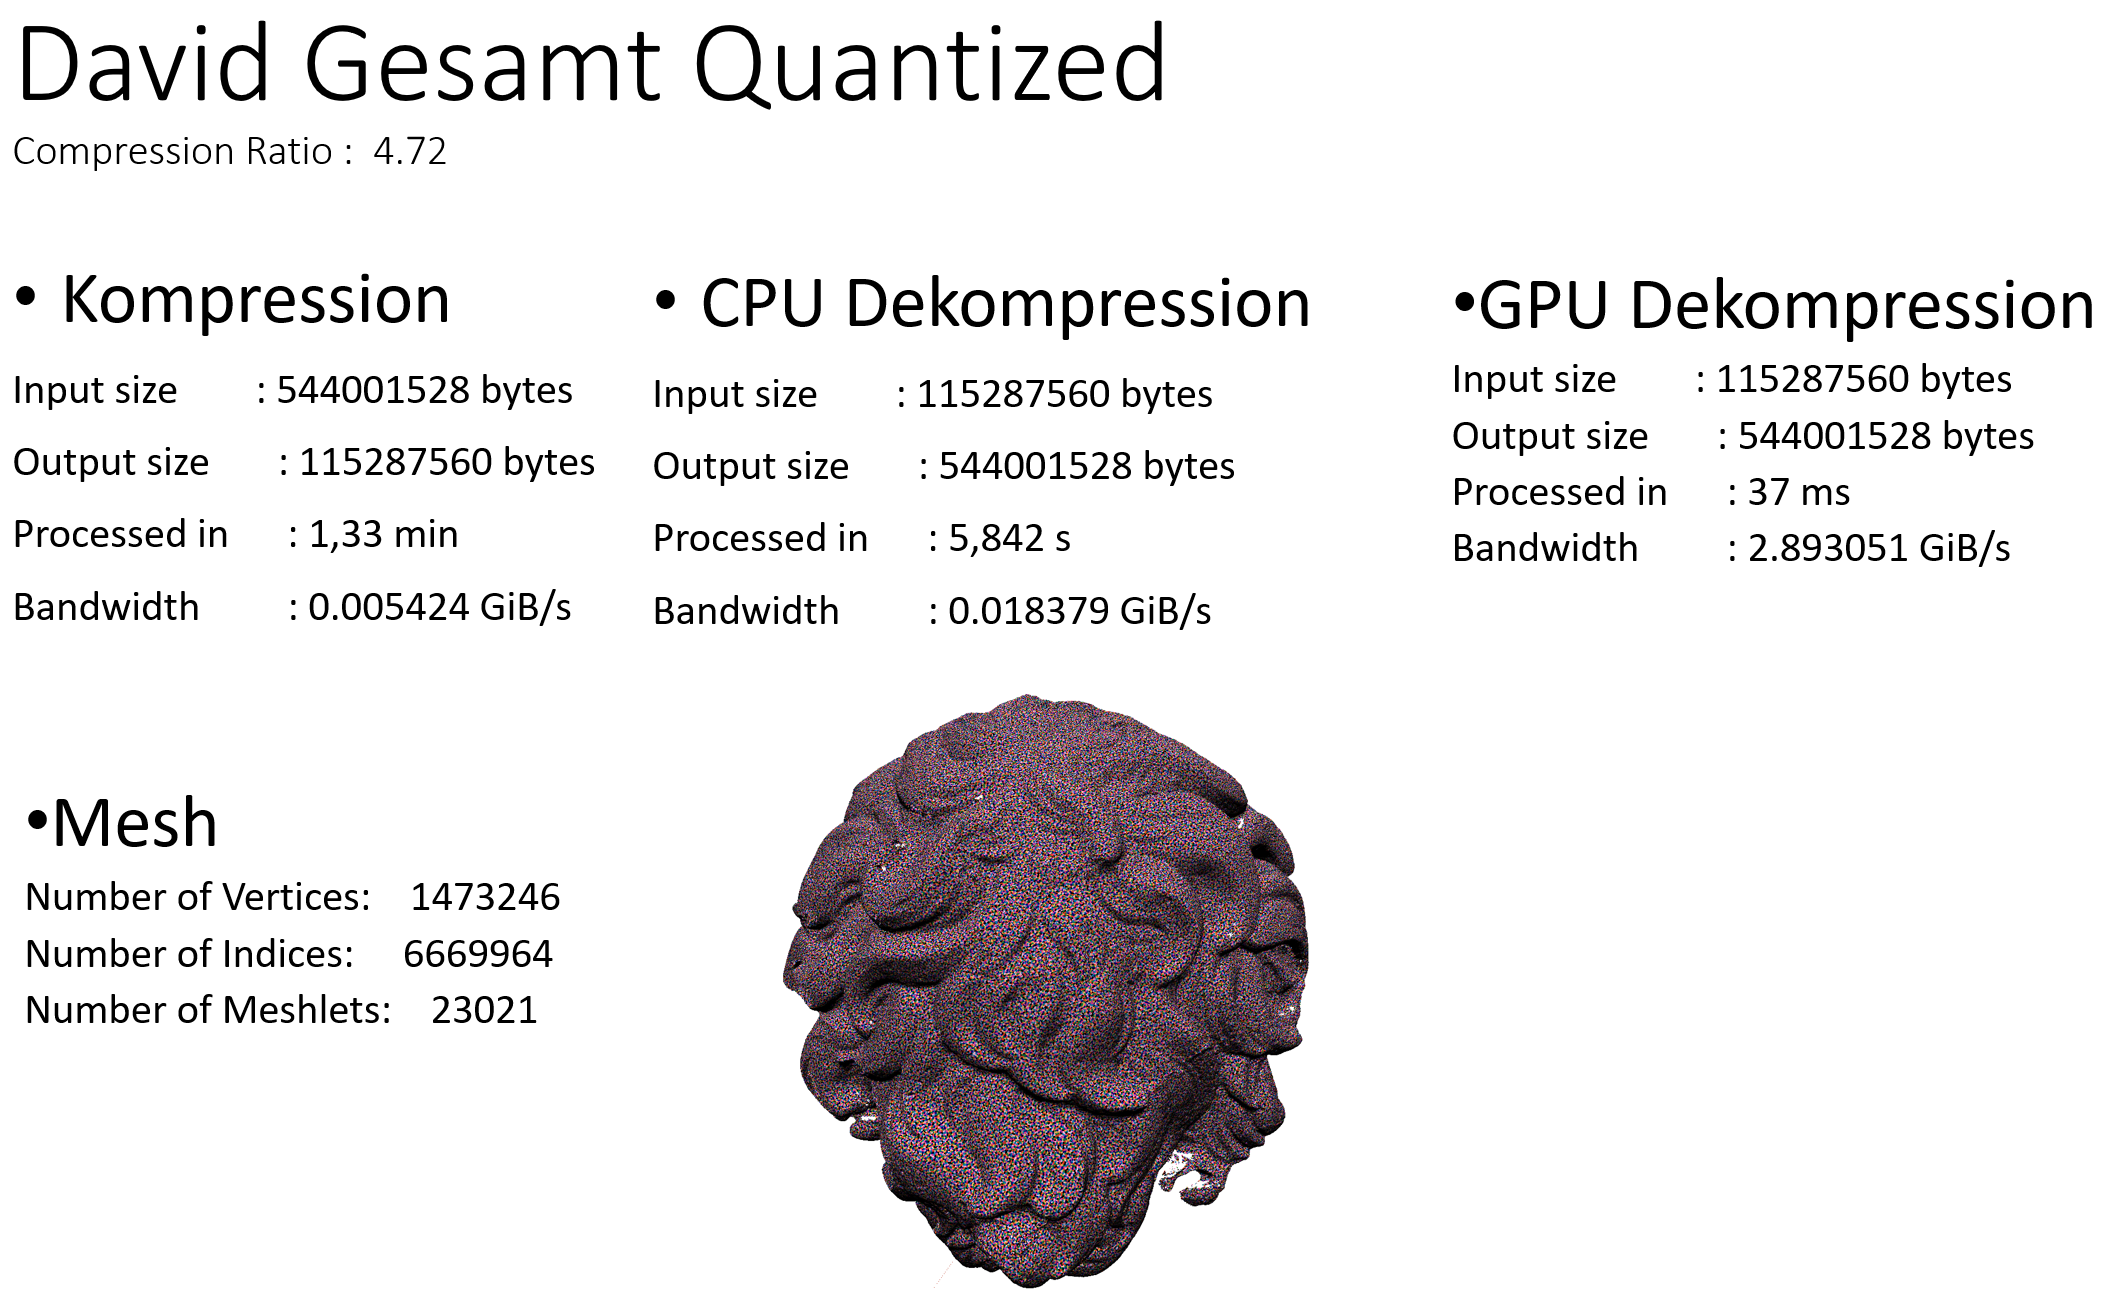
\includegraphics[scale=0.28]{Bilder/ergebnisse_full/david_quantized.png}
\end{figure}
\clearpage
\subsection{Berechnung der verwendeten Prozentzahlen}
\begin{figure}[h]
  \centering  
  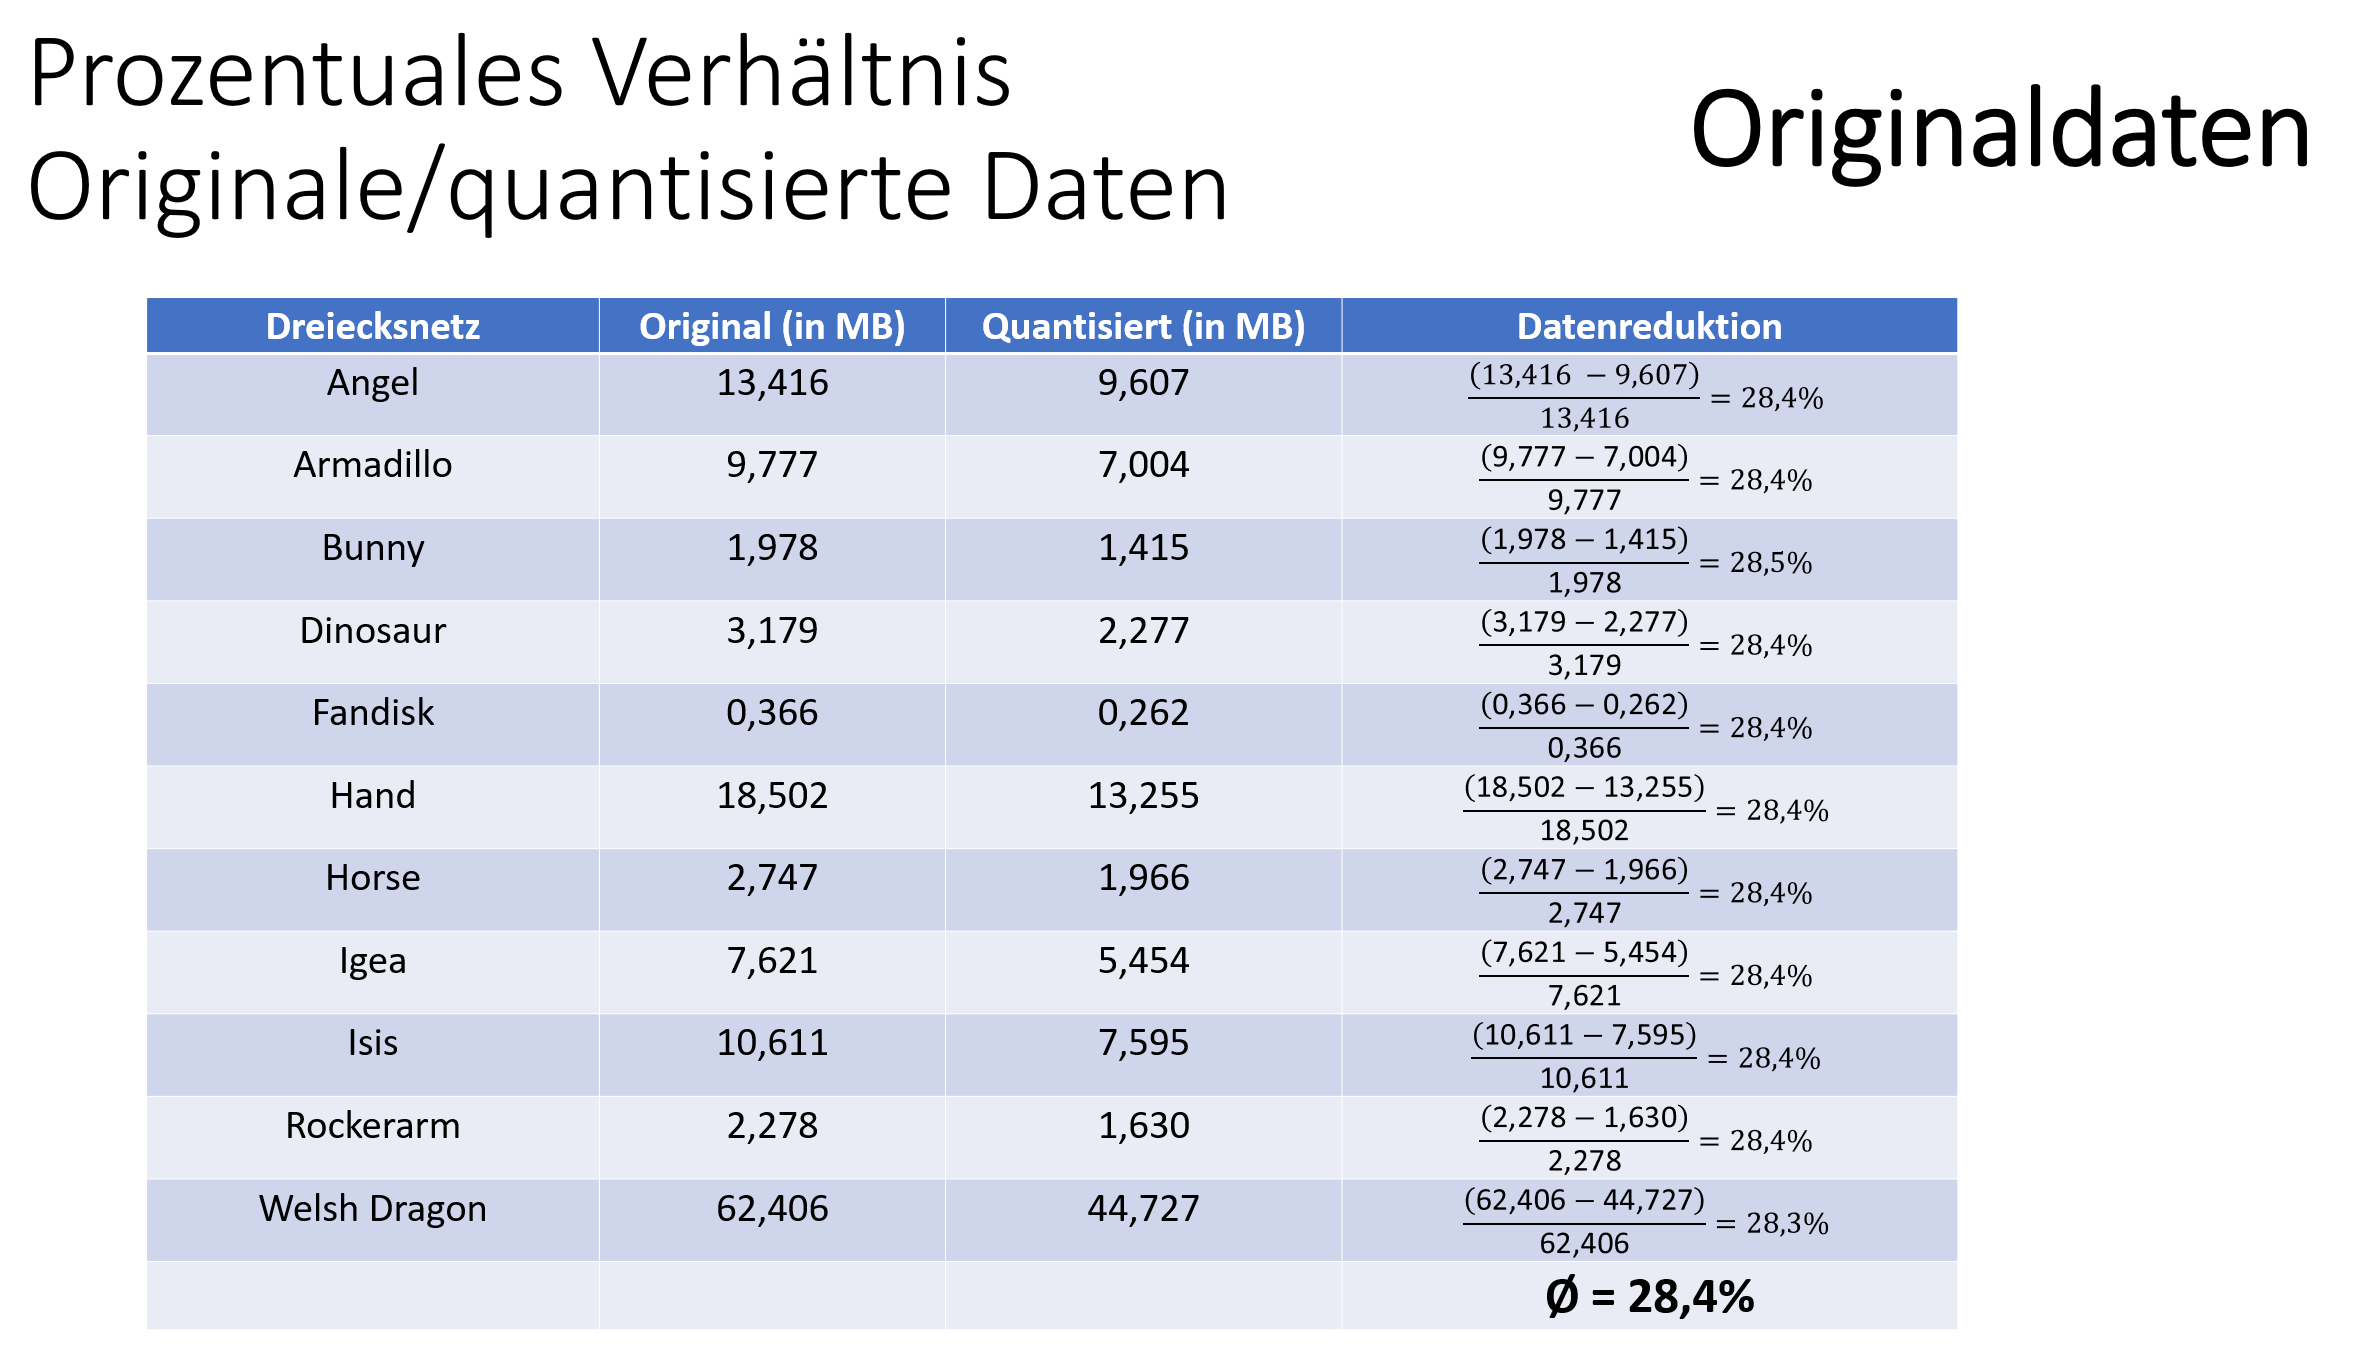
\includegraphics[scale=0.24]{Bilder/ergebnisse_full/orig_proz.png}
\end{figure}
\begin{figure}[h]
  \centering  
  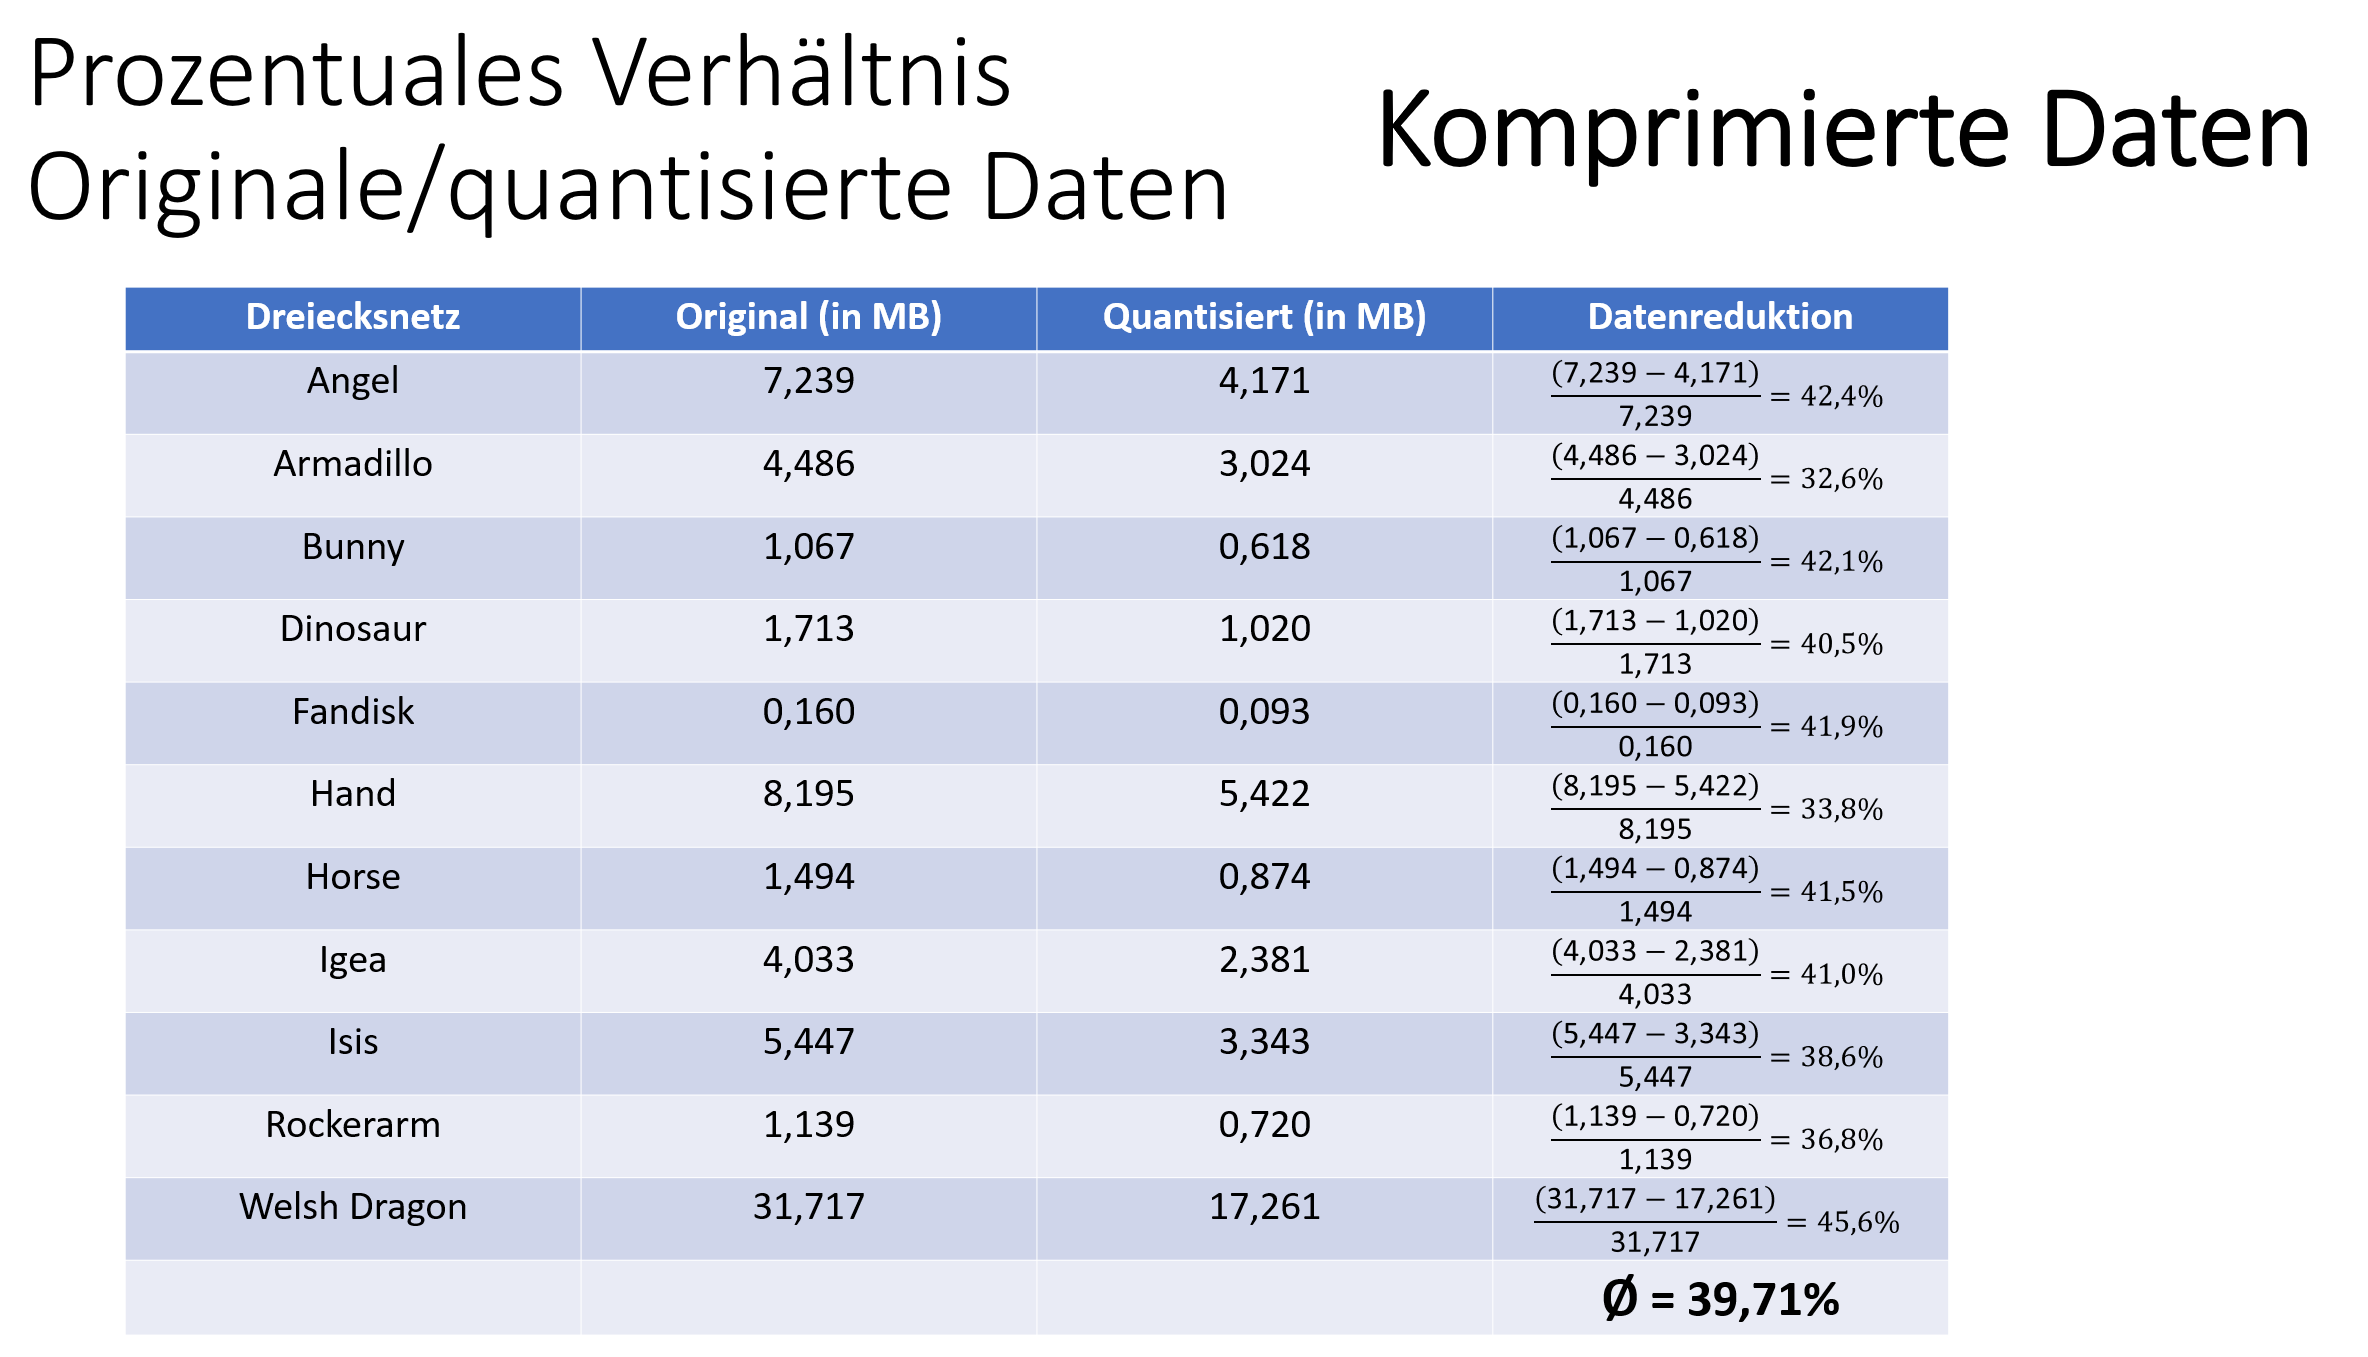
\includegraphics[scale=0.24]{Bilder/ergebnisse_full/komp_proz.png}
\end{figure}
  }{}

  % Declaration of Honor
  \newpage
  \phantomsection
  \addcontentsline{toc}{section}{Ehrenwörtliche Erklärung}
  \lhead{Ehrenwörtliche Erklärung}
  \pagestyle{plain}
\pagenumbering{gobble}


\textbf{{\Large Ehrenwörtliche Erklärung}}
\vspace{2cm}

% Determine article for document type
\ifthenelse{\equal{\DocumentType}{Praxisbericht}}
  {\newcommand{\DocumentArticle}{meinen}}
  {
    \ifthenelse{\equal{\DocumentType}{Bachelorarbeit}}
      {\newcommand{\DocumentArticle}{meine}}
      {
        \ifthenelse{\equal{\DocumentType}{Masterarbeit}}
          {\newcommand{\DocumentArticle}{meine}}
          {\newcommand{\DocumentArticle}{meine/n}}
      }
  }

Ich versichere hiermit, dass ich \DocumentArticle\ \DocumentType \ mit dem Titel
\vspace{1cm}

\begin{tabular*}{\linewidth}{@{\extracolsep{\fill}}ccc}
 \\ \hline
 \vspace{2cm}
 \\ \hline
\end{tabular*}
\vspace{2cm}

selbständig verfasst, keine anderen als die angegebenen Quellen und Hilfsmittel benutzt
sowie nicht an anderer Stelle als Prüfungsarbeit vorgelegt habe.
\vfill

\begin{table*}[hp]
  \centering
  \begin{tabular}{L{6cm}L{2cm}L{6cm}}
    & & \\
    & & \\ \cline{1-1}
    Ort &  \\
    & & \\
    & & \\
    & & \\
    & &  \\ \cline{1-1} \cline{3-3}
    Datum & & Unterschrift \\
  \end{tabular}
\end{table*}

  % TODO list
  \iftotalcounttodos
    \listoftodos[TODOs]
  \fi

  \end{document}
}

% ===========================================================================
%                   Simplified centered & colored tables
% ===========================================================================

\newenvironment{colortable}[1]{
  \begin{center}
    \begin{tabular}{#1}
    \hline
    \rowcolor{Gray}
}
{
    \hline
    \end{tabular}
  \end{center}
}

\newcommand{\tablecontent}{
  \hline
  \rowcolor{White}
}


\def\Studiengang{Informatik}
\def\Autorenname{Janek Foote}
\def\Dozent{Quirin Meyer}
\def\Titel{Geometriedekompression von Dreiecksnetzen auf der GPU}

% Infos zum Unternehmen
\def\Unternehmen{<FIRMENNAME>}
\def\Abteilung{<ABTEILUNG>}
\def\Strasse{<STRAßE>}
\def\Ort{<ORT>}

% Infos zum Betreuer
\def\Betreuer{Quirin Meyer}
\def\Funktion{<FUNKTION BETREUER>}
\def\Telefon{<TELEFONNUMMER BETREUER>}
\def\Email{<BETREUER EMAIL>}

% Daten
\def\Beginn{<BEGINN>}
\def\Ende{<ENDE>}
\def\Abgabe{12.04.2024}

\startHSCdocument[Bachelorarbeit]

  \section{Einführung}

In der Computergrafik ist die Erzeugung eines Dreiecksnetzes eine gängige Methode zur Generierung von 3D-Modellen. Diese Modelle können in Topologie und Geometrie unterteilt werden. Für die Geometrie werden verschiedene Attribute benötigt. 
So werden die Positionen, die Normalenvektoren und Texturekoordinaten/Farbwerte für jeden Punkt des Dreiecksnetzes in single-precision floating point values (32 Bit Gleitkommazahlen) gespeichert. 
Für die korrekte Annordung und Reihenfolge der Knotenpunkte ist die Topologie zuständig. 
Dabei ist die Datenkompression ein entscheidendes Thema. 
In einer Welt, in der digitale Daten schon lange ein wichtiges Thema sind, und dennoch immer weiter an Bedeutung gewinnen, ist die effiziente Speicherung und Übertragung ein wichtiger Gesichtspunkt.
3D Modelle werden so gut wie überall benötigt. 
Videospiele und Animationsserien wären ohne nicht vorstellbar. 
Architekten können ihre Ideen auch ohne Bleistift auf das Papier (oder den Bildschirm) bringen.
Künstler wollen Modelle erschaffen, die den Eindruck gewinnen wollen, realitätsgetreu zu sein. 
Die Folge davon ist, dass diese Modelle stetig komplexer werden, und somit ein größerer Speicheraufwand benötigt wird. 
Um dem entgegenzuwirken, werden Methoden verwendet, diese digitalen Informationen zu komprimieren. \newline

\subsection{Geschichtliche Ausarbeitung Thema Datenkompression}
\label{subsec:main_kompression}
Ursprünglich zur Repräsentation von Daten entwickelt, wurde der Morse Code zu einem der wichtigsten Werkzeuge für die Kommunikation des 19. Jahrhunderts. 
Bestehend aus zwei Grundbausteinen, einem kurzen und einem langen Signal, konnten einzelne Buchstaben kodiert werden. 
Erweitert man dieses Alphabet mit einem weiteren \glqq Symbol\grqq\, einer Pause, die zwischen einzelnen Signalsequenzen eingelegt wird, können ganze Sätze übermittelt werden. 
Das bekannteste Werkzeug für den Morse Code ist der Telegraf, mit dem diese Signale über weite Strecken übertragen werden konnten.
Die Erfindung des Morsecodes findet im 21. Jahrhundert nicht nur seinen Zweck in dramatischen Momenten des in Film und Fernsehens. 
Es war zeitgleich ein früher und großer Meilenstein und Wegbegleiter für die Kompression einer Datenquelle (in diesem Fall das Alphabet). 
Durch Untersuchungen einer großen Anzahl an Literatur kann eine Buchstabenhäufigkeit berechnet werden. 
Diese sagt aus, wie wahrscheinlich es ist, welcher Buchstabe in einem Text folgt, ohne den aktuellen Kontext, in Form von vorgehenden Buchstaben, zu betrachten.
Da die Wahrscheinlichkeit eines Zeichens abhängig vom Alphabet ist, sollten diese nicht übergreifend verwendet werden. 
So sind die Buchstaben \glqq E\grqq\ und \glqq T\grqq\ die Buchstaben des englischen Alphabets, welche die höchste Auftrittswahrscheinlichkeit besitzen, während sich im deutschen Alphabet der Buchstabe \glqq E\grqq\ von der Masse abhebt.
%Datenkompression problem ausführen: durch ein stop Signal geht eine wichtige Eigenschaft verloren (eventuell binär)
Der Morse Code hat gezeigt, welchen Nutzen die Kompression von Information beinhaltet.
Zu Kriegszeiten hat dieser eine effiziente und schnelle Übermittlung von Informationen ermöglicht.
Dadurch konnte in Krisenmomenten schnell reagiert werden, um so größeren Katastrophen frühzeitig abzuwenden, aber leider auch zu verursachen.

\subsubsection*{Der Ist-Stand}
Springen wir in die heutige Zeit sehen wir die Auswirkung von komprimierten Daten.
Die meisten Menschen denken an JPEGs und PNGs, wenn sie an digitale Bilder denken.
Bekanntere Videoformate sind MP4, AVI und FLV.
Bei all diesen Formaten handelt es sich um komprimierte Rohdaten.
Das Filesystem eines jeden relevanten Betriebssystems komprimiert beim Speichern von Daten diese automatisch.
Zusätzlich dazu besteht noch die Möglichkeit, seine Daten manuell zu komprimieren mithilfe von Programmen wie 7Zip, WinRar oder WinZip.
Datenkompression kann in so gut wie allen Bereichen angetroffen werden.
Und die Gründe dafür sind simpel.
Speicherplatz ist teuer, und das Ressourcenmanagement wird deutlich vereinfacht, wenn die benötigte Hardware minimiert wird.
Betrachten wir das Streamen von Daten auf dem Beispiel des größten Videostreaming Dienstes Youtube.
Laut Statistiken werden pro Minute hunderte Stunden an Videomaterial hochgeladen Tendenz steigend (Abb.~).
\begin{figure}[htb]
  \centering  
  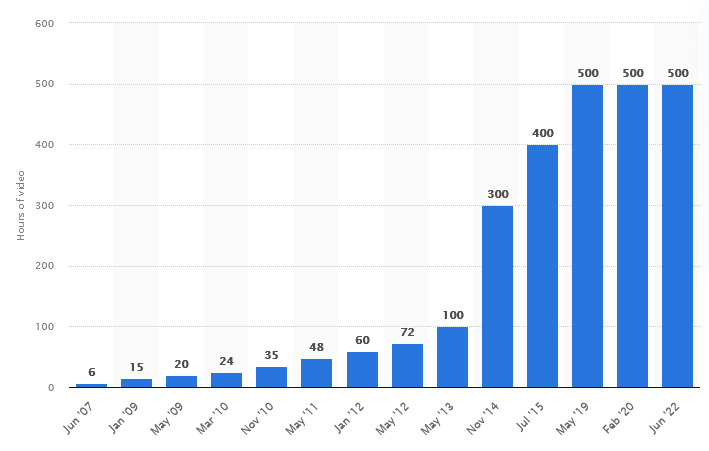
\includegraphics[scale=0.8]{Bilder/youtube_statistik.png}
  \caption[Youtube Statistik]{\textbf{Anzahl der Youtube Videos} Die Anzahl an Minuten die auf Youtube hochgeladen werden.
  Abbildung von Statista: https://www.statista.com/statistics/259477/hours-of-video-uploaded-to-youtube-every-minute/ }
  \label{fig:youtube}
\end{figure}
Um die Unmengen an Videos zu speichern, benötigt Google riesige Serverfarmen, die auf dem gesamten Globus verstreut sind.
Eine genaue Zahl ist der Öffentlichkeit nicht bekannt, es steht jedoch außer Frage, dass diese nochmal um einiges höher ausfällt, würde es keine Verfahren zur Datenkompression geben. \newline

Ein weiterer Gesichtspunkt ist der eigentliche Nutzen von Youtube, dem Streamen von Videos.
Um ein Video sehen zu können, muss dieses von dem Youtube Server, zum Nutzer, dem Client übertragen werden.
Durch die Komprimierung der Quelldateien sind die zu übertragenden Daten schon geschrumpft.
Es können jedoch noch weitere Schritte absolviert werden, um die Daten für den Nutzer besser zugänglich zu machen.
Dazu werden Verfahren wie Trancoding, Transsizing und Transrating verwendet.
Transcoding beschreibt den Prozess, ein bereits komprimiertes Videoformat in ein anderes, eventuell für den Client besser zugeschnittenes Videoformat zu komprimieren.
Das sollte jedoch nicht zu oft angewendet werden, da die Qualität beim wiederholten dekomprimieren und komprimieren verloren geht, sollten die Verfahren verlustbehaftet sein. \newline
In vielen Fällen kann die originale Auflösung vom Endgerät nicht abgespielt werden, und wird deshalb von diesem auf eine niedrigere Auflösung skaliert.
Beispielsweise wenn das Endgerät lediglich 1080p auflösen kann, aber ein Video in 4K Auflösung gestreamt werden soll.
Trotzdem werden die vollen Daten des Videoformats empfangen.
Um diese Verschwendung von Bandbreite zu sparen, wird Transsizing verwendet.
Die originalen Daten werden in eine kleinere Auflösung skaliert, und anschließend übertragen. \newline
Um die Bitrate zu minimieren wird Transrating verwendet.
So kann die Auflösung beibehalten werden bei jedoch geringere Bitrate.
Die Verfahren zur Minimierung des Datenstroms hören sich zunächst sehr mächtig an, sind jedoch mit Vorsicht zu genießen.
Der Vorgang ist nämlich Verlustbehaftet und kann bei zu starker Nutzung zu Artefakten führen.
Dafür ermöglicht es jedoch Menschen, deren Internetzugang ein Abspielen in hoher Qualität nicht zulässt, den Streaming Anbieter zu nutzen.

Der Ursprung der Datenkompression ist dementsprechend der Weiterentwicklung des Morse Codes zurückzuführen. 

TODO

\subsection{Steigende Komplexität}
\label{subsec:steigende_komplexität}
Um die Realität bestmöglich darzustellen, werden Modelle stetig detailreicher, wodurch die Anforderungen an der Hardware steigen. In einer komplexen Szene können mehrere Millionen Dreiecke sichtbar sein, die je nach Anwendung, in Echtzeit gerendert werden müssen. Der Wunsch nach realistischeren Modellen in der Animationsfilm und Videospielbranche hat die Dreiecksanzahl von 3D Modellen in die Höhe schießen lassen. 

\subsection{Ziel der Arbeit}

  \section{Grundlagen}

Obwohl Dreiecksnetze eine effektive Darstellung bieten, 3D-Modelle darzustellen, beanspruchen diese sehr viel Speicherplatz.
Mithilfe von Brotli-G sollen diese auf der CPU komprimiert, und auf der GPU dekomprimiert werden, sodass diese fertig zur Darstellung sind, ohne viel Bandbreite zu nutzen.
Damit der Weg von Komprimierung zu Darstellung verständlich ist, müssen einige grundlegende Dinge geklärt werden.

In diesem Grundlagenkapitel werden die von Brotli-G genutzen Algorithmen erläutert.
Zusätzlich wird ein Ausblick auf die Grafikpipeline gegeben, und die Stellen betrachtet, bei denen weitere Verbesserungen vorgenommen werden können.
Diese zeigt alle Transformationen, die die Daten eines Dreiecksnetzes von dem GPU Buffer bis zum Bildschirm durchläuft.

\subsection{Brotli Kompressionsstandard}
\label{subsec:brotli}
Brotli-G ist eine Weiterentwicklung des Brotli Kompressionsstand, der von AMD im Jahre 2022 entwickelt und veröffentlicht wurde.
Die AMD Spezifikation bietet parallele Datenverarbeiten nach dem SIMD Prinzip (Kap.~\ref{fig:simd_pattern}) auf Parallelrechnern, wie GPUs und Multithreaded CPUs.
Zum Verständnis des von AMD veröffentlichten Kompressionsmodells ist zunächst ein Blick auf das Original erforderlich. \newline

Brotli ist ein von Google Research entwickelter Kompressionsstandard, der 2013 veröffentlicht wurde.
Er ist darauf ausgelegt, Webinhalte effizienter zu komprimieren als ältere Standards wie Gzip oder Deflate.
BrotliG wurde mit bedacht auf Kompatibilität mit dem offiziellen Brotli entwickelt.
So sollte Brotli auch in der Lage sein, Inhalte, die mit BrotliG komprimiert wurden, zu entschlüsseln.
Zu beachten ist, dass dies nur in diese Richtung funktioniert, und somit Brotli das BrotliG Format nicht dekodieren kann  \cite{BrotliG2022}.

Brotli verwendet eine Kombination vieler Kompressionsalgorithmen, um Inhalte effizient zu komprimieren. 
Brotli's Kern besteht aus einem LZ77 Algorithmus, der in unterschiedlichen Ausführung auch in anderen Kompressionsstandard verwendet wird.
Der LZ77 Algorithmus wird zusätzlich mittels Huffman Codierung optimiert.

\subsection{Parallele Datenverarbeitung}
\label{subsec:flynn}
Michael Flynn unterteilte Rechnerarchitekturen in Kategorien, die Abhängig von der Anzahl der Instruktions- und Datenströme sind. \newline
Die Instruktions- und Datenströme:
\begin{enumerate}
\item[\textit{SI}] (\textbf{S}ingle \textbf{I}nstruction)
\item[\textit{MI}] (\textbf{M}ultiple \textbf{I}nstruction) 
\item[\textit{SD}] (\textbf{S}ingle \textbf{D}ata) 
\item[\textit{MD}] (\textbf{M}ultiple \textbf{D}ata) 
\end{enumerate}
können kombiniert werden. \newline

Dadurch ergeben sich die vier Rechnerarchitekturen \textit{SISD}, \textit{SIMD}, \textit{MISD}, \textit{MIMD}.
\subsubsection*{SISD (Single Instruction, Single Data)}
Die am häufigsten anzutreffene Rechnerarchitektur.
Bekannter unter den Namen Von-Neumann Architektur bearbeitet diese Architektur die auf dem Speicher befindlichen Daten seriell.
Man redet auch von skalaren Operationen auf die Daten.
Rechnerarchitekturen mit SISD sind leicht zu verstehen und die Verarbeitung ist vorhersehbar.
Der Preis dafür ist jedoch die langsame Geschwindigkeit gegenüber parallelen Architekturen.
\subsubsection*{SIMD (Single Instruction, Multiple Data)}
Um die Geschwindigkeit zu erhöhen, werden Daten, auf denen die selbe Operation ausgeübt wird, parallel verarbeitet.
Das ist bei der Berechnung von Vektoren und Matrizen von Vorteil.
Betrachten wir die Addition zweier Vektoren, so kann der resultierende Vektor berechnet werden, wenn die einzelnen Komponenten der Vektoren addiert werden (siehe Abb.~\ref{fig:simd_pattern}). Der Vertex Shader macht von dieser diesem Konzept Gebrauch, während dieser seine per-Vertex Operationen ausführt \cite{DalCin1996}.
\begin{figure}[htb]
  \centering  
  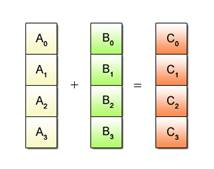
\includegraphics[scale=1.0]{Bilder/Simd_pattern.jpg}
  \caption[SIMD Pattern]{\textbf{Parallele Addition von Daten} In der Abbildung ist eine Addition verschiedener Daten zu sehen. Da die selbe Operation ausgeübt wird können die einzelnen Komponenten parallel verarbeitet werden.
  Abbildung ist aus http://ftp.cvut.cz/kernel/people/geoff/cell/ps3-linux-docs/CellProgrammingTutorial/BasicsOfSIMDProgramming.html }
  \label{fig:simd_pattern}
\end{figure} 
\subsubsection*{MISD (Multiple Instruction, Single Data)}
Um alle Kombinationen von Daten und Instruktionsströmen zu zeigen wurde auch MISD definiert.
Die Rechnerarchitektur bezieht sich darauf, das auf nur einem Datenpunkt verschiedene Operationen ausgeführt werden.
Für eine lange Zeit war diese Art von Rechnerarchitektur rein theoretisch anzutreffen, da weder 
\subsubsection*{MIMD (Multiple Instruction, Multiple Data)}
Wie auch die SIMD Architektur ist MIMD in Parallelrechnern anzutreffen.
Das Operationsprinzip von MIMD ist die Datenparallelität.
Das Funktionsprinzip von MIMD-Rechnern umfasst die gleichzeitige Ausführung von Anweisungen durch mehrere Prozessoren, die entweder über gemeinsame Variablen oder durch Nachrichten miteinander kommunizieren \cite{DalCin1996}.
TODO später \cite{Jakob2017} \newpage

\subsection{Die traditionelle Rendering Pipeline}
\label{subsec:traditionelle_renderingpipeline}
Um den Nutzen der neu vorgestellten Task- und Mesh-Shader Pipeline zu verstehen, muss zunächst die traditionelle Pipeline dort betrachtet werden, wo sie verbessert werden kann.
Die Rendering Pipeline besteht aus eine Reihe von programmierbaren (Abb.~\ref{fig:traditional_pipeline} grün dargestellt) und fixed-function (Abb.~\ref{fig:traditional_pipeline} türkis dargestellt) Stages.
Dazu kommt, das einige dieser Stages optional sind.
\begin{figure}[htb]
  \centering  
  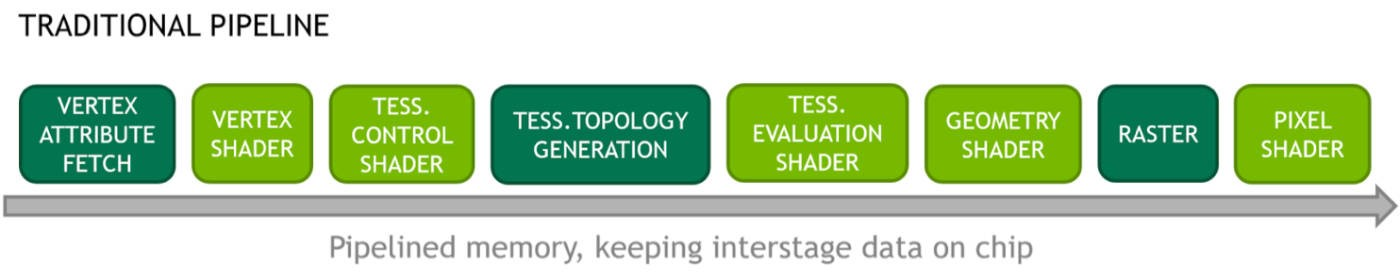
\includegraphics[scale=0.43]{Bilder/traditionelle_pipeline.jpg}
  \caption[traditionelle Rendering Pipeline]{\textbf{traditionelle Rendering Pipeline} \newline Die Abbildung beschreibt den Verlauf durch die einzelnen Shader Stages, die jeder Vertex macht. Entnommen wurde diese aus dem NVidia Blogpost \cite{Kubisch2018}}
  \label{fig:traditional_pipeline}
\end{figure}
\newline
Im GPU Memory angekommen, liest die \textit{Vertex Attribute Fetch} Stage die Vertex Daten aus, und sendet diese an den Vertex Shader.
Die Vertex Daten werden dort in die benötigten Koordinatensysteme transformiert und der optionalen Tessellation Stage weitergegeben, falls diese verwendet wird.
Die Tessellation Stage ist dazu da, Patches von Primitiven in kleinere Primitiven zu unterteilen.
Der optionale Geometry Shader kann dazu verwendet werden, weitere Vertices zu generieren.
Im Rasterizer angekommen, werden Primitiven verarbeitet und daraus Fragmente berechnet, denen der Fragment Shader zum Abschluss ihre Farbe gibt. \newline
Im Folgenden werden die einzelnen Stages nochmal genauer erläutert.

\subsubsection{Vertex Shader}
\label{subsubsec:vertex}
Zunächst wird der vom Entwickler programmierbare Vertex Shader angesteuert.
Dieser ist nicht optional, da alles nachfolgende auf den ausgegebenen Vertices aufbaut.
Hier können Operationen auf einzelnen Vertices ausgeführt werden.
Dafür wird der Vertex Shader für jeden Vertex einzeln aufgerufen.
Hier zeichnet sich das SIMD Modell der GPU aus (Kap~\ref{subsec:flynn}), da der Vertex Shader von mehreren Prozessoren auf unterschiedlichen Vertices zeitgleich operiert.
Die Inputs des Vertex Shaders werden mittels \textit{Vertex Attribute Locations} in den Shader eingebunden.
Der Shader kann dadurch die Positionen, Normalen und Texturkoordinaten von der CPU aufnehmen.
Eine Einschränkung, die dabei aufkommt, ist das Verhältnis von Eingabe und Ausgabe Vertices.
Der Shader erwartet, dass für jeden Eingabe Vertex auch ein Vertex ausgegeben wird.
Die Vertex Position wird für gewöhnlich in den Clip-Space transformiert, und der Pipeline weitergegeben.

\subsubsection{Tessellation Stage}
\label{subsubsec:tesselation}
Die Ausgabe Vertices des Vertex Shaders gelangen anschließend in die optionale Tessellation Stage.
Der generelle use-case ist, einen Patch an Primitiven in wiederum kleinere Primitiven zu verarbeiten. 
Die Tessellation Stage wird in drei Schritte unterteilt.
Darunter ist mit dem \textit{Tessellation Control Shader} (TCS) ein optional programmierbarer Schritt, eine fixed-function mit der \textit{Primitive Generation} und einen programmierbaren \textit{Tessellation Evaluation Shader} (TES).

\subsubsection*{Tessellation Control Shader (TCS)}
Der \textit{Tessellation Control Shader (TCS)} (der wiederum optional ist), ist ein geeigneter Schritt um das \textit{LOD} (Level of Detail) zu berechnen und unter gewissen Voraussetzungen vorab einige Patches zu cullen. 
Ein Patch beschreibt eine Anzahl an Primitiven.
Aus der Subdivision dieses Patches werden weitere Vertices berechnet, die zur Verarbeitung in den nächsten Schritt der Pipeline geschickt werden.
Im TCS wird der Grad der Tessellation, das Spacing zwischen subdivided Punkten und die gewünschte Topologie festgelegt.
Genauer gesagt wird hier gesetzt, wie oft die Primitiven unterteilt werden und welche Form diese am Ende haben sollen (triangle, quad, isolines).

\subsubsection*{Tessellation Topology Generation (TPG)}
Mit der fixed-function stage des Tessellation Schritts werden die Primitiven mittels den im TCS bestimmten Parametern unterteilt.
Die Koordinaten werden anschließend für den Tessellation Evaluation Shader berechnet.
Diese unterteilt die Patches abhängig von den Berechnungen der TCS.

\subsubsection*{Tessellation Evaluation Shader (TES)}
Der \textit{Tessellation Evaluation Shader} hat den einfachsten Job und realisiert lediglich die Arbeit, die von den zwei vorherigen Stages verrichtet wurde.
Die berechneten Koordinaten des TPG werden in dieser Shader Stage interpoliert, um die neuen Vertices zu generieren.
Abschließend werden die aus der Subdivision berechneten Vertices ausgegeben. 
Wenn der optionale TCS nicht genutzt wird, werden default Parameter für den TPG benutzt. \cite{cozzi2012opengl}\cite{Carvalho2022}

\subsubsection{Geometry Shader}
\label{subsubsec:geometry_shader}
Ein weiterer optionaler Schritt in der traditionellen Grafikpipeline ist der \textit{Geometry Shader}.
Er bekommt eine Primitive als Input, und kann keine oder auch mehr Primitiven ausgeben, als er bekommen hat.
Die Fähigkeit zusätzliche Vertices zu generieren ist auch das, was den Geometry Shader besonders macht.
Der Geometry Shader bekommt seinen Input entweder vom TES, oder, wenn die Tessellation Stage keine Verwendung findet, vom Vertex Shader und leitet seine Ausgabe an den Fragment Shader weiter.
Um Bandbreite zwischen CPU und GPU zu sparen, kann ein Geometry Shader ein Dreiecksnetz mit wenigen Dreiecken erweitern und dieses so detaillierter gestalten.
Ähnlich wie bei der Tessellation, die auf \textit{Patches} von Primitiven agiert, verarbeitet der Geometry Shader die Primitiven an sich.

\subsubsection{Pixel Shader}
\label{subsubsec:pixel_shader}
Der Pixel bzw. Fragment Shader ist der letzte programmierbare Schritt der Grafikpipeline.
In diesem werden die transformierten Vertices und Primitiven schlussendlich gezeichnet.
Der Pixel Shader operiert jedoch nicht auf diesen Daten, sondern auf sogenannten \textit{Fragmenten}.
Das bedeutet, bevor der Pixel Shader seinen Input bekommt, müssen Vertices und Primitiven erst durch den Rasterizer.
Nun liegt es am Entwickler, den einzelnen Fragmenten ihre Farbe zu geben.
In einem Modell werden per-Vertex Texturkoordinaten gesetzt, die auf eine Texturemap verweisen.
Im Fragment Shader wird diese Texturemap mittels Sampler interpoliert.
Zusätzlich müssen noch Materialeigenschaften beachtet werden.
Alternativ kann jeder Vertex auch seinen eigenen Farbwert besitzen. \newline

Um der Szene mehr Realismus beizusteuern, kann im Fragment Shader auch ein Lichtmodell implementiert werden.
Beispiele dafür sind \textit{Flat shading}, \textit{Gouraud shading} und \textit{Phong shading}.
Für die Lichtberechnung werden die Oberflächen-Normalen benötigt.
Diese sind entweder in einem Dreiecksnetz gegeben, oder müssen noch berechnet werden.
Ausgabe des Pixel Shaders ist wiederum ein Fragment.

\subsection{Compute Shader}
\label{subsec:compute_shader}
Der Compute Shader gehört nicht zur traditionellen Grafikpipeline, kann darin aber seinen Nutzen finden.
Sie dienen dazu, jede Mögliche Information die gewünscht ist auf der GPU zu berechnen.
Anders als bei den Shader Stages der traditionellen Grafikpipeline (Kap.~\ref{fig:traditional_pipeline}), erwartet der Compute Shader keine definierten Input/Output Daten, wie beispielsweise der Vertex Shader, der als Input und Output einen Vertex erwartet.
Der Compute Shader kann also willkürliche Daten verarbeiten und dabei noch die Parallelisierung der GPU nutzen \cite{Compute24}. \newline

Wie schon gesagt erhält der Compute Shader keine Input Variablen wie beispielsweise der Vertex Shader.
Im Gegensatz zu diesem werden benötigte Daten mittels Buffer und \glqq Shader Ressource Views\grqq\ auf die GPU geladen (in D3D12).
Aber ganz ohne Inputs kommt der Compute Shader nicht aus.
Vor Aufruf des Compute Shaders muss bestimmt werden, mit wie vielen Threads dieser arbeiten soll.
Der Aufruf der Dispatch Methode mittel Grafik API führt dazu, das der aktuell aktive Compute Shader aufgerufen wird.
Die Dispatch Methode nimmt die Anzahl an Threads in drei Dimensionen als Argument.

Dafür gelten jedoch Hardware Limitierungen.
Für die Anzahl der Threads muss gelten
\begin{gather*}
	numThreadsX, numThreads, numThreadsZ \leq 128 \\
	numThreadsX * numThreadsY * numThreadsZ = 1024
\end{gather*}
(Für Compute Shader Version 5\_0)

Um das SIMD Konzept des Compute Shaders zu verstehen sind zwei Variablen elementar wichtig.
SVGroupThreadID und SVGroupID.
TODO

\subsection{Grundbegriffe der Datenkompression}
\label{subsec:grundbegriffe_datenkompression}

Entscheidungsgehalt
Redundanz
Entropie

  \section{Methodik}
\label{sec:methodik}

Die vorliegende Bachelorarbeit beschäftigt sich mit der Dekodierung verschiedener Dreiecksnetze mittels dem Kodierungstandard Brotli-G.
Diese Methodiksektion dient dazu, einen detaillierten Einblick auf die Durchführung und Analyse des Experiments zu geben.
Das Experiment zielt darauf ab, komprimierte Dreiecksnetze auf der GPU zu dekomprimieren.
Insbesondere sollen das Kompressionsverhältnis, Dekompressionsgeschwindigkeit und die visuelle Qualität quantitativ ausgewertet werden.

\subsection{Ablauf des Experiments}
\label{subsec:ablauf}
In diesem Abschnitt folgt eine kleine Beschreibung, wie die Kompressionspipeline aussieht.
In den Folgenden Kapiteln werden die einzelnen Teilschritte genauer erläutert. \newline
Zu Beginn muss der Datensatz mittels Brotli-G kodiert werden.
Der Einfachheit halber wird in diesem Abschnitt von einem einzigen Dreiecksnetz gesprochen.
Der Meshoptimizer von Zeux \cite{Zeux} ist dafür verantwortlich, aus den Positionen und Indizes die Meshletdaten zu generieren.
Dazu wurde ein Binärformat entworfen, welches die relevanten Daten zum Darstellen des gesamten Dreiecksnetzes speichert.
Das Binärformat besteht dementsprechend aus dem Meshlet Descriptor, Vertex Ressourcen (Positionen und Normalen) und den Indizes zur Primitivengenerierung. \newline
Dieses Binärformat wird als gesamtes komprimiert.
Anschließend werden die GPU Resourcen für die Eingabe (komprimiertes Dreiecksnetz) und Ausgabe (dekomprimiertes Dreiecksnetz) angelegt. \newline
Für die Ausgabe wird eine \glqq Unordered Acces View (UAV)\grqq\ verwendet.
Wie der Name schon vermuten lässt, bietet diese eine flexiblere Möglichkeit, gleichzeitig an verschiedenen Orten zu lesen und schreiben.
Besonders von Vorteil ist dieser Ressourcentyp für die parallele Verarbeitung.
So können einzelne Threads von der Ressource lesen/schreiben, ohne warten zu müssen, bis ein anderer Thread die Ressource wieder freigibt \cite{Microsoft2021}. \newline
Die UAV wird im Compute Shader als Output Buffer gesetzt, und mit den dekomprimierten Daten des Dreiecksnetzes gefüllt.

Abschließend wird die UAV im Mesh Shader gesetzt und die Meshlets und somit das gesamte Dreiecksnetz werden aus den Binärdaten rekonstruiert. \newline
Der gesamte Vorgang ist in Abbildung~\ref{fig:projekt} zu sehen.

\begin{figure}[htb]
  \centering  
  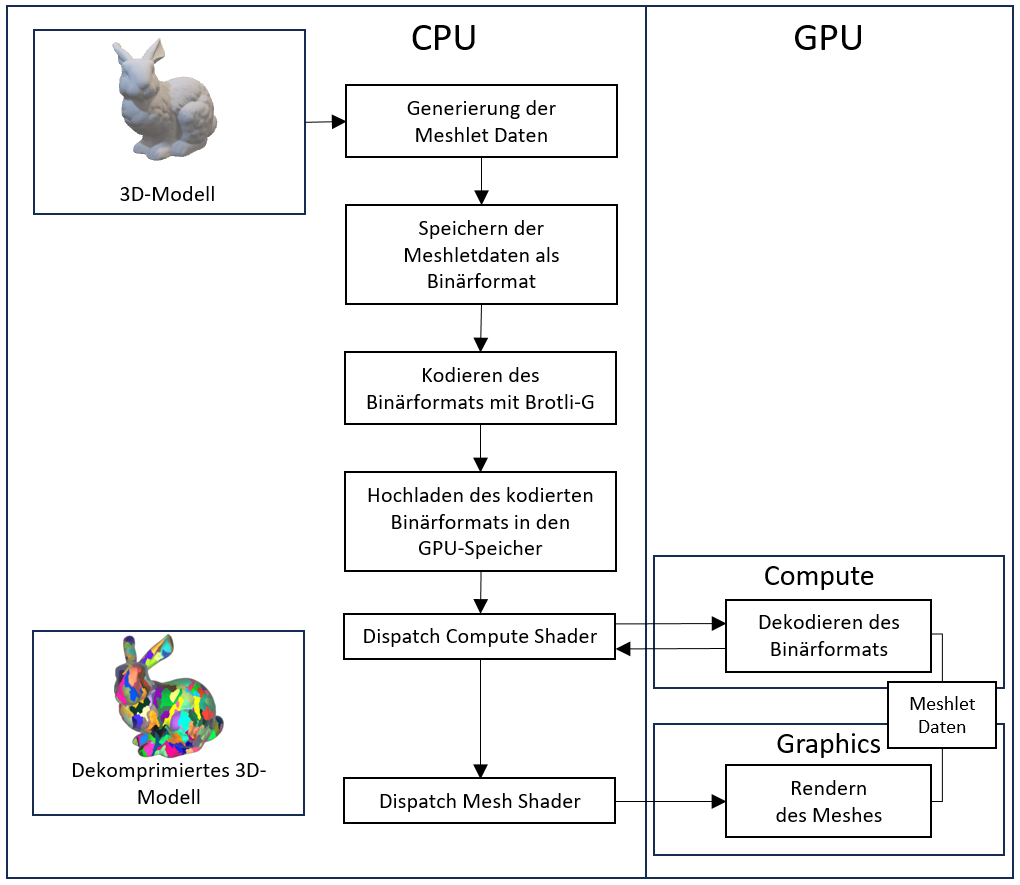
\includegraphics[scale=0.6]{Bilder/Ablauf_Projekt.png}
  \caption[Flussdiagramm Ablauf]{\textbf{Flussdiagramm Ablauf} Abbildung der Dekompressionspipeline.}
  \label{fig:projekt}
\end{figure}

Ist dieser Schritt abgeschlossen, könnten die Daten der UAV auf der CPU ausgelesen werden, die Buffer der Mesh Shader verwendet gefüllt werden und in den GPU RAM geschrieben werden.
Dieser Schritt ist jedoch als unnötig anzusehen, wenn nicht noch zusätzliche Informationen mit dem dekomprimierten Dreiecksnetz berechnet werden müssen.
Der Output Buffer des Brotli-G Dekodierers beinhaltet schon die benötigten Meshlet Daten, um das Dreiecksnetz zu rekonstruieren.
So kann ein GPU Buffer außerhalb von Brotli-G angelegt werden, den Brotli-G als Output Buffer verwendet.
Dadurch wird dieser Buffer nicht freigegeben, nachdem der Dekompressionsschritt von Brotli-G abgeschlossen ist.
Abschließend übergibt man dem Mesh Shader den Output Daten Buffer und kann aus diesem das Dreiecksnetz rekonstruieren.

\subsection{Mesh Shader}
\label{susbsec:mesh_shader}

  \section{Task und Mesh Shader}
Die Architektur, auf der die neuartigen RTX-GPUs von Nvidia aufbauen, erweitert die Möglichkeiten, wie die Parallelisierung von GPUs genutzt werden kann.
Mit der GeForce RTX 20er Serie wurden die ersten GPUs mit der Turing Architektur veröffentlicht, die sich auch an Privatpersonen richtet.
Als großer Verkaufspunkt wurde bereits früh mit den Möglichkeiten von Real-time Raytracing und Deep Learning durch Tensor Core geworben \cite{Burgess2020}. 
Eine wesentliche Änderung an der Grafikpipeline wird jedoch bis heute noch relativ wenig Beachtung geschenkt.
Mit dem Shader Model 6 hat NVidia ihre sogenannte "next-generation shading Pipeline" vorgestellt.
Damit wird eine Alternative zur traditionellen Shading Pipeline gestellt, die dem Entwickler mehr Freiheit überlässt, die Parallelisierbarkeit der GPU zu nutzen.
Der Mesh Shader hat die Eigenschaften des Compute Shaders \ref{subsec:compute_shader}, der Daten auf der GPU parallel verarbeiten kann.
Auch Geometrie Daten können mithilfe des Compute Shaders berechnet werden, jedoch ist der Compute Shader kein Teil der traditionellen Grafikpipeline und findet dadurch seinen Nutzen auch außerhalb des Renderings \cite{Ilett2022}.
Mit der \textit{Mesh Shading Pipeline} wurde die Möglichkeit der Parallelisierung des Compute Shaders mit der neuen Rendering Pipeline verknüpft.
Anders als bei der herkömmlichen Grafikpipeline erhält der Mesh Shader seine Daten direkt vom Speicher. 
Dadurch öffnen sich Türen für den Entwickler, da er komprimierte Daten direkt in den GPU Speicher laden kann, um die Daten dann effizienter auf dieser zu dekomprimieren.


\subsection{Meshlets}
\label{subsec:meshlets}
Um die neuartigen Shader für das Rendering zu verwenden, wird empfohlen, das gesamte Mesh in kleinere Subsets, sogenannte Meshlets, zu unterteilen. 
Die traditionelle Grafikpipeline verarbeitet die Daten des Dreiecksnetzes in serieller Manier. 
Dadurch kommt es jedoch zu Bottlenecks.
In der traditionellen Pipeline werden Vertex und Primitiven zugeschnitten und in kleine Clustern verarbeitet.
Dazu wird der Primitive Distributor vor der Vertex Shader Stage aufgerufen.
Dieser liest die Daten des Index Buffers und generiert dementsprechend möglichst performant diese Cluster an Daten.
Der Schritt des Primitive Distributor ist jedoch eine fixed-function Stage der Grafikpipeline, wodurch der Entwickler keinen direkten Zugriff hat.
Das hat zur Folge, dass die Cluster nicht auf die Bedürfnisse des Entwicklers und dessen Implementierung angepasst werden können.
Zuzüglich werden die Cluster zu jedem Frame, bzw. vor jedem Aufruf der Pipeline neu generiert.
Dieser Schritt ist redundant, sollte das Dreiecksnetz zur Laufzeit unverändert bleiben \cite{Carvalho2022}, \cite{Kubisch2018}. \newline

Durch die Compute Shading Natur des Mesh Shaders ist der Input der Daten nicht mehr festgelegt wie bei der traditionellen Pipeline.
Dadurch kann der Entwickler seine eigenen Implementationen zur Generierung von Meshlets verwenden.
Anders als bei der herkömmlichen Grafikpipeline werden Meshlets auf CPU Ebene erstellt.
Dazu werden Vertex Positionen und Indizes benötigt.
Die Anzahl der Vertices und Primitiven muss im Vorfeld festgelegt werden.
Die Auswahl der Meshletgröße ist abhängig von der verwendeten GPU.
So wird im NVidia Blogpost \glqq Introduction to Turing Mesh Shaders\grqq\ eine maximale Anzahl an Vertices von 64, und Primitiven von 126 empfohlen. 
Es werden 126 statt 128 Primitiven empfohlen, da 4 Byte für die Anzahl der Primitiven verwendet werden, die im selben Block Speicher enthalten sein sollen, bzw. keinen weiteren Block beanspruchen sollen \cite{Kubisch2018}.
Arseny Kapoulkine hat verschiedene Meshletgrößen miteinander verglichen.
Er ist zu dem Schluss gekommen, dass 64 Vertices und 84 Primitives am effizientesten ist, insbesondere dann, wenn im Task Shader Culling an den einzelnen Meshlets betrieben wird.
Des weiteren ist die Empfehlung des Blogposts nach eigenen Tests zwar ein guter Maßstab, jedoch wird im Durchschnitt viel Speicher des Primitiven Buffers ungenutzt bleiben, da die 126 Primitiven mit 64 Vertices nie erreicht werden \cite{Kapoulkine2023}.

\subsection{Implementierung Mesh Shader}
\label{subsec:meshshaderimpl}
Wie im vorherigen Unterkapitel angekündigt muss das Dreiecksnetz auf der CPU zu Meshlets geschnitten werden. 
Dazu wurde in dieser Arbeit er Meshoptimizer von Zeux verwendet \cite{Zeux}. 
[Implementierung von Zeux beschreiben]
Die Funktion \glqq meshopt\_buildMeshlets\grqq\ nimmt als Eingabeparameter die maximale Anzahl an Vertices und Primitiven (Kap.\ref{subsec:meshlets}), die Vertex und Index Daten sowie drei leere Buffer.
Der Buffer \textit{meshlet\_indices} wird die neuen Index Daten enthalten, mit denen die Primitiven berechnet werden können.
Der \textit{meshlet\_vertices} Buffer beinhaltet die einzigartigen Vertices des Dreiecksnetzes (Kap~\ref{subsec:primitive_subgroups}).
Der letzte Buffer wird in dieser Arbeit als \textit{Meshlet Descriptor} bezeichnet.
Der Einfachheit halber wird er im Code jedoch einfach als \textit{meshlets} implementiert.
Der Meshlet Buffer setzt sich auch folgenden Elementen zusammen
\begin{itemize}
\item Vertex Count: Die Anzahl der Vertices V in dem Meshlet mit dem Index i
\item Primitive Count: Die Anzahl der Primitives P in dem Meshlet mit dem Index i
\item Vertex Offset: Die Menge an Schritten im Vertex Buffer, um an die Vertices des i-ten Meshlets zu gelangen
\item Primitive Offset: Die Menge an Schritten im Index Buffer um an die Primitives des i-ten Meshlets zu gelangen
\end{itemize}

Mit den Informationen der originalen Vertexdaten und der drei neu generierten Buffer \textit{meshlet\_indices}, \textit{meshlet\_vertices} und \textit{meshlets}, kann nun der Mesh Shader gefüttert werden.
Zunächst müssen die während des Build-Vorgangs kompilierten Shader gelesen werden.
Diese enthalten Informationen zum Layout der Root Signature, die daraufhin per API-Call erstellt wird.
Bevor die Meshlet Daten an den Mesh Shader übergeben werden können, müssen diese in einen GPU Buffer geschrieben werden, damit diese anschließend in den GPU RAM geschrieben werden können.
Wenn das alles gemacht ist können in der Commandlist der Constant Buffer und die benötigten Meshletdaten über die DirectX12 API-Calls SetGraphicsRootConstantBuffer und SetGraphicsRootShaderRessourceView gesetzt werden.

\subsection{Mesh Shader Implementation}
\label{subsec:mesh_shader_impl}
Im Codeabschnitt~\ref{lst:shadercode} ist ein einfacher Mesh Shader zu sehen.
Im Mesh Shader wird die Root Signature entsprechend den Anforderungen gesetzt.
Minimal wird ein StructuredBuffer für jeden der auf der CPU generierten Meshlet Buffer benötigt.
Um dem Endresultat 3-Dimensional wirken zu lassen, wird ein ConstantBuffer verwendet, der die\textit{model}, \textit{modelView} und \textit{modelViewProjection} Matrix beinhaltet. 
Zusätzlich dazu nimmt der Constant Buffer noch ein boolean, um zu steuern, das die Meshlets farbig hervorgehoben werden.
Zunächst wird das aktuelle Meshlet aus dem \textit{Meshlet Descriptor Buffer} genommen.
Die SV\_GroupID stellt in dieser Implementierung den aktuellen Index der Meshlets dar.
Um den lokalen Index des aktuellen Meshlets zu bekommen, muss die SV\_GroupThreadID verwendet werden.
Die aktuelle GroupID wird in einzelne Threads unterteilt, damit die GPU sich bei der parallelen Verarbeitung nicht in die queere kommt.
Die Anzahl der Threads wird mittles \textit{[NumThreads(128, 1, 1)]} im Mesh Shader, oder, falls vorhanden, im Task Shader festgelegt.

\newpage \begin{lstlisting}[language = C++, caption = Mesh Shader Main, label=lst:shadercode]
[RootSignature(ROOT_SIG)]
[NumThreads(128, 1, 1)]
[OutputTopology("triangle")]
void main(
    in uint gtid : SV_GroupThreadID,
    in uint gid : SV_GroupID,
    out vertices VertexOut verts[64],
    out indices uint3 tris[84]
)
{
  Meshlet m = Meshlets[gid];
  uint3 primitive;

  SetMeshOutputCounts(m.VertCount, m.PrimCount);
  
  if (gtid < m.PrimCount)
  {
    primitive = GetPrimitive(m, gtid);
    tris[gtid] = primitive;
  }
  
  if (gtid < m.VertCount)
  {
    uint vertexIndex = GetVertexIndex(m, primitive[0]);
    verts[gtid] = GetVertex(gid, vertexIndex);
  }
}
\end{lstlisting}

\subsection{Das auf der GPU zu dekodierende Binärformat}
\label{subsec:binary_format}
[Eventuell nicht als eigenes Unterkapitel]

  \section{Kompressionsstandard Brotli-G}
\label{sec:brotlig}
In vielen Anwendungsfällen wird auf Kombinationen von Kompressionsalgorithmen gesetzt.
[QUELLE für Kompression]
Auch Brotli macht sich mehrere Algorithmen zunutze.
Google hat für die Entwicklung von Brotli eine eigene Implementierung des Deflate Algorithmus verwendet.
Das Ergebnis der Kompression besteht aus einer Reihe an Meta Blöcken.
Anstelle der kompletten Daten teilt Brotli den Datensatz in logische Blöcke ein, damit ein besseres Kompressionsergebnis erzielt werden kann.
So wird jeder dieser Blöcke einzeln komprimiert, und zusammen mit den Header Informationen für die gesamten Daten in das Brotli Format geschrieben.
Um die Daten zu komprimieren wird eine Kombination des LZ77 Algorithmus verwendet, um duplizierte Zeichenketten zu erkennen, und einer Huffman-Kodierung um Präfix freie Codewörter zu generieren.
Jeder Meta Block hat dabei seine eigene Huffman-Kodierung.
So sind Überschneidungen von Codewörtern in unterschiedlichen Meta Blöcken möglich, während ein Präfix freier Code in einem Meta Block gewährleistet ist.
Der LZ77 Algorithmus hat zusätzlich noch die Möglichkeit, in einem zuvor kodierten Meta Block nach duplizierten Zeichenketten suchen, sollte diese Zeichenkette noch im Schiebefenster vorhanden sein \cite{rfc7932}. \newline

Um eine parallele Dekompression zu ermöglichen, musste AMD bei Brotli-G einige Veränderungen an den Algorithmen vornehmen.
Zum einen kann die Größe des Schiebefensters abweichen.
Das kommt auf die Größe der Eingabedaten an.
Um die Parallelisierung der Dekompression zu gewährleisten muss auf die Verwendung von vorherigen Meta Blöcken verzichten, und das Schiebefenster zu Beginn eines neuen Meta Blocks zurücksetzen \cite{AMD2024}. \newline

Um die verwendeten Algorithmen besser zu verstehen werden sie in den folgenden Kapiteln genauer betrachtet.

\subsection{LZ77}
\label{subsubsec:lz77}
Der LZ77 (\textit{Lempel-Ziv77}) Algorithmus gehört zu der Gruppe der Phrasenkodierung und ist ein verlustfreier, auf einem Wörterbuch basierender Algorithmus.
Der Algorithmus komprimiert sequentielle Zeichenketten.
Dabei kann dieser auf jeder Art von Daten, egal wie der Inhalt und die Größe aussieht, angewendet werden.
Ob es sich lohnt, diesen anzuwenden, ist jedoch von den Daten abhängig.
Beispielsweise sind Bilder ein schlechter Anwendungsfall, da sich die Informationen nur im Ausnahmefall wiederholen, und es deutlich bessere Kompressionsalgorithmen zur Komprimierung dieser gibt.
Das Ziel des LZ77 Algorithmus ist lediglich, redundante Informationen zusammenzufassen. \newline

Bevor der Algorithmus beschrieben wird, werden die benötigten Elemente definiert:

\begin{enumerate}
\item{Eingabestrom:} Die zu kodierenden Daten
\item{Symbol:} Ein willkürlich gewähltes Element des Eingabestroms
\item{Datenfenster:} Alle Symbole vom Start des Eingabestroms bis zum aktuell betrachteten Symbol
\item{Vorschaufenster:} Ein Buffer fester Größe der Symbole vom aktuell betrachteten Symbol bis zum Ende des Buffers enthält
\item{Schiebefenster:} Daten- und Vorschaufenster
\item{Codewort:} Ein Codewort bestehend aus dem Offset, der Lauflänge und des zu kodierenden Symbols
\end{enumerate}

Der Ablauf des Algorithmus besteht aus folgenden Schritten:

Zu Beginn des Algorithmus wird das Datenfenster auf den Start des Eingabestroms gesetzt.
Dieses Fenster ist zunächst leer.
Das Vorschaufenster wird vom Start des Eingabestroms mit Symbolen gefüllt, bis dieses voll ist.
Zunächst wird das erste Symbol kodiert.
Dafür verwendet der LZ77 Algorithmus ein Tupel in der Form von (\textit{Position}, \textit{Lauflänge}) und abschließend das zu kodierende Symbol.
Dem Wörterbuch noch nicht bekannt Symbole werden neue Symbole mit (0, 0)Symbol hinzugefügt.
Nach jedem Schritt wird das Schiebefenster um die Lauflänge der kodierten Symbole im Eingabestrom verschoben
\cite{lz2023}.

\subsubsection{Kodierung eines Codewortes}
\label{subsubsec:kodierung_codewort}
Zur Veranschaulichung wird das Codewort \glqq laufenraufen\grqq\ mit dem LZ77 Algorithmus kodiert und anschließend wieder dekodiert.
Daten- und Vorschaufenster haben in diesem Beispiel eine Kapazität von jeweils sechs Symbolen. \newpage
\begin{table}[H]
\centering
\begin{tabular}{|l|l|l|l|}
\hline
\textbf{Datenfenster} & \textbf{Vorschaufenster} & \textbf{restliches Codewort} & \textbf{Kodierung} \\ \hline
                      & laufen                   & raufen                       & (0, 0)l            \\ \hline
l                     & aufenr                   & aufen                        & (0, 0)a            \\ \hline
la                    & ufenra                   & ufen                         & (0, 0)u            \\ \hline
lau                   & fenrau                   & fen                          & (0, 0)f            \\ \hline
lauf                  & enrauf                   & en                           & (0, 0)e            \\ \hline
laufe                 & nraufe                   & n                            & (0, 0)n            \\ \hline
laufen                & raufen                   &                              & (0, 0)r            \\ \hline
aufenr                & aufen                    &                              & (6, 4)n            \\ \hline
\end{tabular}
\label{tab:lz77_encode_table}
\caption{LZ77 Kodierungs Beispiel}
\end{table}

Eine Besonderheit die zunächst nicht intuitiv ist, ist die Konstruktion des letzten Codewortes in diesem Beispiel.
Die Symbolsequenz \glqq aufen\grqq\ mit der Kodierung \textit{(6, 4)n} könnte auch mit einem Offset von fünf kodiert werden.
Im Normalfall würde die Symbolsequenz auch so kodiert werden.
Da jedoch das Symbol \glqq n\grqq\ das letzte Symbol des zu kodierenden Worts ist, und es so kein weiteres, zu kodierendes Symbol gibt, muss die Länge um eins reduziert werden, und das letzte Symbol kodiert werden. \newline

Aus dem Beispiel geht hervor, das die Auswahl der Buffergröße gut gewählt werden muss, damit der Algorithmus effektiv verwendet werden kann.
Wäre in dem Beispiel das Datenfenster lediglich Platz für vier statt fünf Symbole, hätte die Symbolsequenz \glqq aufe\grqq nicht als ganzes kodiert werden können.
Die weiteren Iterationen der Lempel-Ziv Algorithmen haben statt einem lokalen Wörterbuch (Datenfenster) ein globales Wörterbuch verwendet.
Durch die große Anzahl an Vergleichen erreicht der LZ77 Algorithmus ein besseres Kompressionsverhältnis als der LZ78 Algorithmus, benötigt für die Kompression jedoch länger.
Wie lange das Komprimieren der Daten dauert ist jedoch nicht wichtig für diese Arbeit.
Der interessante Punkt ist die Dekompressionsgeschwindigkeit.
Der LZ77 Algorithmus ist bedeutend schneller bei der Dekomprimierung als bei der Komprimierung \cite{Choudhary2015}. \newpage

\subsubsection{Dekodierung eines Codeworts}
\label{subsubsec:dekodierung_codewort}
In diesem Abschnitt soll aus der Kodierung das zuvor festgelegte Codewort dekodiert werden.
Als Ergebnis aus der Kodierung erhalten wir den Ausgabestrom: \newline
 \textit{(0, 0)l}, \textit{(0, 0)a}, \textit{(0, 0)u}, \textit{(0, 0)f}, \textit{(0, 0)e}, \textit{(0, 0)n}, \textit{(0, 0)r}, \textit{(6, 4)n}. \newline
Jetzt gilt es, das Datenfenster zu füllen.
In einem Schritt der Dekodierung wird das Datenfenster überprüft, sollte Offset und Lauflänge ungleich 0 sein.
Falls vorhanden werden die Daten des Datenfensters mit dem Symbol der aktuell zu dekodierenden Symbol dem Codewort hinzugefügt.
Im nächsten Schritt wird die Symbolsequenz an die Symbole des Datenfensters verkettet, bis dieses voll ist.
Anhand des letzten Schrittes der Dekompression sieht man wie der Algorithmus eine duplizierte Zeichenkette erkennt.
In diesem Beispiel wird die Zeichenkette \textit{aufe} mit einem Offset von 6 und einer Lauflänge von 4 aus dem Datenfenster gelesen, und mit dem Symbol \textit{n} verkettet.
Die Dekodierung ist nach diesem Schritt abgeschlossen.
\newline
\begin{table}[H]
\centering
\begin{tabular}{|l|l|l|}
\hline
\textbf{Kodierung} & \textbf{Datenfenster}         & \textbf{Codewort} \\ \hline
(0, 0)l            &                               & l                 \\ \hline
(0, 0)a            & l                             & la                \\ \hline
(0, 0)u            & la                            & lau               \\ \hline
(0, 0)f            & lau                           & lauf              \\ \hline
(0, 0)e            & lauf                          & laufe             \\ \hline
(0, 0)n            & laufe                         & laufen            \\ \hline
(0, 0)r            & laufen                        & laufenr           \\ \hline
{\color[HTML]{009901}(6, 4)n}            & {\color[HTML]{009901} aufe}nr & laufenr{\color[HTML]{009901} aufen}      \\ \hline
\textbackslash 0   & raufen 					   & laufenraufen 		\\ \hline
\end{tabular}
\label{tab:lz77_decode_table}
\caption{Dekodierung mit dem LZ77-Algorithmus}
\end{table}

Wie zu sehen ist, ist der LZ77 Algorithmus sowohl leicht verständlich als auch effektiv, wodurch er seinen Nutzen in vielen Anwendungen findet.
Seine Weiterentwicklungen nennen sich LZ78 und LZW, die zwar dem LZ77 Algorithmus technisch überlegen sind, aufgrund von Patenten jedoch nicht so eine große Rolle spielen wie die erste Iteration von Lempel und Ziv.
In Kombination mit anderen Techniken wie der Huffman Codierung bildet der LZ77-Algorithmus jedoch die Grundlage vieler leistungsstarker Kompressionsstandards, die heute in vielen Applikationen zu finden sind [QUELLE!!!]. \newline


\subsection{Huffman-Kodierung}
\label{subsec:huffman}
Eine gewisse Ähnlichkeit zu dem in der Einleitung angerissenen Thema des Morse Codes enthält die von Brotli verwendete Huffman-Kodierung.
Die Huffman-Kodierung ist eine Methode zur verlustfreien Datenkompression und gehört zur Art der Codewort basierten Entropiekodierung.
Ähnlich wie beim Morse Code, werden Symbole durch Bitfolgen substituiert.
Was beim Morse Code als langes und kurzes Signal galt, ist im Huffman Code eine 0 oder 1.
Mit der Huffman-Kodierung werden häufig auftretende Symbole durch kurze Bitfolgen dargestellt.
Dementsprechend erhalten Symbole mit geringer Auftrittswahrscheinlichkeit ein langes Codewort.
Bei der Betrachtung des Morse Codes fällt auf, dass nicht jeder Buchstabe die selbe Anzahl an Signalen beansprucht.
Die Codewörter im Morse Code haben sich nämlich ebenfalls die Eigenschaft der Auftrittswahrscheinlichkeiten zunutze gemacht.
Die im englischen Alphabet meist verwendeten Codewörter \glqq E\grqq\ und \glqq T\grqq\ werden beide mit jeweils einem Signal dargestellt.
Das \glqq E\grqq\ wird mit einem kurzen, während das \glqq T\grqq\ vom langen Signal dargestellt wird.
Mithilfe dieser Eigenschaft verbrauchen Symbole, die häufig auftreten, weniger Platz im Bitstrom \cite{Moffat2019}.
Histogramm ....

\subsubsection{Konstruktion einer Huffman-Kodierung}
\label{subsubsec:konstruktion_huffman}
Zur Konstruktion eines Huffman Codes wird ein Binärbaum generiert.
Die zu kodierenden Symbole werden als Blätter des Baumes betrachtet.
Der Baum wird sozusagen von \glqq unten nach oben\grqq\ bzw. von \glqq Blätter nach Wurzel\grqq aufgebaut. \newline
In jedem Schritt werden die zwei Symbole oder Knoten mit der geringsten Auftrittswahrscheinlichkeit zu einem neuen Knoten verbunden.
Die Auftrittswahrscheinlichkeit des neu erstellten Knotens ist die Summe der Auftrittswahrscheinlichkeiten der verbundene Symbole/Knoten.
Sobald die Wurzel des Baumes erreicht ist, also die Auftrittswahrscheinlichkeit bei 1 liegt, ist die Huffman-Kodierung abgeschlossen.
Jedem Zweig des Baums wird zusätzlich eine 0 oder 1 zugewiesen.
Ob der linke Kindknoten die 0 und der rechte Kindknoten die 1 bekommt, oder anders herum ist nicht wichtig, und kann von Implementierung zu Implementierung abweichen.
Wichtig ist nur zu beachten, das dies im gesamten Baum konsistent durchgezogen wird.
Die Codewörter für jedes Symbol sind abzulesen, indem die Beschriftungen der Zweige als ein Bitstrom interpretiert werden, beginnend von der Wurzel.

Um den Vorteil dieser Eigenschaft zu Veranschaulichen, kann ein Vergleich mit dem \textit{fixed length Code (FLC)} hilfreich sein.
Anders als \textit{Variable Length Code (VLC)} Verfahren wie die Huffman-Kodierung, wird jedem Symbol eines FLCs ein Codewort fester Länge zugewiesen.
Die Auftrittswahrscheinlichkeit spielt bei der Erstellung von Codewörtern also keine Rolle.
Um einen Vergleich zu ziehen kann die mittlere Codewortlänge des Alphabets, mit folgenden Symbolen betrachtet werden.

\begin{table}[h]
\centering
\begin{tabular}{ccccc}
\toprule
\textbf{\textit{\(S_i\)}} & {A} & {B} & {C} & {D} \\
\midrule
\textbf{\textit{\(P_i\)}} & 0.6 & 0.2 & 0.1 & 0.1\\
\bottomrule
\end{tabular}
\end{table}

Die Formel zur Berechnung der mittleren Codewortlänge des FLCs lautet
\begin{equation*}
\bar{l} = \lceil \log_2(N) \rceil
\end{equation*}
Wird das aus 4 Symbolen bestehende Beispielalphabet mittels FLC kodiert, ist die Codewortlänge \(l_i\) eines jeden Symbols = 2, wodurch auch die mittlere Codewortlänge bei 2,0 \textit{Bits/Symbol} liegt.

Die Konstruktion des Binärbaums, aus dem die Codewörter entnommen werden können ist in Abb.~\ref{fig:huffman_example} zu sehen.

\begin{figure}[htb]
  \centering  
  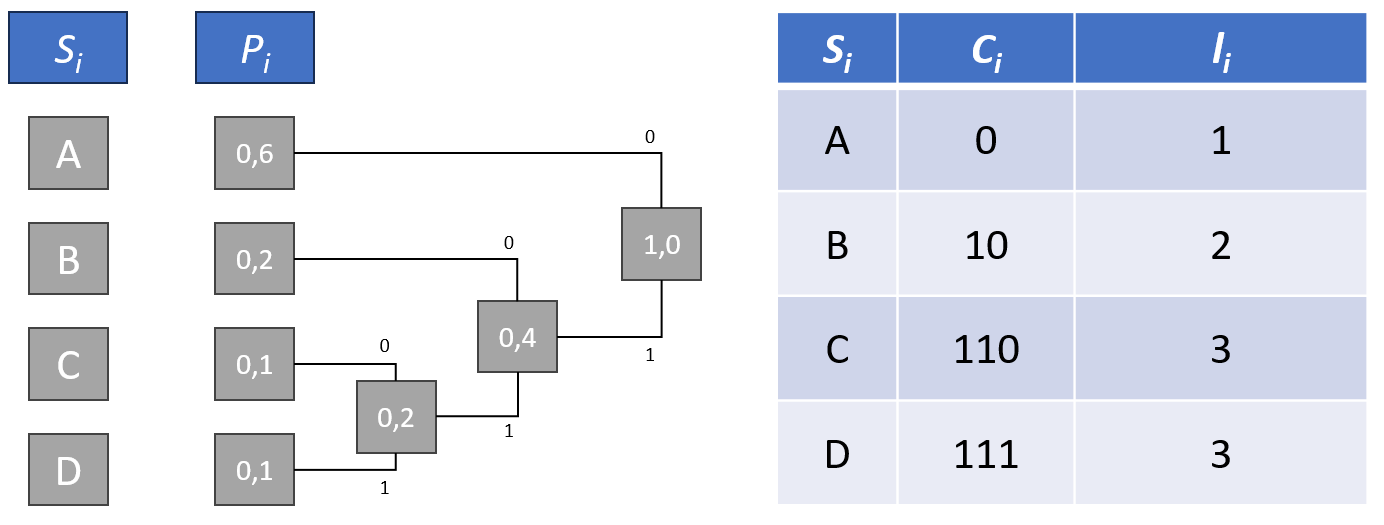
\includegraphics[scale=0.4]{Bilder/Huffmancode_beispiel.png}
  \caption[Huffman Code Beispiel]{\textbf{Erstellen eines Huffman Codes} Die Abbildung zeigt die Konstruktion eines Binärbaums und der daraus resultierenden Codewörter für die Symbole}
  \label{fig:huffman_example}
\end{figure}

\subsubsection{Resultate einer Huffman-Kodierung}
\label{subsec:huffman_res}
Aus diesem Beispiel kann der Nutzen der Huffman-Kodierung anhand von Werten ausgedrückt werden. \newline
Um die mittlere Codewortlänge einer Huffman-Kodierung zu berechnen, wird die Formel
\begin{equation*}
\bar{l} = \sum_{i=1}^{n} p_i \cdot l_i
\end{equation*}
benötigt \newline

Aus dem Beispiel ergibt sich eine mittlere Codewortlänge von 1,6 \textit{Bits/Symbol} bei einer Huffman-Kodierung.
Im Vergleich zu einem FLC werden also 0,4 \textit{Bits/Symbol} gespart. 
Die Formel für das Kompressionsverhältnis lautet:
\begin{equation*}
C_r = \frac{\text{Eingabegröße}}{\text{Ausgabegröße}}
\end{equation*}

Da sich bei einer Huffman-Kodierung lediglich die Codewortlängen ändern, kann der FLC als Eingabe-, und der Huffman Code als Ausgabegröße in der Formel verwendet werden.
So ergibt sich ein Kompressionsverhältnis von:
\begin{equation*}
C_r = \frac{\lceil \log_2(N) \rceil}{\sum_{i=1}^{n} p_i \cdot l_i}
\end{equation*}
% TODO: Problem mit Zeilenumbruch deshalb gerade zwei equations
\begin{equation*}
C_r = \frac{2,0 \ \text{Bits/Symbol}}{1,6 \ \text{Bits/Symbol}} = 1,25
\end{equation*}

Die Effektivität der Huffman-Kodierung hängt stark von der Verteilung der Symbole in der Datenquelle ab. 
Wenn der konstruierte Binärbaum stark balanciert ist, bedeutet dies, dass die Codewörter für die einzelnen Symbole ähnliche Längen haben. 
In solchen Fällen ist die Huffman-Kodierung weniger effektiv, da sie weniger Redundanz in den Daten ausnutzen kann.

Redundanz beschreibt den unnötigen Aufwand zu Repräsentation einer Information.
Die Aufgabe der Huffman-Kodierung ist die Minimierung der \textit{Codierungsredundanz}.


Im Gegensatz dazu profitiert die Huffman-Kodierung enorm von einer ungleichen Verteilung der Symbole, bei der bestimmte Symbole deutlich häufiger auftreten als andere. 
Dadurch können kürzere Codewörter für häufige Symbole und längere Codewörter für seltene Symbole verwendet werden, was zu einer besseren Kompression führt.

Allerdings ist die Huffman-Kodierung anfällig für Veränderungen in der statistischen Verteilung der Symbole. 
Wenn sich die Auftrittswahrscheinlichkeiten im Laufe der Anwendung ändern oder wenn sie falsch berechnet wurden, kann dies zu einer Verschlechterung der Kompression führen. 
Im Extremfall kann es vorkommen, dass das Symbol mit der höchsten Auftrittswahrscheinlichkeit das längste Codewort erhält, was die Effizienz der Codierung erheblich beeinträchtigt. 
Daher ist es wichtig, dass die Statistik der Symbole regelmäßig überprüft und aktualisiert wird.
Um das zu bewerkstelligen kann eine adaptive Huffman-Kodierung verwendet werden. 
Anstelle einer festen Symbolstatistik wird bei der adaptiven Huffman-Kodierung die Statistik nach dem Kodieren eines Symbols überprüft und aktualisiert. 
Adaptive Algorithmen liefern zu Beginn einer Kodierung noch keine guten Ergebnisse, da die Symbolstatistik bei wenigen Symbolen nicht Aussagekräftig ist \cite{Jeon1998}. 

\subsection{GZIP}
\label{subsec:gzip}
Brotli-G misst sich mit anderen Kompressionsstandards wie GZip und Deflate.
Der Deflate Algorithmus beschreibt eine Kombination aus dem LZ77 Algorithmus und der Huffman-Kodierung
[Wahrscheinlich kein eigenes Kapitel. Lieber Deflate Algorithmus in anderen Kapiteln erwähnen]

\subsection{Brotli-G Compute Shader}
\label{subsec:brotlig_compute}
Das komprimierte Dreiecksnetz soll mittels Brotli-G's GPU Dekodierer dekodiert werden.
Da Brotli-G mit der Grafik-API DirectX12 arbeitet, wird eine GPU benötigt die das Shader Model 6 unterstützt.
Für die Verwendung des GPU Dekodierers wird also eine NVidia Grafikkarte mit der Turing-Architektur benötigt \cite{Burgess2020}.
Diese erkennt man am RTX Präfix vor der Modellnummer.
Bei AMD Grafikkarten muss mindestens die RDNA-2 Architektur verbaut sein.
Mit Grafikkarten aus der AMD RX6000er Reihe für RDNA-2, und der RX7000er Reihe für RDNA-3 kann der GPU Dekodierer verwendet werden.
Brotli-G definiert ihren GPU Dekodierer in der Shader-Sprache \textit{high-level shader language (HLSL)} und ist als Compute Shader definiert (Kap.~\ref{subsec:compute_shader}). \newline

Da es sich bei Brotli-G um eine Modifikation des Brotli Formats handelt, wurde der Bitstrom des Kodierers angepasst.


\subsection{CPU Ebene}
\label{subsec:brotlig_cpu}
Queries Buffers etc

  \section{Ergebnisse}
\label{sec:ergebnisse}
Dieses Kapitel widmet sich den Ergebnissen dieser Arbeit. 
Im Kap.~\ref{subsec:ablauf} wurde eine grobe Schilderung gegeben, wie die Pipeline aussieht, die ein beliebiges 3D-Modell durchläuft, bis es gezeichnet wird.
Im ersten Anlauf wurde ein Datensatz bestehend aus 11 unterschiedlichen 3D-Modellen durch diese Pipeline geschickt. 
Dabei wurde der Kompressionsstandard Brotli-G untersucht. 
Wichtige Gesichtspunkte für die Auswertung sind das Kompressionsverhältnis, und die Geschwindigkeit, in der die komprimierten Dreiecksnetze dekomprimiert werden. 
Die visuelle Qualität muss im ersten Anlauf zwangsweise unverändert bleiben, da Brotli-G verlustfrei komprimiert (Kap.~\ref{subsec:brotli}). 
Die Ergebnisse des ersten Ablaufs sind in der nachfolgenden Abb.(einfügen) dokumentiert.

\begin{figure}[htb]
  \centering  
  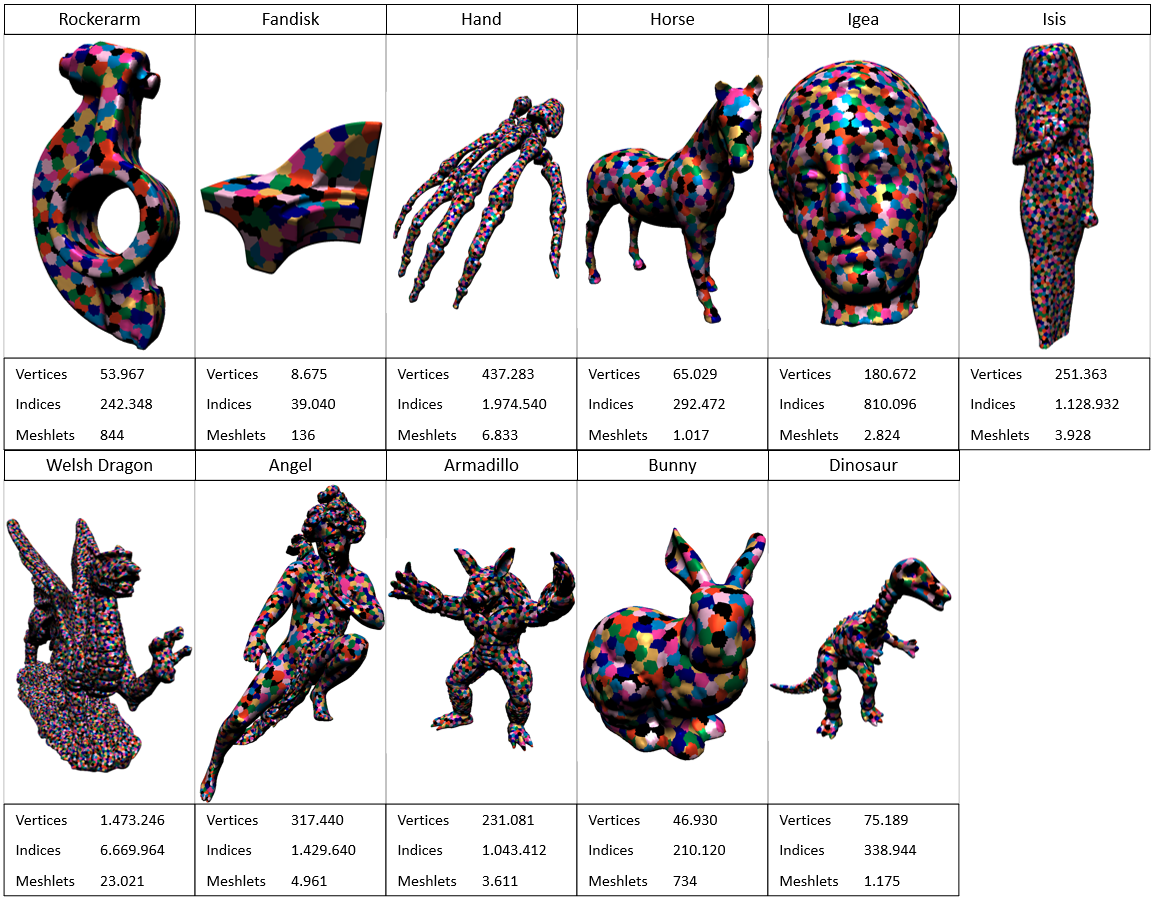
\includegraphics[scale=0.5]{Bilder/Ergebnisse_zusammen.png}
  \caption[Der verwendete Datensatz]{\textbf{Der verwendete Datensatz} Die Abbildung zeigt alle Dreiecksnetze mit der Anzahl an Geometrie und Topologie. }
  \label{fig:mesh_shading_pipeline}
\end{figure}

Der Datensatz besteht aus vielen unterschiedlichen 3D-Modellen unterschiedlicher Größe. 
Von einem sehr kleinen Modell der \textit{Fandisk}, mit 136 Meshlets, bis hin zu einem \textit{Welsh Dragon}, der aus 23.021 Meshlets besteht, werden nun die Ergebnisse des Brotli-G Kodierers ausgewertet und analysiert.

\subsection{Die Ergebnisse des Datensatzes}
\label{subsec:auswertung1}
Betrachten wir zunächst das Dreiecksnetz mit der geringsten Anzahl an Vertices/Indizes/Meshlets. 
Die Ergebnisse des Kodierers sind sehr vielversprechend. 
Die 366.536 Bytes des Originalmodells komprimiert Brotli-G auf 160.200 Bytes und erreicht somit ein Kompressionsverhältnis von 2,29.
Auffällig sind hierbei jedoch die Dekompressionszeiten für dieses sehr kleine Modell. 
Bei der Größe des Modells und der doch sehr hohen Dekompressionszeit für den GPU-Dekodierer wird eine Bandbreite von 0,054 GiB/s erreicht, was deutlich weniger ist, als was der PCIe-Bus der GPU zulässt, die für den Versuch verwendet wurde.

\begin{figure}[htb]
  \centering  
  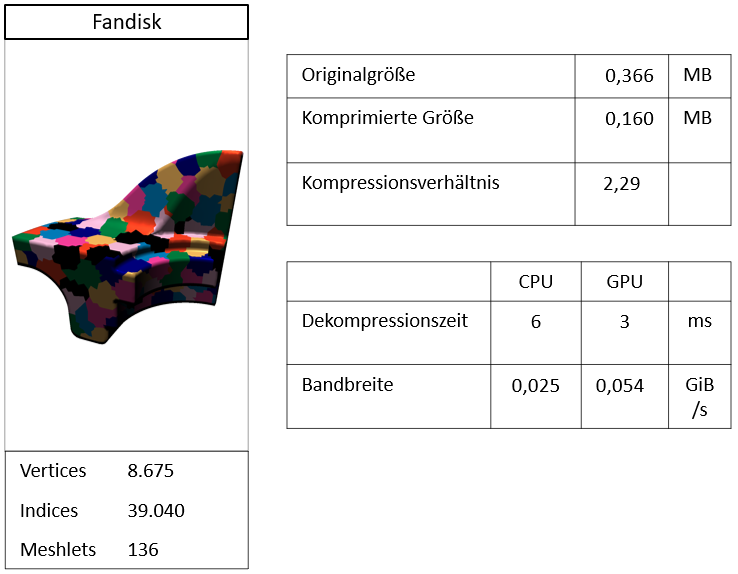
\includegraphics[scale=0.75]{Bilder/ergebnisse/fandisk.png}
  \caption[Fandisk Kompressionsergebnis]{\textbf{Fandisk Kompressionsergebnis} Das kleinste Dreiecksnetz aus dem Datensatz, und seine Ergebnisse}
  \label{fig:mesh_shading_pipeline}
\end{figure}

Um die niedrige Bandbreite zu analysieren, können die Ergebnisse des Welsh Dragons betrachtet werden. 
Dieser besteht aus sehr viel mehr Geometrie und Topologie, was sich in der Größe des Modells widerspiegelt. 
Der Welsh Dragon hat eine Originalgröße von 62.406.096 Bytes, die auf 31.716.764 Bytes komprimiert wurde. 
Das entspricht einem Kompressionsverhältnis von 1,97.
Viel interessanter hierbei sind jedoch die Dekompressionszeit und die daraus resultierende Bandbreite. 
Der GPU Brotli-G GPU-Dekodierer benötigt nicht unbedingt viel mehr Zeit für den Welsh Dragon (7 ms) gegenüber der Fandisk (3 ms).
Bei Anbetracht der komprimierten Größe der beiden Dreiecksnetze fällt auf, das der Welsh Dragon sehr viel mehr Daten benötigt. 
Während die Dekompression des Welsh Dragons etwas mehr als das Zweifache an Zeit verglichen mit der Fandisk benötigt, ist die komprimierte Größe des Welsh Dragons etwa 200x so groß wie diese.
Das Ergebnis davon ist in der Bandbreite zu sehen, die beim Welsh Dragon sehr viel besser ist, jedoch noch immer sehr weit von den gewünschten Werten entfernt ist.
Die parallele Dekodierung des Brotli-G Dekodierers scheint daher erst bei größeren Datensätzen richtig effektiv zu werden.

\begin{figure}[htb]
  \centering  
  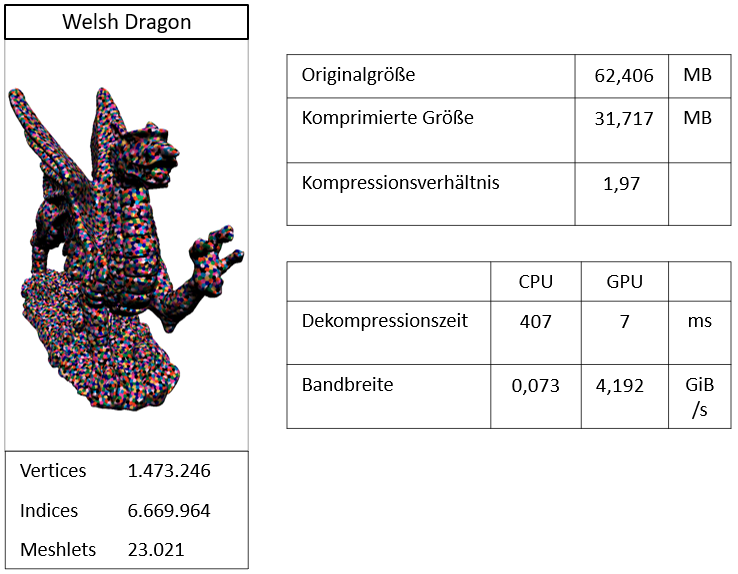
\includegraphics[scale=0.75]{Bilder/ergebnisse/welshdragon.png}
  \caption[Welsh Dragon Kompressionsergebnis]{\textbf{Welsh Dragon Kompressionsergebnis} Das größte Dreiecksnetz aus dem Datensatz, und seine Ergebnisse}
  \label{fig:mesh_shading_pipeline}
\end{figure}

\subsection{Auswertung der quantisierten Vertex-Daten}
\label{subsec:auswertung2}
Im zweiten Anlauf werden die Vertex Daten vor der Komprimierung zu 16-Bit floating point values quantisiert.
Ziel davon ist, die Bits mit geringer Wertigkeit, die nur wenig zur Struktur des 3D-Modells beitragen, loszuwerden.
Die hinteren 16 Bit einer 32 Bit Gleitkommazahl beansprucht genau soviel Speicher wie die vorderen 16 Bit.
Während die vorderen Bits jedoch die grobe Position des Vertex, oder auch die Richtung der Normalen, sind die Bits mit geringerer Wertigkeit für sehr feine Details wichtig.
Für ein visuell ansprechendes Dreieck sind 16 Bit pro Komponente ausreichend, außer in Bereichen, in denen diese feine Granularität sehr wichtig ist, wie z.B. bei medizinischen Anwendungen. \newline

Um die Qualität zu visualisieren, sieht man in Abb.~\ref{fig:bunny} das Stanford Bunny einmal mit 16, und einmal mit 32 Bit Vertex Attributen.

\begin{figure}[htb]
  \centering  
  \includegraphics[scale=0.45]{Bilder/bunny_quantisiert.png}
  \caption[Quantisiertes Stanford Bunny]{\textbf{Quantisiertes Stanford Bunny} Die Abbildung zeigt eine Gegenüberstellung des Bunny mit 32 Bit Vertex Attributen und dem Bunny mit den quantisierten 16 Bit Vertex Attributen }
  \label{fig:bunny}
\end{figure}

Bei der Gegenüberstellung sind die Unterschiede kaum erkennbar, was sehr hilfreich ist, wenn die Kompression mit Brotli-G betrachtet wird.
Um einen Vergleich der Ergebnisse zu ziehen, wird wieder der Welsh Dragon zur Auswertung der Kompressionsergebnisse verwendet.
Lediglich die Quantisierung der Vertex Daten spart rund \textit{29 \%} der Größe vor der Komprimierung.
Die Originalgröße von 44.727.144 Bytes wird anschließend von Brotli-G auf 17.260.728 Bytes komprimiert, was einem Kompressionsverhältnis von 2,59 entspricht.
Die Dekomprimierung auf der GPU nimmt mit 6 ms in etwa so viel Zeit in Anspruch wie der Welsh Dragon mit 32 Bit Gleitkommazahlen.
Dadurch ergibt sich eine Bandbreite von \textit{2,706 \ GiB/s}. \newline

Im Anhang sind die Ergebnisse für alle Dreiecksnetze aus dem Datensatz ersichtlich.
Dabei fällt auf, das der Welsh Dragon bei der Betrachtung der Kompressionsverhältnisse kein Einzelfall ist.
Betrachtet man die Ergebnisse von quantisierten und nicht quantisierten Dreiecksnetzen, ist klar zu erkennen, das die quantisierten Dreiecksnetze nicht nur weniger Speicherplatz beanspruchen.
Das Kompressionsverhältnis ist im Durchschnitt des Datensatzes bei den quantisierten Dreiecksnetzen um \textit{18,82 \%}.

\begin{figure}[htb]
  \centering  
  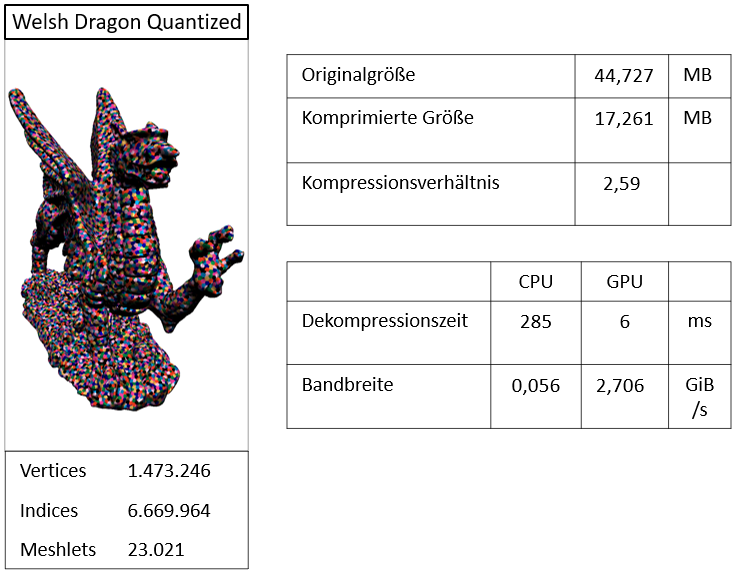
\includegraphics[scale=0.75]{Bilder/ergebnisse/welshdragon_q.png}
  \caption[Welsh Dragon Kompressionsergebnis quantisiert]{\textbf{Welsh Dragon Kompressionsergebnis quantisiert} Die Ergebnisse des quantisierten Welsh Dragon }
  \label{fig:quantized_welsh_dragon}
\end{figure}

\subsection{Die Resultate von Michelangelos David}
\label{subsec:auswertung3}
Wie in den anderen Versuchen erkannt wurde, wird eine bestmögliche Bandbreite bei großen Dreiecksnetzen erreicht.
Dafür wird in diesem Abschnitt ein Teil eines großen Dreiecksnetzes des Davids ausgewertet.
Leider legt Brotli-G eine maximale GPU Buffer Größe von 1 GB fest, wodurch ein maximal zu dekodierender Block eingeschränkt wird.
Sollte ein größeres Dreiecksnetz dekodiert werden, muss dieses sinngemäß zugeschnitten werden.
Die Haare des David bestehen aus fünf kleinen Teilstücken, die zusammengetragen eine Größe von rund 760 MB aufweisen, und so einen Großteil der maximalen Buffergröße verwenden.
Die kleinen Teilstücke wurden auf der CPU nacheinander eingelesen, und in ein gemeinsames Binärobjekt geschrieben, das von Brotli-G kodiert worden ist. \newline
Brotli-G hat die Größe des Davids von 759.567.128 Bytes auf 326.929.888 Bytes komprimiert, und somit ein Kompressionsverhältnis von 2,32 erreicht.
Auf der GPU wurde dieses in 65 ms dekomprimiert, wodurch eine Bandbreite von $\mathit{4,682 \ GiB/s}$ erreicht wurde.

\begin{figure}[htb]
  \centering  
  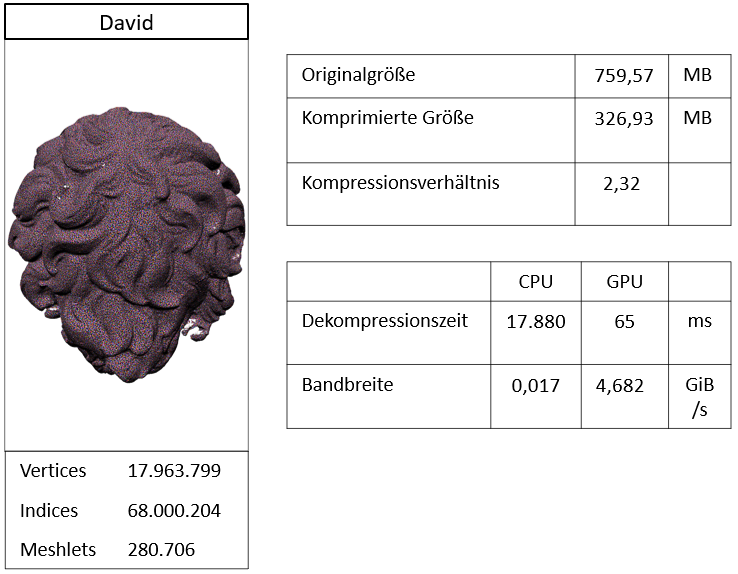
\includegraphics[scale=0.75]{Bilder/ergebnisse/david.png}
  \caption[David Kompressionsergebnis]{\textbf{David Kompressionsergebnis} Ein Teil von dem großen Dreiecksnetz des Davids }
  \label{fig:david_ergebnis}
\end{figure}

Auch bei diesem Dreiecksnetz wird zusätzlich noch ein Ergebnis mit quantisierten Vertex Attributen durchgeführt.
Die Quantisierung reduziert die Originalgröße des Davids um etwa 200 MB.
Nachdem das quantisierte Dreiecksnetz von Brotli-G komprimiert wurde, sind von den 544.001.528 Bytes noch 115.287.560 Bytes übrig.
Daraus ergibt sich das beste Kompressionsverhältnis in dieser Arbeit mit 4,72.
Dafür ist die Bandbreite wiederum etwas schlechter gegenüber dem David mit 32 Bit Gleitkommazahlen für die Vertex-Attribute.
Aus einer Dekompressionszeit von 37 ms und der Größe von 115,29 MB ergibt sich dafür eine Bandbreite von $\mathit{2,983 \ GiB/s}$. \newline

Anhand der Ergebnisse scheint der Scan des Davids von Michelangelos sehr detailliert zu sein.
Das bedeutet, dass die kleinen Details des Davids von der Quantisierung entfernt wurden, sodass Brotli-G die Daten schöner komprimieren konnte.
Hier besteht eine sehr große Differenz der Kompressionsverhältnisse von Originalwerk und dem quantisierten Dreiecksnetz.
Während das originale Dreiecksnetz schon ein gutes Kompressionsverhältnis von 2,32 aufweist, ist das Ergebnis des quantisierten Dreiecksnetzes mit 4,72 überragend.

\begin{figure}[htb]
  \centering  
  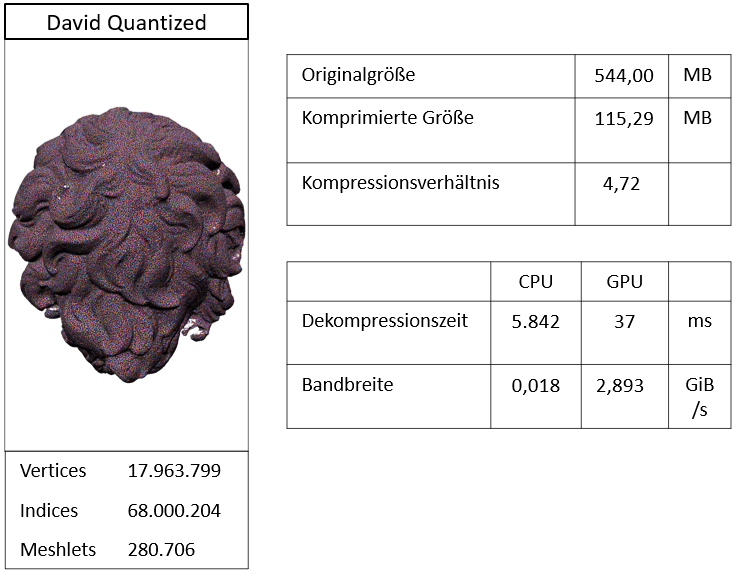
\includegraphics[scale=0.75]{Bilder/ergebnisse/david_q.png}
  \caption[David Kompressionsergebnis quantisiert]{\textbf{David Kompressionsergebnis quantisiert} Ein Teil von dem großen Dreiecksnetz des Davids mit quantisierten Vertex Attributen }
  \label{fig:david_ergebnis}
\end{figure}

  \section{Fazit}
\label{sec:fazit}
Auf den ersten Blick scheint die Bandbreite mit der Größe der komprimierten Daten zu korrelieren.
Wie in den Ergebnissen zu sehen, bietet die Quantisierung dazu noch eine nicht zu verachtende Reduktion der Speichergröße.
Die Kombination aus Quantisierung und der anschließenden Kompression mit Brotli-G scheint dazu noch bessere Kompressionsverhältnisse zu liefern. \newline
Die Ergebnisse aus Kap.~\ref{sec:ergebnisse} sollen zuletzt bewertet und analysiert werden.
Die Bewertungsmaße liegen bei den Kompressionsverhältnissen und der Bandbreite.

\subsection{Analyse der Dekompressionszeit und Bandbreite}
\label{subsec:ana_bandwidth}
Eine Möglichkeit für die geringe Bandbreite scheint auf den ersten Blick die Größe der komprimierten Daten zu sein.
Auffällig ist nämlich die geringe Bandbreite bei kleinen Dreiecksnetzen wie der Fandisk.
Mit einer komprimierten Größe von 0,160 MB benötigt diese am wenigsten Speicherplatz, und erreicht eine Bandbreite von \textit{0,054 GiB/s}.
Weitere Beispiele sind das Bunny mit einer Größe von \textit{1,067 MB} und einer Bandbreite von \textit{0,503 GiB/s}, der Dinosaur mit 1,713 MB und einer Bandbreite von 0,825 GiB/s und der Rockerarm mit 1,139 MB und einer Bandbreite von \textit{0,399 GiB/s}.
Es scheint dabei zudem eine untere Grenze der Dekompressionszeit zu geben.
Diese liegt bei den sehr kleinen Dreiecksnetzen bei \textit{2 ms - 3 ms}.
Bei Betrachtung der mittelgroßen Dreiecksnetze des Datensatzes scheint die Dekompressionszeit jedoch nicht wie erwartet zuzunehmen.
Die Dekompressionszeit der Igea, des Armadillo und des Angels beträgt ebenfalls jeweils \textit{3 ms}.
Die Größe der komprimierten Dreiecksnetze liegt bei \textit{4,033 MB, 4,486 MB und 7,239 MB}.
So sind diese ca. 3 - 4 mal so groß wie die kleinen Dreiecksnetze. 
Bei einer höheren Dateigröße und gleichbleibender Dekompressionszeit steigt natürlich die Bandbreite. 
Die Bandbreite der Igea liegt bei \textit{1,473 GiB/s}, des Armadillos bei \textit{1,415 GiB/s} und der des Angels bei \textit{2,346 GiB/s}.
Die Ergebnisse sind zwar besser, aber dennoch noch nicht auf einem hohen Niveau. \newline

Eine mögliche Erklärung für diese untere Schranke kann die Zeitrechnung des Brotli-G Dekodierers sein.
Die Zeitrechnung des Brotli-G Dekodierers misst nicht ausschließlich die Dauer des Compute Shaders.
Der Umstand einer unteren Schranke bei 2 ms kann am Overhead der API-Aufrufe von DirectX12 liegen.
Die Zeitrechnung beginnt demnach bei dem Aufruf der decodeGPU Methode und endet, nachdem der Destruktor der Klasse das Objekt zerstört, das den Compute Shader mit Daten gefüttert und ausgeführt hat. \newline

Die Ergebnisse der zwei größten Dreiecksnetze des Datensatzes scheinen die These zu stützen, dass die kleinen Dreiecksnetze nicht effektiv von Brotli-G verarbeitet werden oder ein zu großer prozentualer Anteil an Overhead das Ergebnis verfälscht.
Die Hand erreicht eine Bandbreite von \textit{2,218 GiB/s} bei einer komprimierten Größe von \textit{8,195 MB}.
Bezüglich der Bandbreite erreicht der Welsh Dragon \textit{4,192 GiB/s}, mit einer komprimierten Größe von \textit{31,717 MB}.
Auch hier scheint die Korrelation von komprimierter Größe und Bandbreite weiterzubestehen.

\subsection{Analyse der Kompressionsverhältnisse}
\label{subsec:ana_ratios}
Die Kompressionsverhältnisse, die nur mittels Brotli-G erzielt wurden, sind gut.
Bei dem Datensatz ergibt sich ein durchschnittliches Kompressionsverhältnis von \textit{1,99} über alle Dreiecksnetze verteilt.
Das größte Kompressionsverhältnis verzeichnet die Fandisk mit \textit{2,29}, während das Horse das geringste Kompressionsverhältnis von \textit{1,84} besitzt.
Bei den Kompressionsverhältnissen gibt es keine Überraschungen oder Auffälligkeiten wie bei der Bandbreite.

\subsection{Analyse der quantisierten Dreiecksnetze}
\label{subsec:ana_quantized}
Der Großteil der Daten eines Dreiecksnetzes besteht aus seiner Geometrie \cite{Jakob2017}.
Bei Betrachtung der Komponenten ist zwar erkennbar, das es wesentlich mehr Dreiecke, und somit auch mehr Indizes, als Vertices gibt.
Wenn als Topologie eine \textit{Triangle List} verwendet wird, gelangt man auf ein Verhältnis von 
\begin{equation*}
V:T = 1:2
\end{equation*}
Da ein Dreieck aus 3 Indizes besteht, enthält ein Dreiecksnetz von dieser Topologie in etwa 6 Indizes pro Vertex (Euler's Formel) \cite{Engstad2011}.
Angenommen, ein Vertex bestehe lediglich aus Positionen und Normalen, wie es bei dem verwendeten Datensatz dieser Arbeit der Fall ist.
So enthält ein Vertex ohne Kompression der Daten
\begin{equation*}
3 * 4 \ \text{Byte} = 12 \ \text{Byte}
\end{equation*}
Gleitkommazahlen für die Position im 3-dimensionalen Raum.
Und nochmal so viele Byte für die Normalen.
Da gib dem Vertex eine Größe aus 24 Byte.
Ein unkomprimierter Index wird in einem Integer ohne Vorzeichen gespeichert, der 4 Byte beansprucht \cite{Microsoft2021a}. \newline
Beachtet man das Verhältnis der Euler Formel bei Dreiecksnetzen, enthalten 6 Indizes mit 192 Bit die gleiche Datenmenge wie ein Vertex mit Position und Normale.
Zu beachten ist jedoch, dass neben der Position auch Texturkoordinaten, Farben, Tangenten und Bitangenten in den Vertex Attributen vorhanden sein können. \newline
Jedenfalls ist erkennbar, dass die Vertices einen maßgeblichen Einfluss auf die Datengröße nehmen.
Bei jedem einzelnen Dreiecksnetz des Datensatzes ist eine Reduktion der Daten von \textit{28,4 \%} zu sehen.
Die Quantisierung mindert jedoch nicht nur die originalen Eingabedaten.
Vergleicht man die von Brotli-G komprimierten Originaldaten und die von Brotli-G komprimierten Daten seines quantisierten Gegenübers, so ist eine Reduktion der komprimierten Daten von durchschnittlich \textit{39,71 \%} möglich.
Die meisten Dreiecksnetze sind in einem Bereich von \textit{38 \% - 42 \%}.
Die Ausreißer liegen jedoch nicht weit entfernt von diesem Bereich, mit dem Armadillo der mit \textit{32,6 \%} am schlechtesten abgeschnitten hat, während der Welsh Dragon mit \textit{45,6 \%} die größte Reduktion der Originaldaten hat.
Diese Diskrepanz der Prozente ist gut erkennbar, wenn die Kompressionsverhältnisse von quantisierten und nicht quantisierten Dreiecksnetzen betrachtet werden.
Hier wird schnell klar, das der Armadillo mit \textit{6,42 \%} den geringsten Zuwachs der Kompressionsverhältnisse erlangt hat, während der Welsh Dragon mit \textit{32,5 \%} den besten Zuwachs der Kompressionsverhältnisse verzeichnet.
Diese komprimierten Daten können direkt aus einem Speichermedium in den GPU-RAM hochgeladen werden, wo sie vom Brotli-G Compute Shader dekomprimiert und vom Mesh Shader gerendert werden. \newline

Das verbesserte Kompressionsverhältnis stammt von dem losgewordenen Rauschen der Originaldaten.
Die Daten des Dreiecksnetzes werden für gewöhnlich in einer Genauigkeit repräsentiert, die für die Darstellung einfacher 3D-Modelle nicht benötigt wird.
Wenn diese richtig quantisiert werden, ist der Verlust an visueller Qualität meist so gering, das diese kaum auffällt.
Die Fließkommazahl ist somit frei von Signalrauschen, das sehr schwer zu kodieren ist, da diese Zeichenfolgen oft zufällig oder willkürlich sind.
\begin{figure}[htb]
  \centering  
  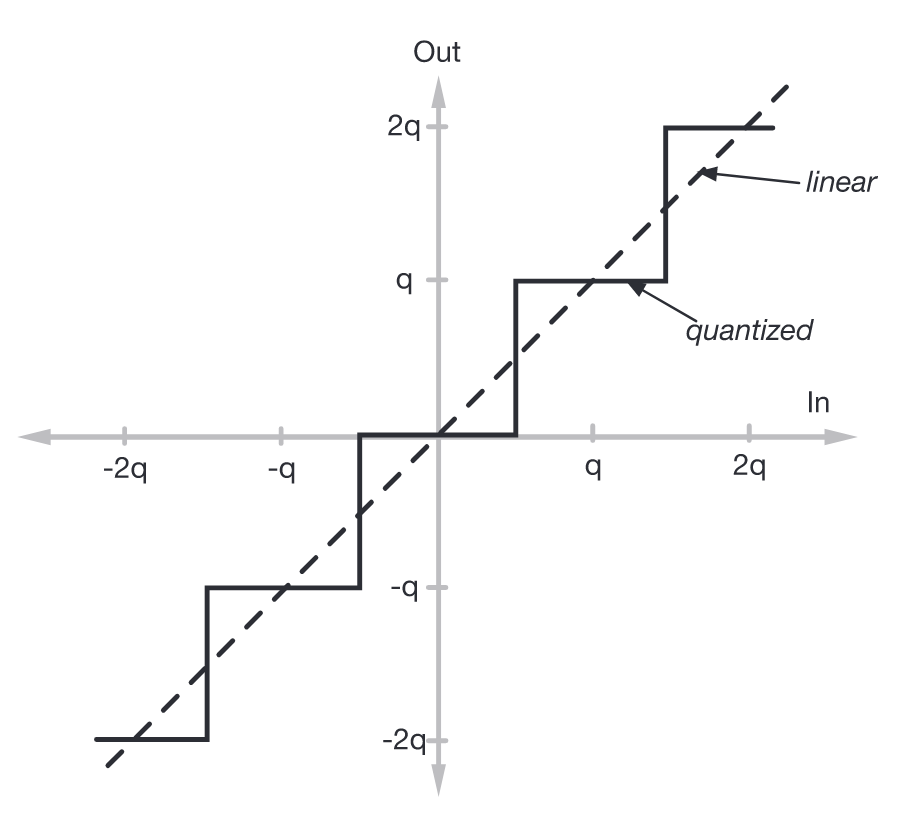
\includegraphics[scale=0.35]{Bilder/quantization.png}
  \caption[Mid-Tread Quantisierer]{\textbf{Mid-Tread Quantisierer} Die Abbildung zeigt eine Gegenüberstellung von den möglichen Werten vor der Quantisierung (gestrichelte Linie) und den möglichen Werten nach der Quantisierung (durchgezogene Linie.
  Die Abbildung stammt aus \cite{Bennett2020} }
  \label{fig:mid-tread_quantizer}
\end{figure}

\subsection{Ausblick für spätere Arbeiten}
\label{subsec:ausblick}
Wie zu sehen ist, ergeben sich durch die Komprimierung mittels Brotli-G gute Kompressionsverhältnisse.
Die Auswertung der Ergebnisse zeigt auch, dass weitere Verfahren zur Datenkompression nicht nur zu einer direkten Datenreduktion führen, sondern auch die Ergebnisse von Brotli-G verbessern können.
In dieser Arbeit wurde der Einsatz von der Quantisierung verwendet.
Weitere Verfahren, die in Kombination mit Brotli-G getestet werden können, sind die \textit{prädiktive Kodierung}, \textit{Triangle Traversal Encoding} oder \textit{Connectivity Compression} \cite{Jakob2017}.
Da sich die Indizes lediglich in einem bestimmten kleinen Intervall bei der Verwendung von Meshlets befinden, würde sich zusätzlich anbieten, diese nicht einzeln in einer 4 Byte Datenstruktur wie einem Integer zu speichern, sondern jeweils drei Indizes (bei einer Triangle List eine Primitive) in einen Integer zu packen. \newline

Nach einem Blogpost auf GPUOpen von AMD wurde die Version 1.1 von Brotli-G mit dem Compressonator Version 4.5 veröffentlicht.
Die Tests die in dem Blogpost behandelt werden, richten sich zwar an Texturen, die Ergebnisse von der neuen Version von Brotli-G sind dennoch sehenswert.
Im Vergleich zur alten Version reduziert der Compressonator mit der neuen Brotli-G Version die komprimierten Texturen im Durchschnitt um weitere \textit{10 \% - 15 \%}, in besonders guten Fällen sogar um \textit{20 \%} \cite{Levesque2024}.
Die Brotli-G Version 1.1 wurde leider erst gegen Ende dieser Arbeit veröffentlicht, wodurch die vorliegenden Ergebnisse auf der Version 1.0 bestehen.
Die besseren Ergebnisse des Compressonators lassen auf zukünftig bessere Resultate und vor allem auf eine effektivere Ausnutzung der Bandbreite des PCIe-Busses hoffen.
Die Ergebnisse dieser Arbeit in der Hinsicht der Dekompressionszeit und Bandbreitenausnutzung sind selbst bei den größeren Dreiecksnetzen weit von gewünschten Werten entfernt.
Für die Versuche wurde die Grafikkarte \textit{Radeon RX 6650 XT} von AMD verwendet.
Diese soll laut Datenbankeintrag eine maximale Bandbreite von \textit{280 GB/s}, also zum Vergleich umgerechnet ungefähr \textit{260 GiB/s} erreichen.
Es ist zwar unwahrscheinlich, an dieses Maximum zu gelangen, dennoch wäre eine bessere Ausnutzung der Bandbreite wünschenswert. \newpage
\begin{figure}[htb]
  \centering  
  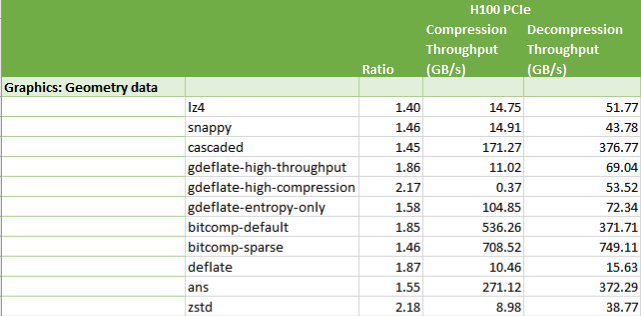
\includegraphics[scale=0.70]{Bilder/nvComp_geometry_results.png}
  \caption[NVIDIAs nvCOMP Testergebnisse]{\textbf{NVIDIAs nvCOMP Testergebnisse} In der Abbildung sind die Ergebnisse der NVIDIA Bibliothek nvCOMP zu sehen, die verlustfreie Datenkompression und Dekompression unter Verwendung einer GPU ausführt.
  Die Abbildung ist von NVIDIAs öffentlicher Developer Website. https://developer.nvidia.com/nvcomp }
  \label{fig:nvCOMP}
\end{figure}
In der Abbildung.~\ref{fig:nvCOMP} ist zu sehen. welche Kompressionsverhältnisse unterschiedliche Algorithmen der nvCOMP Bibliothek.
Neben dieser sind die Bandbreiten der Kompression und Dekompression.
Das Ziel ist es nicht, die Bandbreiten dieser Arbeit mit den Ergebnissen von nvCOMP zu vergleichen.
Dabei spielt auch nicht nur der verwendete Datensatz eine Rolle.
Die verwendete GPU aus Abbildung~\ref{fig:nvCOMP} ist nicht für Privatpersonen gebaut worden.
Vor allem ist die \textit{Tensor Core GPU} H100 für Unternehmen gedacht, die GPUs für aufwendige Rechenarbeiten benötigen.
Dementsprechend erzielt diese sehr viel bessere Ergebnisse, als die für Privatpersonen geeignete RX 6650 XT.
Dennoch kann aus dieser Abbildung entnommen werden, das eine sehr viel höhere Bandbreite erzielt werden kann, als es in dieser Arbeit der Fall war.



\finishHSCdocument